\documentclass[a4paper,11pt]{book}
%=============================  Font selection  ==============================
\usepackage[T1]{fontenc}
    % Defines the encoding of the characters output by LaTeX.  With T1,
    % characters are encoded with 8 bits, allowing many accented European
    % characters to be encoded with a single glyph.  This makes hyphenation
    % of words containing these characters possible.  Otherwise, by default,
    % TeX uses 7 bits per character and cannot hyphenate accented words.
    % T1 is also called "Cork Encoding":
    %    https://en.wikipedia.org/wiki/Cork_encoding
    % It's kind of old though: it's LaTeX that's lagging behind.
    % XeTeX and LuaTex are UTF-8 all the way.
    
%=======================  UTF-8 support in the source  =======================
\usepackage[utf8]{inputenc}
    % Allows me to input accented characters directly from my keyboard instead
    % of having to type G\"odel.
    % Note that bibtex does not support that, so in my .bib files I must still
    % enter the annoying characters.

\usepackage{lmodern}

%===============================  DEPENDENCIES  ==============================
\RequirePackage{snapshot}
    % Generates a .dep files that contains all the files (pictures and stuff)
    % on which a document depends.

%==================================  FLOATS  =================================

% According to
% http://tex.stackexchange.com/questions/96350/problem-with-algorithmic-and-hyperref
% if I want to have hyperref working with algorithm, I must
% first load float, then hyperref, then algorithm.
% Putting float here solves the TOC links to the algorithms, otherwise they'd
% all point to page 1.
% Also, putting float-algo-hyper creates a massive amount of warnings for pretty much
% every algo command like \State.
\usepackage{float}

\usepackage{placeins}
    % Brings \FloatBarrier command. It forces Tex to typeset all remaining floats
    % at that point and doesn't include a \clearpage afterwards.
    % Nice to flush all the floats before beginning a new section.

\usepackage[font=footnotesize,labelfont=bf,margin=1cm]{caption}
    % So that I can add long captions under figures.
    
    % It provides me with \caption* that does not appear in the list of
    % figures but formats the text like \caption does.  It also lets me
    % use line breaks in the caption, and even bullet/enumerated lists.
    
    % The margin of 1 cm makes it easier to see what's caption and what's
    % main-body text when there's a float on top of a page.

\usepackage{subcaption}
    % Lets me have labels such as a) b) c) inside a figure environment.
    % Unfortunately something is broken, I cannot give labels to these
    % subcaptions when hyperef is active, the pdf compiler hangs forever.
    % Seems to be a common problem.

\usepackage{rotating}
    % Used to display long tables in landscape mode.

%http://tex.stackexchange.com/questions/38972/how-to-forbid-latex-to-put-text-between-figures
\renewcommand\topfraction{0.70}
\renewcommand\bottomfraction{0.70}
\renewcommand\textfraction{0.20}
%http://www-rohan.sdsu.edu/~aty/bibliog/latex/floats.html
% Alter some LaTeX defaults for better treatment of figures:
    % See p.105 of "TeX Unbound" for suggested values.
    % See pp. 199-200 of Lamport's "LaTeX" book for details.
    %   General parameters, for ALL pages:
%    \renewcommand{\topfraction}{0.9}	% max fraction of floats at top
%    \renewcommand{\bottomfraction}{0.8}	% max fraction of floats at bottom
    %   Parameters for TEXT pages (not float pages):
\setcounter{totalnumber}{4} % default 3    % 2 may work better
\setcounter{topnumber}{4} % default 2
\setcounter{bottomnumber}{4} % default 1
%    \setcounter{dbltopnumber}{2}    % for 2-column pages
%    \renewcommand{\dbltopfraction}{0.9}	% fit big float above 2-col. text
%    \renewcommand{\textfraction}{0.07}	% allow minimal text w. figs
    %   Parameters for FLOAT pages (not text pages):
%    \renewcommand{\floatpagefraction}{0.7}	% require fuller float pages
	% N.B.: floatpagefraction MUST be less than topfraction !!
%    \renewcommand{\dblfloatpagefraction}{0.7}	% require fuller float pages

	% remember to use [htp] or [htpb] for placement

%===============================  BACKMATTER  ================================

\usepackage{makeidx}
    % Needed to build the index.

\usepackage[toc,page]{appendix}
    % Brings \begin{appendices}.
    % toc option creates an "appendices" entry in the table of content.
    % page option creates a page before the first appendix chapter.

%\usepackage[sorting=nyt,citestyle=authoryear,backref=false,]{biblatex}
\usepackage[backend=bibtex,style=authoryear,sorting=nyt]{biblatex}
    % Fantastic bibliography manager that I'll use just for its
    % \citetitle command.
    % For sorting orders, see
    % https://www.sharelatex.com/blog/2013/07/31/getting-started-with-biblatex.html
    % backref does not work with hyperref.
\DefineBibliographyStrings{english}{%
    backrefpage  = {see p.}, % for single page number
    backrefpages = {see pp.} % for multiple page numbers
}
\newcommand{\citeformula}[1]{\text{\citetitle{#1}}}

%===========================  HEADERS AND FOOTERS  ===========================
\usepackage{fancyhdr}
\pagestyle{fancy}
\let\originalchaptermark\chaptermark

\makeatletter
    \renewcommand{\chaptermark}[1]{%
        \if@mainmatter
            \originalchaptermark{#1}%
        \else
            \markboth{#1}{}%
        \fi
    }
\makeatother

% Note: Even pages (E) are on the left, odd (O) pages on the right.
\addtolength{\headheight}{\baselineskip}
\fancyhf{}  % First, start with a clean slate.
\fancyhead[LE,RO]{\thepage}
\fancyhead[RE]{\slshape\nouppercase\leftmark}
\fancyhead[LO]{\slshape\nouppercase\rightmark}
%\renewcommand{\headrulewidth}{\iffloatpage{0pt}{0.4pt}}


\fancypagestyle{plain}{%
    \fancyhf{}
    \fancyfoot[LE,RO]{\thepage}
    \renewcommand{\headrulewidth}{0pt}
    \renewcommand{\footrulewidth}{0pt}
}

\makeatletter
    \def\cleardoublepage{
        \clearpage\if@twoside \ifodd\c@page\else
        \hbox{}
        \vspace*{\fill}
        %\begin{center}
        %This page intentionally contains only this sentence.
        %\end{center}
        \vspace{\fill}
        \thispagestyle{empty}
        \newpage
        \if@twocolumn\hbox{}\newpage\fi\fi\fi
    }
\makeatother


%=================================  TESTING  =================================
\usepackage{lipsum}


%==============================  SUBDIRECTORIES  =============================

\usepackage{import}
    % Facilitates the organization of the book.  I can place each chapter in its own
    % directory, along with its images.
    % Brings /subimport{directory}{tex_file_name_without_extension}.

%===================================  COLOR  =================================

\usepackage[table]{xcolor}
    % The 'table' parameter loads another package that lets me set
    % alternating colors for the rows of a table.
    % xcolor also imports color, which is useful for importing figures saved as
    % PDF+TEX files generated by inkscape.
    
    % Must be loaded before todonotes: todonotes loads color without the [table]
    % option.

%=================================  DRAFTING  ================================

\ifDraft
    \usepackage{todonotes}
        % Big post-its, handy while writing.
\else
    \usepackage[disable]{todonotes}
\fi

%===============================  MATHEMATICS  ===============================

%---------------------------------  FORMULAS  --------------------------------
\usepackage{amsmath}
    % Brings the align environment for lining up equations on the =.

\usepackage{nicefrac}

\usepackage{bm}
    % For bold mathematics.
    % An advantage of using \bm over \mathbf is that \bm keeps the
    % letters slanted in maths.  I use bold letters for vectors,
    % I see no reason to have them typeset upright.
    % Another advantage is that it works on greek letters too.

\usepackage{amssymb}
    % For the Real/Complex/etc. number set symbols via \mathbb.

\usepackage[makeroom]{cancel}
    % For striking out bits of equations that simplify.

\usepackage{stmaryrd}
    % For the llbracket and rrbracket to denote integer intervals.

% Fix the spacing introduced by \left and \right in formulas.
\let\originalleft\left
\let\originalright\right
\renewcommand{\left}{\mathopen{}\mathclose\bgroup\originalleft}
\renewcommand{\right}{\aftergroup\egroup\originalright}

% Macro to wrap something between top corners, useful for Gödel number
% or litteral predicates.
\newbox\gnBoxA
\newdimen\gnCornerHgt
\setbox\gnBoxA=\hbox{$\ulcorner$}
\global\gnCornerHgt=\ht\gnBoxA
\newdimen\gnArgHgt
\def\cornered #1{%
\setbox\gnBoxA=\hbox{$#1$}%
\gnArgHgt=\ht\gnBoxA%
\ifnum     \gnArgHgt<\gnCornerHgt \gnArgHgt=0pt%
\else \advance \gnArgHgt by -\gnCornerHgt%
\fi \raise\gnArgHgt\hbox{$\ulcorner$} \box\gnBoxA %
\raise\gnArgHgt\hbox{$\urcorner$}}
% Use \cornered{blah}.

% Class theory.
\newcommand{\classname}[1]{\mathcal{#1}}
\newcommand{\tuple}[1]{\begin{bmatrix}#1\end{bmatrix}}
\newcommand{\smalltuple}[1]{\big[ \begin{smallmatrix}#1\end{smallmatrix} \big]}

% Category theory.
\newcommand{\catname}[1]{\mathbf{#1}}            % Category name.
\newcommand{\morph}[3]{#1 : #2 \to #3}           % Morphism.
\DeclareMathOperator{\classHom}{hom}             % Class of morphisms.
\DeclareMathOperator{\classOb}{ob}               % Class of objects.
\DeclareMathOperator{\id}{id}                    % Identity morphism.
\DeclareMathOperator{\dom}{dom}                  % Domain.
\DeclareMathOperator{\cod}{cod}                  % Codomain.
\DeclareMathOperator{\apply}{\$}                 % Arrow application. 


% Set theory.
\newcommand{\innerprod}[2]{\langle #1, #2 \rangle}
\newcommand{\innerprodd}[1]{\innerprod{#1}{#1}}
\newcommand{\Innerprod}[2]{\left\langle #1, #2 \right\rangle}
\newcommand{\Innerprodd}[1]{\Innerprod{#1}{#1}}
%\newcommand{\inprod}[2]{\langle #1, #2 \rangle}  % Inner product of two vectors.
%\newcommand{\vangle}[2]{\left(#1, #2\right)}     % Angle between vectors.
\DeclareMathOperator{\spanset}{Sp}               % Span, in the linear algebra sense.
\DeclareMathOperator{\Over}{over}                % (V, *) over F is a vector field.
\DeclareMathOperator{\End}{End}                  % End(X) = set of endomorphisms of X.
\DeclareMathOperator{\Aut}{Aut}                  % Aut(X) = set of automorphisms of X.
\newcommand{\card}[1]{\left\lvert #1 \right\rvert}         % Cardinal of a set.
%
% This command writes a function in the form
%
%    f : A --> B
%        a |-> b
%
% The parameters are f, A, B, a and b in that order:
% f is the function name, A the domain, B the codomain, a an element of A and b an
% element of B.
\newcommand{\func}[5]{
    \begin{array}{rccc}
        #1: & #2 & \to     & #3\\
            & #4 & \mapsto & #5
    \end{array}
}
% For set or list comprehension.
% example: $\{ \comp{(x,y)}{x^2+y^2=1} \}$ renders as {(x,y) | x^2+y^2=1}.
\newcommand{\comp}[2]{#1 \mid #2}


% Scalars.
\newcommand{\abs}[1]{\left\lvert #1 \right\rvert}          % Absolute value of a scalar.
\newcommand{\cp}[1]{\hat{#1}}                    % Complex object.
    % Used as indices:
\newcommand{\re}{r} % Real part.
\newcommand{\im}{i} % Imaginary part.

% Vectors.
\newcommand{\norm}[1]{\left\| #1 \right\|}       % Norm of a vector.
\newcommand{\vect}[1]{\bm{#1}}                   % Real vector.
\newcommand{\vectcp}[1]{\cp{\vect{#1}}}          % Complex vector.
\newcommand{\vectu}[1]{\dot{\vect{#1}}}          % Unit (real) vectors.

% Matrices.
\newcommand{\matr}[1]{\mathrm{#1}}               % Real matrix.
\newcommand{\matrcp}[1]{\cp{\matr{#1}}}          % Complex matrix.
\newcommand{\transp}{^\top}                      % Tranposed of a matrix.

% Trigonometry.
\DeclareMathOperator{\atantwo}{arctan2}            % Arctan(y, x).

% Calculus.
\newcommand{\dif}{\operatorname{d}}              % For integrals: dx dy dz.
\newcommand{\timeavg}[1]{\langle #1 \rangle}
\newcommand{\Timeavg}[1]{\left\langle #1 \right\rangle}

% Bullshit.
\newcommand{\equaldef}{\stackrel{\text{\tiny def}}{=}}

% Probabilities.
\DeclareMathOperator{\prob}{P}

%----------------------------------  LOGIC  ----------------------------------
\usepackage{bussproofs}
\renewcommand{\iff}{\mathbin{\longleftrightarrow}} % More correct than \iff and \implies for
\renewcommand{\implies}{\mathbin{\longrightarrow}} % first-order logic.
\newcommand{\lxor}{\oplus}                         % Logical exclusive or.
\newcommand{\dn}{\mathord{\downarrow}}
\newcommand{\up}{\mathord{\uparrow}}
\newcommand{\entails}{{\enspace}\mathbin{\vdash}{\enspace}}

% Predicates.
\newcommand{\litpred}[1]{\cornered{#1}}
\DeclareMathOperator{\Category}{Category}
\DeclareMathOperator{\Class}{Class}
\DeclareMathOperator{\Monoid}{Monoid}
\DeclareMathOperator{\Evt}{Evt}
\DeclareMathOperator{\Indep}{Indep}
\DeclareMathOperator{\Excl}{Excl}

%---------------------------------  THEOREMS  --------------------------------
\usepackage{amsthm}
\newtheorem{axiom}{Axiom}
\newtheorem{theorem}{Theorem}

%================================  QUANTITIES  ===============================

\usepackage{siunitx}
    % Otherwise I can't write the mu symbol for micrometers.
    % It also brings me the \degree symbol, woo!
    % No decibel though, I need to make this one myself.
    
    % My version of siunitx is too old so I cannot use \DeclareSIUnit to create
    % new units.
\newcommand{\decibel}{dB}  % \DeclareSIunit doesn't work with my version.
\newcommand{\parsec}{pc}
\newcommand{\astronomicalunit}{au}  % Was ua until 2014.
\newcommand{\mass}{M}
\newcommand{\charge}{Q}
\newcommand{\distance}{L}
\newcommand{\duration}{T}
\newcommand{\bit}{bit}

%=================================  PHYSICS  =================================

% Used as indices:
\newcommand{\I}{I} % Incident.
\newcommand{\R}{R} % Reflected.
\newcommand{\T}{T} % Transmitted/refracted.
\newcommand{\power}[1]{\mathcal{#1}}

%================================  CHEMISTRY  ================================

\usepackage[version=3]{mhchem}
    % For chemical formulas.
    % Brings \ce.

\newcommand{\Jlevel}[2]{$J=#1\!\rightarrow\!#2$}
\newcommand{\transition}[3]{\ce{#1}~\Jlevel{#2}{#3}}

%================================  DIAGRAMS  =================================

\usepackage[all]{xy}
\usepackage{tikz}
\usepackage{pgfkeys}

%==================================  LISTS  ==================================

\usepackage{enumitem}
    % Allows customization of bullet-lists and numbered-lists.
    % In particular, allows removing the insane amount of vertical space that latex
    % injects in these lists by default.
    % Usage: \begin{itemize}[noitemsep,nolistsep]
    % noitemsep removes the spacing between the items.
    % nolistsep removes the spacing between the paragraph and the list.
    % Global usage: \setlist[itemize]{noitemsep}
    % Except that this global usage doesn't work on my old installation.


%=================================  PICTURES  ================================

\usepackage{graphicx}
    % Can't have pictures/photos/figures from files without that.
    % Note that vanilla latex will only accept eps while tex2pdf accepts
    % anything except eps.  Go figure...



%=================================  TABLES  ==================================

\usepackage{booktabs}
    % For professional-looking tables.
    % Brings the \toprule, \midrule and \bottomrule.
    % Remember not to use vertical rules in tables: they look cheap.

\usepackage{multirow}
    % How isn't that even standard?

\usepackage{tabularx}
    % Brings the X column type, auto expand to fill the page.

\usepackage{array}
    % Brings >{} and <{} column modifiers to wrap the content into stuff.

% And this is convenient too because it allows me to set the width of a column,
% like p does, but with left/right/center justification.
\newcolumntype{L}[1]{>{\raggedright\arraybackslash}p{#1}}
\newcolumntype{C}[1]{>{\centering\arraybackslash}p{#1}}
\newcolumntype{R}[1]{>{\raggedleft\arraybackslash}p{#1}}

%=============================  CROSS REFERENCES  ============================

% As a rule of thumb, hyperref goes last.  Only a few packages go after.
% cleveref is a well known one.  bookmark is another one.

% According to
% http://tex.stackexchange.com/questions/53191/impact-of-hyperref-when-varioref-and-cleveref-are-used/53193#53193
% one must first load varioref, then hyperref, then cleveref.
% Failure to do so results in lots of hyperrefs warnings and links that do not point to the right place.
\usepackage{varioref}
    % For fancier references that also tell the page number.

\ifPrint
    \usepackage[draft]{hyperref}
\else
    \usepackage[plainpages=false, hypertexnames=false]{hyperref}
    % Requires direct pdf output, therefore all figures should be pdf too.
    % This creates hyperlinks all over the place to jump to figures, references,
    % chapters and all.
    % hypertexnames=false makes the package dumber, allowing it to work even if
    % there are several chapter 1 in the document.
    \hypersetup{
        colorlinks,
        linkcolor={red!50!black},
        citecolor={green!40!black},
        urlcolor={blue!80!black}
    }
\fi
    
%\usepackage[capitalize,noabbrev]{cleveref}
\usepackage[capitalize]{cleveref}
    % Should make the typesetting of cross references more consistent.
    % Note that I needed to install a recent version of this package, the one I had
    % was too old to handle algorithms properly.
    % NOTE that cleveref is confused by the subcaption package.  Whenever you place
    % a label in a subfigure, cleveref hangs forever.  The label at the figure level
    % works fine though.  So, no labeling of subfigures :(.
    %
    % Interesting options:
    %    noabbrev
    %    capitalize
\crefname{appsec}{appendix}{appendices}
\Crefname{appsec}{Appendix}{Appendices}
\crefname{axithm}{axiom}{axioms}
\Crefname{axithm}{Axiom}{Axioms}
\crefname{thmthm}{theorem}{theorems}
\Crefname{thmthm}{Theorem}{Theorems}

%=============================  ALGOS AND CODE  ==============================

% According to
% http://tex.stackexchange.com/questions/113719/cleveref-fails-to-reference-algorithms
% Algorithm must be loaded before hyperref.  Well, it is not true.
\usepackage[chapter]{algorithm}
    % To float algorithms.
\usepackage{algpseudocode}
    % For pseudocode.
\usepackage{listings}
    % For real code.

%===============================  SPECIAL TEXT  ==============================

\hyphenation{aniso-tro-pic iso-tro-pic impe-dance va-cuum algo-rithm algo-rithms col-linear pe-rio-dic tera-hertz}
\newcommand{\radex}{\textsc{radex}}
\newcommand{\Radex}{\textsc{Radex}}

%===========================  WIDOWS AND ORPHANS  ============================

% I hate having a paragraph that has only one line on a page.
% It's made even worse when there's a float cutting the paragraph in two.
% Here, I am telling LaTeX that windows and orphans are infinitely bad.
% http://tex.stackexchange.com/questions/4152/how-do-i-prevent-widow-orphan-lines
\widowpenalty10000
\clubpenalty10000

%===============================  WEIRD THINGS  ==============================

% This thing helps filtering some warnings during debugging.  There often are
% warnings caused by very small overfull hboxes and they `pollute' the log,
% drowning the more critical warnings.  Although I believe that a document
% should compile with zero warning, it also makes sense to solve the big
% problems first.  The following command is supposed to make LaTeX stop
% complaining when the boxes are only slightly overfull.
% Ref: http://tex.stackexchange.com/questions/183972/package-biblatex-warning-data-encoding-is-utf8-use-backend-biber
%\hfuzz = 30pt


\setcounter{tocdepth}{5}
    % Table of content goes down to the subparagraphs.

\title{The effect of standing waves on the calibration of heterodyne receivers.}
\author{Bertrand Delforge}

\makeindex
\addbibresource{bibliography.bib}

\graphicspath{{./figures/}}

\begin{document}
\frontmatter
\maketitle
\tableofcontents
\newpage

\listoffigures
\newpage

\clearpage
\chapter{Abstract}
Put abstract here.

\clearpage
\chapter{Acknowledgements}
Put acknowledgements here.
\mainmatter

\cleardoublepage
\chapter{Introduction to standing waves and HIFI}
\section{Coherence and interference}
Explain coherence.

Introduce coherence time, coherence length.

Coherence makes you care about the phase, and also about the polarization.

Explain interference.

Show that incoherent systems do not have to care.
Incoherent system: no phase information, just power.
Incoherent system can still have polarization, but they can be unpolarized.
Coherent system are always polarized.



\section{Cavities}
Explain cavity.
Explain and show that the modulation is periodic.
Low Q and high Q: sine is an approximation that works only at low Q.


\section{The Heterodyne Instrument for the Far Infrared}

Keywords: Heterodyne, double sideband, sideband ratio.

The HIFI instrument on the Herschel Space Observatory~\cite{AA_518_L1} is a heterodyne receiver that operates at frequencies between \SI{480}{\giga\hertz} and \SI{1910}{\giga\hertz},
producing spectra with a resolution ranging from \SI{1}{\mega\hertz} to \SI{125}{\kilo\hertz}~\cite{AA_518_L6}.
This high frequency resolution enables the astronomers to study the chemistry of a wide range of phenomena, from planetary atmospheres to star forming regions.

At such a high resolution, the thermal noise of the astronomical source, the calibration black bodies and the local oscillator (LO) qualify as ``narrow band Gaussian noise signals''~\cite{siegman1986lasers}.
They have a coherence time~$\tau$ equal to the inverse of their bandwidth~$\tau=1/\Delta f$.
A bandwidth of~\SI{1}{\mega\hertz} results in a coherence time of~\SI{1}{\micro\second} equivalent to a coherence length of~\SI{300}{\meter}.
This is a hundred times the longest distance inside HIFI.
Therefore, in HIFI, the signals from the LO, the calibration sources and the sky are coherent.

Show spectra with standing wave patterns.



\section{The sideband ratio problem}

Explain how we perform the flux calibration.
Explain how it cannot cancel all the standing waves.
Explain how the dual sideband aspect makes things difficult: many more variables but not more equations.
This is where the sideband ratio comes into play: it connects the LSB and USB gains, reducing the number of independant variables in the system.

Because of the lack of equations, the sideband ratio cannot be retreived from the data and, instead, must be assumed.
This is the motivation of my model.

Show that, by looking at their period, we determined a while ago the cavities responsible.
Point to the cavities on drawing.
Tells that it imposes welcome constraints on our model.



\section{Modeling standing waves}
It is not really about modelling standing waves, it is about modeling coupling.
Standing waves are taken care of during the process.

In brief, the general ideas of how my model works, and why.
This includes some confession regarding simplifications.

Conclude that the method in this thesis can be applied to any single-mode coherent system.
Lasers are good candidates.



\section{Applications to astronomy}


\cleardoublepage
\chapter{Computing standing waves}
\section{Principle}
Our method is inspired from laser and circuit theory: we deal with discrete inputs and outputs rather than, for example, a spatial description of the fields.
A system like the Focal Plane Unit of HIFI comprises a few dozens of optical elements~\cite{jackson2002hifi}, referred in the literature as ``networks''~\cite{siegman1986lasers}: wire grid polarizers, roof-top mirrors, horns, attenuators, free space, all having one or more input and output.
All these networks interact together two by two since there exists at least one optical path between each pair or networks.
The number of interactions in the system increases faster than the square of the number of networks.
One way to solve a system's reaction to a set of input would be to propagate the inputs from network to network, back and forth, until the fields appear to converge to a steady state.
Instead, we propose a method to that directly provides the steady state.

%#############################################################################
\section{Solver}

%=============================================================================
\subsection{Simplifications}

Plane wave.
Single mode.

Not only a list, I must justify them.
Anything below -40 dB can pretty much be ignored \todo{why?}.
What does not couple is lost, so just model the higher modes with a loss parameter.
This is going to work unless higher modes can come back to the fundamental mode, but that should be a very small effect.





%=============================================================================
\subsection{Phasors}
\index{phasor}
\Cref{eq:e_z_t_real} is an expression of the amplitude of the electric field of a plane wave propagating along an axis~$\vect{z}$.
\begin{equation}
   e(z, t) = E \cos(kz - \omega t + \varphi)
   \label{eq:e_z_t_real}
\end{equation}
$t$ is the time coordinate and~$z$ the space coordinate.
$\omega$,~$k$ are constant related to the frequency and the propagation medium.
$\varphi$ is related to initial conditions and the choice of reference frame.
$E$ is the amplitude of the electric field given for example in volts per meter or newtons per coulomb.
It is illustrated \cref{fig:plane_wave_propagation} as a function of~$z$ for a few values of~$t$.
\begin{figure}[hbp]
    \centering
    \includegraphics{plane_wave_propagation}
    \caption {\label{fig:plane_wave_propagation}Electric field amplitude of a wave of frequency \SI{500}{\giga\hertz} and amplitude \SI{1}{\volt\per\meter} propagating in vacuum (refractive index 1).}
\end{figure}

\subsubsection{Polar complex notation.}
It is easier to go on by using polar complex notations.
Euler's formula, given in \cref{eq:euler_formula}, relates the trigonometric function $\cos$ to a complex exponential.
\begin{equation}    
    \exp(j\theta) = \cos(\theta) + j\sin(\theta) \label{eq:euler_formula}
\end{equation}
In~\cref{eq:euler_formula}, $j$ represents the imaginary unit such that $j^2=-1$.
If we rewrite the expression of~$e$ as complex in polar coordinates, we have \cref{eq:e_z_t_complex}.
\begin{align}
   \hat{e}(z, t) &= E \exp(j(kz - \omega t + \varphi))
   \label{eq:e_z_t_complex}
   \\
   e(z, t) &= \Re(\hat{e}(z, t))
   \label{eq:e_z_t_real_complex}
\end{align}
The hat above the $e$ signals that $\hat{e}$ is the complex equivalent to $e$.
As shown by \cref{eq:e_z_t_real_complex}, $e$ and $\hat{e}$ do not have the same value (one is real, the other is complex);
however, both describe the same physical phenomenon.

By applying the exponentiation identity \cref{eq:exponentiation_identity_plus},
\cref{eq:e_z_t_complex} can also be written as \cref{eq:e_z_t_complex_factorized}.
\begin{equation}
    \exp(a+b) = \exp(a) \exp(b)
    \label{eq:exponentiation_identity_plus}
\end{equation}
\begin{equation}
    \hat{e}(z, t)
    =
    E \exp(jkz) \exp(-j\omega t) \exp(j\varphi)
    \label{eq:e_z_t_complex_factorized}
\end{equation}

In the rest of this book, we will only ever use the polar complex notation, unless stated otherwise.
To simplify the notations, we will not place a hat symbol above the complex equivalent to real quantities.

\subsubsection{No need to carry the time.}
Linear networks do not modify the frequency~$f$ of the waves that propagate through them.
Since~$\omega = 2 \pi f$, $\omega$ is constant in the entire system.
At any instant $t$, the value of $t$ is a constant.
\Crefrange{eq:factor_out_omegat_0}{eq:factor_out_omegat_4} show that if $f$ is a linear function, then the time-dependant factor $\exp(j\omega t)$ is actually a constant that we can safely ignore.
\begin{align}
    e'(z, t)
    &=
    f(e(z, t))
    \label{eq:factor_out_omegat_0}
    \\
    E' \exp(j(k'z - \omega t + \varphi'))
    &=
    f\Big(
        E \exp(j(kz - \omega t + \varphi))
    \Big)
    \label{eq:factor_out_omegat_1}
    \\
    E' \exp(j(k'z + \varphi'))\exp(-j \omega t)
    &=
    f\Big(
        E \exp(j(kz + \varphi)) \exp(-j \omega t)
    \Big)
    \label{eq:factor_out_omegat_2}
    \\
    E' \exp(j(k'z + \varphi'))
    \,\cancel{
        \exp(-j \omega t)
    }
    &=
    f\Big(
        E \exp(j(kz + \varphi))
    \Big)
    \,\cancel{
        \exp(-j \omega t)
    }
    \label{eq:factor_out_omegat_3}
    \\
    E' \exp(j(k'z + \varphi'))
    &=
    f\Big(
        E \exp(j(kz + \varphi))
    \Big)
    \label{eq:factor_out_omegat_4}
\end{align}
It is therefore useless to carry the term~$\omega t$ in our equations.

\subsubsection{No need to carry the initial phase.}
The initial phase~$\varphi_0$ is given for the arbitrary point~$(z, t) = (0, 0)$.
Any phase $\varphi$ can be expressed as a deviation from the initial phase $\varphi_0$ as illustrated by \cref{eq:factor_out_phi0}.
\begin{equation}
    \varphi = \varphi_0 + \Delta \varphi
    \label{eq:factor_out_phi0}
\end{equation}
Like~$\omega$, $\varphi_0$ is constant throughout the whole system.
\Crefrange{eq:factor_out_phi0_0}{eq:factor_out_phi0_3} show that we can use that fact to safely ignore the absolute phase and work with relative phases only.
\begin{align}
    E' \exp(j(k'z + \varphi'))
    &=
    f\Big(
        E \exp(j(kz + \varphi))
    \Big)
    \label{eq:factor_out_phi0_0}
    \\
    E' \exp(j(k'z + \varphi_0+\Delta\varphi'))
    &=
    f\Big(
        E \exp(j(kz + \varphi_0+\Delta\varphi))
    \Big)
    \label{eq:factor_out_phi0_1}
    \\
    E' \exp(j(k'z +\Delta\varphi'))
    \,\cancel{
        \exp(j\varphi_0)
    }
    &=
    f\Big(
        E \exp(j(kz+\Delta\varphi))
    \Big)
    \,\cancel{\exp(j \varphi_0)}
    \label{eq:factor_out_phi0_2}
    \\
    E' \exp(j(k'z+\Delta\varphi'))
    &=
    f\Big(
        E \exp(j(kz+\Delta\varphi))
    \Big)
    \label{eq:factor_out_phi0_3}
\end{align}

\subsubsection{No need to carry the space.}
We are hardly ever interested in knowing the field at every location in space.
We concern ourselves mainly with a few and specific locations.
Typical locations include the surfaces of optical elements, such as mirrors, lenses, grids, horns, and the beginning and end of a propagation medium.

Each propagation medium has its own value for~$k$ and has a fixed pathlength~$\Delta z$.
Therefore, such a medium induces a constant phase shift of~$\Delta\phi = k\Delta z$ to the wave that propagates through it.

It is not important to know that the wave exits a propagation medium at~$z=z_0 + \Delta z$;
what matters is that the phase of the wave has changed by~$\Delta\phi$.
The effect matters more than the cause.
Like for $\varphi_0$, there is no use in keeping the absolute $kz_0$ around.
Instead we introduce a phase constant~$\Delta\phi$ for each position that interests us, as shown by \crefrange{eq:factor_out_kz0_0}{eq:factor_out_kz0_4}.
\begin{align}
    E' \exp(j(kz'+\Delta\varphi'))
    &=
    f\Big(
        E \exp(j(kz+\Delta\varphi))
    \Big)
    \label{eq:factor_out_kz0_0}
    \\
    E' \exp(j(k(z_0 + \Delta z')+\Delta\varphi'))
    &=
    f\Big(
        E \exp(j(k(z_0 + \Delta z)+\Delta\varphi))
    \Big)
    \label{eq:factor_out_kz0_1}
    \\
    E' \exp(j(k\Delta z'+\Delta\varphi')) \,\cancel{\exp(jkz_0)}
    &=
    f\Big(
        E \exp(j(k\Delta z+\Delta\varphi))
    \Big)
    \,\cancel{\exp(jkz_0)}
    \label{eq:factor_out_kz0_2}
    \\
    E' \exp(j(k\Delta z'+\Delta\varphi'))
    &=
    f\Big(
        E \exp(j(k\Delta z+\Delta\varphi))
    \Big)
    \label{eq:factor_out_kz0_3}
    \\
    E' \exp(j(\Delta\phi'+\Delta\varphi'))
    &=
    f\Big(
        E \exp(j(\Delta\phi+\Delta\varphi))
    \Big)
    \label{eq:factor_out_kz0_4}
\end{align}

\Cref{eq:factor_out_kz0_4} exhibits two terms of phase.
\begin{itemize}
    \item $\Delta\phi$ models the phase difference due to the propagation in a medium.
    \item $\Delta\varphi$ models the phase difference due to any other type of optical element.
\end{itemize}
This divide is arbitrary.
If we consider that a propagation medium is an optical element like mirrors or grids are, then we need only to keep $\Delta\varphi$ (\cref{eq:factor_out_phi}).
\begin{equation}
    E' \exp(j\Delta\varphi') = f\Big( E \exp(j\Delta\varphi) \Big)
    \label{eq:factor_out_phi}
\end{equation}

\subsubsection{No need to carry the exact amplitude.}
Our networks are all linear, which makes our system linear.
The output of a linear system being proportional to its input, we do not need to keep track of the exact input.
All that matters is that we can compute the coefficient of proportionality.
With \cref{eq:factor_out_E0}, we express any amplitude $E$ relatively to a reference amplitude $E_0 \ne 0$ with a proportionality factor $\epsilon$.
\begin{equation}
    E = \epsilon E_0 \label{eq:factor_out_E0}
\end{equation}
Using \cref{eq:factor_out_E0} in \cref{eq:factor_out_phi} allows us to simplify by $E_0$ (\crefrange{eq:factor_out_E0_0}{eq:factor_out_E0_1}).
\begin{align}
    \epsilon' \,\cancel{E_0} \exp(j\Delta\varphi')
    &=
    f\Big(
        \epsilon \,\cancel{E_0} \exp(j\Delta\varphi)
    \Big)
    \label{eq:factor_out_E0_0}
    \\
    \epsilon' \exp(j\Delta\varphi')
    &=
    f\Big(
        \epsilon \exp(j\Delta\varphi)
    \Big)
    \label{eq:factor_out_E0_1}
\end{align}



%-------------------------------------------------------------------------------
\subsubsection{Introducing phasors.}
With \cref{eq:factor_out_E0_1}, we are left with only two quantities:
\begin{itemize}
    \item a coefficient of proportionality between the amplitude at the output of a system and that at its input,
    \item a phase difference between the output and the input.
\end{itemize}

\todo[inline]{continue}

%=============================================================================
\subsection{Scattering matrices}
Scattering matrices \cite{siegman1986lasers} model the transfer of power or field from one side (port) of a network to another (\cref{fig:scattering_matrix_notations}).

\Cref{eq:scattering_matrix} presents the scattering matrix $S$ that models the relation between a vector of inputs $a$ and a vector of outputs $b$ for a $n$-ports network.
The diagonal contains the reflections terms and the rest contains the transmissions.
\begin{align}
    b &= S a
    &
    \begin{pmatrix}
        b_1\\
        b_2\\
        \vdots\\
        b_n
    \end{pmatrix}
    &=
    \begin{pmatrix}
        S_{1, 1} & S_{1, 2} & \cdots & S_{1, n} \\
        S_{2, 1} & S_{2, 2} & \cdots & S_{2, n} \\
        \vdots   & \vdots   & \ddots & \vdots   \\
        S_{n, 1} & S_{n, 2} & \cdots & S_{n, n}
    \end{pmatrix}
    \begin{pmatrix}
        a_1\\
        a_2\\
        \vdots\\
        a_n
    \end{pmatrix}
    \label{eq:scattering_matrix}
\end{align}

\begin{figure}[hbtp]
    \centering
    \input{\MyGraphicsPath scattering_matrix_notations.pdf_tex}
    \caption{A 4-ports network showing 4 inputs $a_i$ and four outputs $b_i$.  For example, this network could be a wire grid polarizer or a semi-transparent mirror, both acting as beam splitters.}%
    \label{fig:scattering_matrix_notations}
\end{figure}


%=============================================================================
\subsection{Jones calculus in 3D}

Jones matrices model the transfer of amplitude and phase from one polarization to another \cite{hecht2002optics}.
In~\cref{eq:jones_matrix_short}, the polarized input field $e_i$ is related to the polarized output field~$e_o$ by the Jones matrix $J$.
$e_i$ and $e_o$ are called ``Jones vectors''.
\begin{equation}
    % Small form.
    e_o = J e_i
    \label{eq:jones_matrix_short}
\end{equation}
The components of the Jones vectors are phasors: complex numbers that encode the amplitude and phase of the field along different axes.
The components of the Jones matrices are also complex numbers, these encode changes in amplitude and phase.

\Cref{eq:jones_matrix_2d} presents the traditional form of Jones vectors and matrices.
\begin{equation}
    % Jones matrix in 2D.
    \begin{pmatrix}
        e_{o, h}\\
        e_{o, v}
    \end{pmatrix}
    =
    \begin{pmatrix}
        J_{h, h}   &   J_{h, v} \\
        J_{v, h}   &   J_{v, v}
    \end{pmatrix}
    \begin{pmatrix}
        e_{i, h}\\
        e_{i, v}
    \end{pmatrix}
    \label{eq:jones_matrix_2d}
\end{equation}
The field is seen as the superposition of a horizontal and a vertical component, both linearly polarized.
The phase difference between these components determines the handedness and the ellipticity of the polarization of the field.
Although very useful for many applications, these Jones matrices and vectors have limitations.

First, the field is always expressed in a local reference frame: the horizontal and vertical directions are valid for one beam only and may change after any reflection or refraction.
Therefore, to completely describe a field, the Jones vector is not enough since one needs to keep track of the orientation of its reference frame with three angles, a quaternion or a rotation matrix.

Second, the horizontal and vertical directions are normal to each other and to the direction of propagation.
This limits us to modeling either transverse electric or transverse magnetic waves depending on whether the Jones vector represents the electric or the magnetic field;
this cannot model hybrid waves, in which both the electric and the magnetic field can have a component along the direction of propagation.
Therefore, this cannot model propagation in a birefringent material.
One way to accommodate this is to relax the constraint of orthogonality of the reference frame, allowing for the horizontal and vertical directions to have a component along the direction of propagation.
If we do this, then the full description of the field gets even more complicated as we need to carry along, not just the orientation of its reference frame, but the full description of that non-Cartesian reference frame.

Instead, we can express all the fields in a common global Cartesian reference frame, essentially extending Jones calculus from two to three dimensions, as illustrated in~\cref{eq:jones_matrix_3d}.
\begin{equation}
    % Jones matrix in 3D.
    \begin{pmatrix}
        e_{o, x}\\
        e_{o, y}\\
        e_{o, z}
    \end{pmatrix}
    =
    \begin{pmatrix}
        J_{x, x}   &   J_{x, y}   &   J_{x, z} \\
        J_{y, x}   &   J_{y, y}   &   J_{y, z} \\
        J_{z, x}   &   J_{z, y}   &   J_{z, z}
    \end{pmatrix}
    \begin{pmatrix}
        e_{i, x}\\
        e_{i, y}\\
        e_{i, z}
    \end{pmatrix}
    \label{eq:jones_matrix_3d}
\end{equation}
These Jones matrices can be combined with rotation matrices (built from Euler angles or quaternions) in order to represent networks in any orientation in space.

\subsubsection{Rotating Jones matrices.}
\label{sec:rotating_jones_matrices}
\begin{equation}
    J' = R J R^{-1}
    \label{eq:jones_rotation_using_inverse}
\end{equation}
\Cref{eq:jones_rotation_using_inverse} is correct, however it may not be the most practical to implement.
Indeed, inverting matrices is an expensive and unstable operation for a computer to perform%
\todo{citation needed}.
When we remember that the inverse of a rotation matrix is also its transpose%
\todo{citation needed},
then we get~\cref{eq:jones_rotation_using_transpose} which has the advantage of being computationally cheap and stable.
\begin{equation}
    J' = R J R\transp
    \label{eq:jones_rotation_using_transpose}
\end{equation}

Rotating the identity matrix has an interesting property shown by \cref{eq:jones_rotation_identity}.
\begin{equation}
    I' = R I R^{-1}
       = R R^{-1}
       = I
    \label{eq:jones_rotation_identity}
\end{equation}
If a Jones matrix is proportional to an identity matrix, then it is not modified by rotation.
We will use that property to save some computation, for example when propagating through homogeneous isotropic materials (\vref{sec:generic_networks_distance}).

%=============================================================================
\subsection{Combining scattering and Jones matrices}



%=============================================================================
\subsection{Solving a system}

%-----------------------------------------------------------------------------
\subsubsection{Theory}

We call $S$ the scattering matrix of the entire system.
\begin{equation*}
    S =
    \begin{pmatrix}
        S_{1, 1} & S_{1, 2} & \cdots & S_{1, n} \\
        S_{2, 1} & S_{2, 2} & \cdots & S_{2, n} \\
        \vdots   & \vdots   & \ddots & \vdots \\
        S_{n, 1} & S_{n, 2} & \cdots & S_{n, n}
    \end{pmatrix}
\end{equation*}
\begin{equation*}
    b = Sa
\end{equation*}
S contains information about all the ports in the system: the ports that are open to the outside world, but also the ports hidden within the system because the networks are coupled to each other.
Here, $n$ is the number of ports of $S$, equal to the sum of the number of ports of all the networks constituting the system.

Some of the networks constituting the system are coupled by one port.
If two networks G and H are coupled by their port $g$ and $h$, then the output of $g$ is the input of $h$ and the output of $h$ is the input of $g$, as illustrated by \cref{eq:coupled_inputs_outputs}.
\begin{equation}
    \left\lbrace
    \begin{aligned}
        b_h &= a_g \\
        b_g &= a_h
    \end{aligned}
    \right.
    \label{eq:coupled_inputs_outputs}
\end{equation}

Ports that are coupled are called ``inside port'', those that are not coupled are called ``outside port''.
If we note~$a^o$ the inputs from the outside world,~$b^o$ the outputs to the outside world,~$a^i$ the inputs inside the system and~$b^i$ the outputs outside the system, then we can reorder the rows and columns of the vectors~$a$,~$b$ and the matrix~$S$ to put together the inside ports and the outside ports: 
\begin{equation}
    \binom{b^o}{b^i} =
    \begin{pmatrix}
        S^{oo} & S^{oi} \\
        S^{io} & S^{ii} \\
    \end{pmatrix}
    \binom{a^o}{a^i}
    \label{eq:s_outside_inside}
\end{equation}
The four regions of~$S$ have the following physical meaning:
\begin{description}
    \item[$S^{oo}$:] from outside to outside: signal that is reflected on the entrance ports and therefore never enters the system.
    \item[$S^{io}$:] from outside to inside: signal that enters the system.
    \item[$S^{ii}$:] from inside to inside: transmissions and reflections internal to the system.
    \item[$S^{oi}$:] from inside to outside: signal that leaves the system.
\end{description}
Only~$a^o$ is known: this corresponds to the input to the system and we control it.
$a^i$,~$b^i$ and~$b^o$ are unknown.
$b^o$ is the result we are looking for.
$b^i$ and~$a^i$ are nice to have as they allow us to see what is happening inside the system.

\paragraph{Solving the internal transmissions and reflections.}
How are~$a^i$ and~$b^i$ related?
\Cref{eq:coupled_inputs_outputs} indicates that each element of $a^i$ is equal to an element of $b^i$, therefore $a^i$ can be obtain by reordering $b^i$ and vice-versa.
\index{permutation matrix}In other words, there exists a permutation matrix~$P$ such that
\begin{equation}
    a^i = P b^i \text{.} \label{eq:relation_ai_bi}
\end{equation}

To get $b_o$, the first step is to compute~$b_i$ from~$a_o$.
\begin{subequations}
    \begin{align}
        b^i &= S^{io}a^o + S^{ii}a^i \label{eq:compute_bi_ai} \\
        b^i &= S^{io}a^o + S^{ii}Pb^i \label{eq:compute_bi_bi} \\
        (I - S^{ii}P)b^i &= S^{io}a^o \label{eq:compute_bi_solve} \\
        b^i &= (I - S^{ii}P)^{-1} S^{io}a^o \label{eq:compute_bi_invert}
    \end{align} \label{eq:compute_bi}
\end{subequations}
where~$I$ is the identity matrix with a dimension equal to that of~$S^{ii}P$.

Can we go from~\cref{eq:compute_bi_solve} to~\cref{eq:compute_bi_invert}?
The matrix~$I - S^{ii}P$ has an inverse if and only if it is not singular.
A matrix is singular if and only if its determinant equals~0.
Can the determinant of~$I - S^{ii}P$ equal~0 (\cref{eq:det_i_minus_siip})?
\begin{equation}
    \det(I - S^{ii}P) = 0 \label{eq:det_i_minus_siip}
\end{equation}
\index{eigenvalue}\Cref{eq:det_i_minus_siip} has the shape of an eigenvalue problem;
\cref{eq:eigenvalue_typical} defines the eigenvalues~$\lambda$ of a matrix~$A$.
\begin{equation}
    \det(A - \lambda I) = 0 \label{eq:eigenvalue_typical}
\end{equation}
In our case, $\lambda=1$ and $A=S^{ii}P$.
However, the sign is not the same: $I-A \neq A-I$.
Fortunately, the determinant has the following property~\cref{eq:determinant_scalar_multiplication}:
\begin{equation}
    \det(c A) = c^n \det(A) \label{eq:determinant_scalar_multiplication}
\end{equation}
for any $n$--by--$n$ matrix $A$.
Therefore,
\begin{subequations}
    \begin{align}
        \det(I - S^{ii}P)
        &= \det(-1(S^{ii}P - I)) \\
        &= (-1)^n \det(S^{ii}P - I) \text{.}
    \end{align}
\end{subequations}
We do not need to worry about the parity of~$n$.
Indeed, if $x=0$ then $(-1)^n x = 0$ as well.
This means that for our eigenvalue problem, the sign does not matter, as summarized by \cref{eq:determinant_sign_does_not_matter}.
\begin{equation}
    \det(I - S^{ii}P) = 0
    \quad
    \Longleftrightarrow
    \quad
    \det(S^{ii}P - I) = 0
    \label{eq:determinant_sign_does_not_matter}
\end{equation}
\index{eigenvector}We have succesfully identified our question of the invertibility of $I - S^{ii}P$ with a question regarding the eigenvectors of $S^{ii}P$ for the eivenvalue 1.
Saying $\det(S^{ii}P - I) = 0$ is equivalent to saying that there exist non-zero vectors $v$, called ``eigenvectors'', such that $v = S^{ii}Pv$.
The following argument, based on physical considerations, will demonstrate that there are no such vectors.

$b^i$ is what $S^{ii}P$ is applied to in \cref{eq:compute_bi}, therefore we are looking for vectors $b^i$ satisfying
\begin{equation}
    b^i = S^{ii}P b^i \text{.} \label{eq:bi_eigenvector}
\end{equation}
The two equations~\cref{eq:bi_eigenvector} and ~\cref{eq:compute_bi_bi}, taken together, 
lead to the following interesting equality:
\begin{equation}
    \left\lbrace
        \begin{aligned}
            b^i &= S^{ii}P b^i \\
            b^i &= S^{io}a^0 + S^{ii}P b^i
        \end{aligned}
    \right.
    \quad
    \Longleftrightarrow
    \quad
    S^{io}a^o = 0
\end{equation}
The only way for $S^{io}a^o$ to equal 0 for any value of $a^o$ is for $S^{io}$ to contain only zeros.
In other words, the system is totally blind: no energy from the outside world ($a^o$) ever enters the system.
Blind systems cannot be solved by our method but this is not a problem since there is no point in trying to build them in the first place.
For the rest of this demonstration, let us assume that the system is not blind, $S^{io}\neq 0$, but that instead we merely set $a^o$ to 0; let us also assume $b^i \neq 0$ (we somehow managed to inject energy inside the system before it got blind).
What would $b^i = S^{ii}P b^i$ mean?

$b^i$ is the list of all the outputs of the inside part of the system, fed back as input to that same system.
What \cref{eq:bi_eigenvector} means is that there exists some fields that are unaffected by the system; if such a field would enter the system, it would be trapped inside the system, looping through $S^{ii}P$ forever.
If $S^{ii}P$ has an eigenvector, then our system is totally lossless (for some fields) and can store any amount of energy forever.
We know that all our networks have losses; even the propagation in free space has losses in the form of the beam diffracting slowly and becoming wider than its target, essentially leaking energy.
Without using active components (external energy source, amplifiers), the best we can do is to aim for very low losses, which would produce very high-Q cavities but not perpetual storages.
Because our systems have losses, $S^{ii}P$ has no eigenvectors.
Therefore $S^{ii}P$ has no eigenvalues.
Therefore 1 is not an eigenvalue.
Therefore $\det(I-S^{ii}P) \neq 0$.
Therefore $I-S^{ii}P$ has an inverse.
Therefore \cref{eq:compute_bi_invert} is correct, and the system can be solved.

It can be interesting to draw a parallel between our problem and the convergence of an infinite series.
Indeed, the sum of an infinite series of ratio $q$ converges if $\abs{q} < 1$:
\begin{equation}
    \sum_{i=0}^\infty q^i = \frac{1}{1-q} = (1-q)^{-1}
\end{equation}
The ressemblance with $(I - S^{ii}P)^{-1}$ is not due to chance.
Our system acts like a cavity, maybe a very complex cavity but a cavity nontheless.
Therefore we can think about it as a simple cavity delimited by two semi-transparent mirrors.
The signal trapped inside the cavity is reflected an infinite amount of times, each double-reflection attenuates the signal by a factor $q=S^{ii}P$.
As a result, the signal inside the cavity is the signal that enters the cavity multiplied by $1+q+q^2+q^3+\dots$ up to infinity.
If there are losses, then $|q|<1$ and that series converges to $(1-q)^{-1}$ or, considering we are working with matrices, $I - S^{ii}P$.

Note that for the implementation, we may want to avoid inverting the matrix.
Indeed, inverting matrices is costly and numerically unstable \todo{citation needed}.
Even though \cref{eq:compute_bi_invert} is mathematically correct, we would rather solve $b^i$ in \cref{eq:compute_bi_solve}.

\paragraph{Solving the output of the system.}
Once we know the internal reflections of the system ($b^i$ as a function of itself), getting its output is trival.
The second step is to compute~$b^o$ from~$a^o$ and~$b^i$.
We do that by taking $b^o$ from \cref{eq:s_outside_inside} and eliminating $a^i$ with \cref{eq:relation_ai_bi}.
\begin{align}
    b^o &= S^{oo}a^o + S^{oi}a^i \\
    b^o &= S^{oo}a^o + S^{oi}Pb^i \label{eq:compute_bo}
\end{align}

These two steps solve the system: from the inputs~$a^o$ we can compute the outputs~$b^o$ of the whole system.
This method also tells gives us $a^i$ and $b^i$ which are two equivalent ways of looking at what is happening inside the system (they are permutations of each other).

\paragraph{Internal sources.}
The method described above does not allow us to account for sources inside the system.
Such sources may nevertheless exist.
For example, the local oscillator of HIFI is located outside the cryostat (\cref{fig:internal_sources_windows}).
Therefore, the local oscillator is warmer, radiating heat.
With the current state of our model, we can make this local oscillator power an external source.
However, the windows that physically separate the cryostat from the outside world are also relatively warm, and they also act as sources of radiation.

\begin{figure}[hbtp]
    \centering
    \missingfigure{Cryostat windows radiating power.}
    \caption{\label{fig:internal_sources_windows} The cryostat windows are warm enough to emit a significant power.}
\end{figure}

Let us assume that every port radiates a constant flux described by \cref{eq:internal_sources}.
The output $b_i$ of a port is a linear combination of the inputs $a_j$, plus a constant $c_i$.
\begin{equation}
    b = S a + c
    \label{eq:internal_sources}
\end{equation}
The separation into inside and outside ports is straight forward, as~\cref{eq:internal_sources_io} indicates.
\begin{equation}
    \begin{pmatrix}
        b^o\\
        b^i\\
    \end{pmatrix}
    =
    \begin{pmatrix}
        S^{oo} & S^{oi} \\
        S^{io} & S^{ii}
    \end{pmatrix}
    \begin{pmatrix}
        a^o\\
        a^i\\
    \end{pmatrix}
    +
    \begin{pmatrix}
        c^o\\
        c^i\\
    \end{pmatrix}
    \label{eq:internal_sources_io}
\end{equation}
Like previously, we solve for the internal transmissions and reflections.
\begin{subequations}
    \begin{align}
        b^i &= S^{io} a^o + S^{ii} a^i + c^i \label{eq:compute_bi_ai_ci}\\
        b^i &= S^{io} a^o + S^{ii} Pb^i + c^i \label{eq:compute_bi_bi_ci}\\
        (I - S^{ii} P) b^i &= S^{io} a^o + c^i \label{eq:compute_bi_ci_solve}
    \end{align}
    \label{eq:compute_bi_ci}
\end{subequations}
\Cref{eq:compute_bi_ci_solve} is very similar to~\cref{eq:compute_bi_solve} and is as easy to solve for~$b^i$.
The previous discussion regarding the invertibility of $(I - S^{ii} P)$, through the meaning of~\cref{eq:bi_eigenvector}, still applies here.

Once $b_i$ is known, we inject its value into the expression of $b^o$.
\begin{subequations}
    \begin{align}
        b^o &= S^{oo} a^o + S^{oi} a^i + c^o \label{eq:compute_bo_ai_co}\\
        b^o &= S^{oo} a^o + S^{oi} Pb^i + c^o \label{eq:compute_bo_bi_co}
    \end{align}
    \label{eq:compute_bo_co}
\end{subequations}
Equations~\eqref{eq:compute_bi_ci_solve} and~\eqref{eq:compute_bo_bi_co} give us the response $b$ of the system $(S, P)$ to the inputs $a$ and $c$.

%-----------------------------------------------------------------------------
\paragraph{Solving for each source independantly.}
When solving a system with multiple sources, it may be tempting to set all the inputs at the same time.
That is, filling $a^o$ and $c$, then computing $b$.
This is, in most cases, a mistake.
If two inputs are set at the same time, then they act as if they are phase-locked to each other, and it introduces interferences that cannot be produced with either input source off.
Unless the sources are actually phase-locked to each other, the proper way of calculating the response of the system is to solve it for each source individually.

In the case of HIFI, the radiation for the local oscillator, the cryostat windows, the black bodies and the sky must be solved separately.

Then, like is the case for any incoherent signals, the results must be converted from amplitude to power then added together.

%-----------------------------------------------------------------------------
\subsubsection{Implementation}
Although the mathematics are quite simple, the implementation requires careful book keeping of the many indices of the many matrices.

\begin{itemize}
    \item 
The system contains $N$ networks.
    \item 
Each network is modeled with a~$n_i$--by--$n_i$ scattering matrix, where~$n_i$ is the number of ports the network $i$, with $i \in \llbracket 1, N \rrbracket$.
    \item 
The whole system is modeled with a~$n$--by--$n$ scattering matrix, where~$n$ is the number of ports of the whole system, with $n = \sum_{i=1}^N n_i$.
\end{itemize}

Each network $i$ comes with ports that are ordered from 1 to $n_i$.
The networks themselves are ordered since they are indexed from 1 to $N$.
Therefore, there is a natural way of numbering the ports of the whole system.
The port~$j$ of the network~$i$ corresponds to the port~$k$ of the whole system, where
\begin{equation}
    k = \sum_{m=0}^{i - 1}n_m + j \label{eq:port_numbering}
\end{equation}

With that information, it is trivial to fill the scattering matrix of the whole system, $S$, with values from the scattering matrices from each network $S_i$.
This is what \cref{algo:gather_networks} does.
\begin{algorithm}
    \caption{GatherNetworks}
    \label{algo:gather_networks}
    \begin{algorithmic}
        \Require{$N$} \Comment{Number of networks.}
        \Require{$(S_1, S_2, \ldots, S_N)$} \Comment{Scattering matrices of each network.}
        \Function{GatherNetworks}{$N$, $(S_1, S_2, \ldots, S_N)$}
        \State{}\Comment{Count the total number of ports.}
        \State {$n \gets 0$}
        \For{$i=1$ to $n$}
            \State{$n \gets n + $\Call{Size}{$S_i$}} \Comment{size = nb rows = nb columns: square matrices.}   
        \EndFor
        \State{}\Comment{Create the $n$-ports system scattering matrix.}
        \State{$S \gets n$--by--$n$ matrix filled with 0}
        \State{}\Comment{Fill its diagonal with the network scattering matrices.}
        \State{$\textit{start} \gets 1$} \Comment{Fill from row 1 column 1.}
        \For{$i=1$ to $n$}
            \State{$n_i \gets $\Call{Size}{$S_i$}}
            \State{$\textit{stop} \gets \textit{start} + n_i - 1$}
            \State{$S_{\textit{start}:\textit{stop}, \textit{start}:\textit{stop}} \gets S_i$}
            \Comment{Copy $S_i$ into $S$.}
            \State{$\textit{start} \gets \textit{start} + n_i$}
        \EndFor
        \\ \Return{$S$}
        \EndFunction
    \end{algorithmic}
\end{algorithm}
$S$ contains mostly zeros, except for blocks on its diagonal containing copies of each~$S_i$.
For example, \cref{eq:block_scattering} shows what $S$ looks like for a system containing two networks $S_1$ and $S_2$.
\begin{equation}
    S =
    \begin{pmatrix}
        {S_1}_{1, 1} & \cdots & {S_1}_{1, n_1} &
        0 & \cdots & 0
        \\
        \vdots & \ddots &\vdots &
        \vdots & \ddots &\vdots 
        \\
        {S_1}_{n_1, 1} & \cdots & {S_1}_{n_1, n_1} &
        0 & \cdots & 0
        \\
        0 & \cdots & 0 &
        {S_2}_{1, 1} & \cdots & {S_2}_{1, n_2}
        \\
        \vdots & \ddots &\vdots &
        \vdots & \ddots &\vdots
        \\
        0 & \cdots & 0 &
        {S_2}_{n_2, 1} & \cdots & {S_2}_{n_2, n_2}
    \end{pmatrix}
    \label{eq:block_scattering}
\end{equation}

Note that the number of zeros increases with~$N^2$ while the number of non-zeros elements around the diagonal increases with~$N$.
This remark has no importance from a purely mathematical point of view but is very important for the implementation of the solving algorithm.
\index{sparse matrix}Indeed, matrices that contain many zeros are called ``sparse matrices'' and many algorithms exist that have been optimized for dealing with them.
If we use such an optimized algorithm, then the matrix inversion that appears in \cref{eq:compute_bi_invert} will execute in $O(N)$ instead of $O(N^2)$ (using the ``big O notation'').

Unless we are lucky, the system scattering matrix $S$ (that we build from the network scattering matrices $S_i$) is not organized into inside and outside sectors like shown on \cref{eq:s_outside_inside}.
\index{permutation matrix}However, there exists a permutation matrix~$Q$ such as
\begin{gather}
    \left\lbrace
    \begin{aligned}
        S' &= Q S Q^{-1} \\
        a' &= Q a \\
        b' &= Q b \\
        c' &= Q c
    \end{aligned}
    \right.
    \label{eq:permute_s}
    \\
    b = S a + c\quad \Longleftrightarrow \quad b' = S' a' +c'\label{eq:permute_s_equiv}
\end{gather}
with $S'$ having the form of \cref{eq:s_outside_inside}.

The permutation matrix $Q$ must not be confused with the permutation matrix $P$ from \cref{eq:relation_ai_bi}, they are distinct, and both are needed.
$Q$~separates the inside ports from the outside ports, while $P$~describes how the inside ports are coupled.
Once the permutation matrix~$Q$ is known, we can solve the problem for~$S'$ and get~$b'$, from which we can retrieve~$b$~\cref{eq:permute_s_equiv}.

Permutation matrices permute the order of rows and columns of matrices.
They contain one and only one 1 per row and per column, all the other elements are 0.
Pre-multiplying by a permutation matrix changes the order of the rows.
Post-multiplying by a permutation matrix changes the order of the columns.
The transpose of a permutation matrix is also a permutation matrix.
The transpose of a permutation matrix is also its inverse: $P\transp = P^{-1}$.
This last property is important for optimization purposes because inverting matrices is expensive and unstable.

Both permutation matrices~$P$ and~$Q$ can be derived from a single dataset.
That dataset is a description of the ports that are coupled.
That dataset obviously defines~$P$, the matrix that describe the couplings.
But it also defines~$Q$, the matrix that separates the inside ports from the outside ports.
Indeed, any port present in that dataset is by definition an inside port, and any port absent from that dataset is an outside port.

\index{coupling descriptor}One way of representing the coupling of two ports is with a set of cardinal~2 that I name ``coupling descriptor''.
Its two elements are the two identifiers of the ports that are coupled.
For example, if the port 4 of the system is coupled to the port 10, then we can represent that coupling with the set $\lbrace 4, 10\rbrace$ which is equal to the set $\lbrace 10, 4\rbrace$ (sets are unordered).
Enforcing a cardinal of 2 prevents the coupling of a port to itself: $\lbrace 4, 4\rbrace = \lbrace 4\rbrace$ which has a cardinal of~1.
To be valid, each element must be between 1 and $n$, the number of ports in the whole system.

A set of coupling descriptors defines all the couplings that exist in the system.
To be valid, each of the coupling descriptors that it contains must be valid, and each port identifier can appear at most once.
For example,
$\lbrace \lbrace 1, 2 \rbrace, \lbrace 5, 3 \rbrace \rbrace$
is valid, but 
$\lbrace \lbrace 1, 2 \rbrace, \lbrace 5, 2 \rbrace \rbrace$
is not because the port identifier~2 appears more than once.

There are many possible permutation matrices $Q$: all that is required for $Q$ is to separate the inside ports from the outside ports, there is no constraint on the order of the ports beyond that.
To ensure the reproducibility of our algorithm, we want to choose one specific $Q$, the one for which the inside and outside port identifiers are in ascending order.
This is what the \cref{algo:separate_inside_outside} provides.
\Cref{algo:separate_inside_outside} uses the outputs of algorithms~\ref{algo:find_inside} and~\ref{algo:find_outside}.

\begin{algorithm}
    \caption{FindInside}
    \label{algo:find_inside}
    \begin{algorithmic}
        \Require {\textit{couplings}} \Comment{a valid set of coupling descriptors}
        \Function{FindInside}{\textit{couplings}}
        \State {\textit{inside} $\gets \emptyset$}
        \ForAll{\textit{coupling} $\in$ \textit{couplings}}
            \State {\textit{inside} $\gets$ \textit{inside} $\cup$ \textit{coupling}}
        \EndFor
        \\ \Return {\textit{inside}} \Comment{a set containing all the coupled ports}
        \EndFunction
    \end{algorithmic}
\end{algorithm}

\begin{algorithm}
    \caption{FindOutside}
    \label{algo:find_outside}
    \begin{algorithmic}
        \Require {\textit{inside}} \Comment{a set containing all the coupled ports}
        \Require {$n$} \Comment{number of ports in the system}
        \Function{FindOutside}{\textit{inside}, $n$}
        \State{\textit{allports} $\gets \lbrace 1, 2, 3, \dots, n \rbrace$}
        \State{\textit{outside} $\gets$ \textit{allports} $\setminus$ \textit{inside}}
        \\ \Return {\textit{outside}} \Comment{a set containing all the non-coupled ports}
        \EndFunction
    \end{algorithmic}
\end{algorithm}

\begin{algorithm}
    \caption{SeparateInsideOutside}
    \label{algo:separate_inside_outside}
    \begin{algorithmic}
        \Require {\textit{inside}} \Comment{a set containing all the coupled ports}
        \Require {\textit{outside}} \Comment{a set containing all the non-coupled ports}
        \Require {$n$} \Comment{number of ports in the system}
        \Function{SeparateInsideOutside}{\textit{inside}, \textit{outside}, $n$}
        \State{\textit{insorted} $\gets$ \Call{Sort}{\textit{inside}}}
        \State{\textit{outsorted} $\gets$ \Call{Sort}{\textit{outside}}}
        \State {$Q \gets$ $n$--by--$n$ matrix filled with 0}
        \For {$i = 1$ to \Call{Length}{\textit{outsorted}}}
            \State{$Q_{i, \textit{outsorted}[i]} \gets$ 1}
        \EndFor
        \For {$i$ = 1 to \Call{Length}{\textit{insorted}}}
            \State{$Q_{i + \Call{Length}{\textit{outsorted}}, \textit{insorted}[i]}$ $\gets$ 1}
        \EndFor
        \\ \Return {$Q$} \Comment{Permutation matrix that separates inside/outside ports}
        \EndFunction
    \end{algorithmic}
\end{algorithm}

Example: A system with $n=4$ ports has its ports 1 and 3 coupled together.
\Cref{algo:separate_inside_outside_example} shows how to compute $Q$ from a set of coupling descriptors.
The ``Ensure'' statements are assertions, propositions that must be true if the algorithm is working properly.

\begin{algorithm}[H]
    \caption{SeparateInsideOutside, example}
    \label{algo:separate_inside_outside_example}
    \begin{algorithmic}
        \State {\textit{couplings} $\gets \lbrace \lbrace 3, 1 \rbrace \rbrace$}
        \State {$n \gets 4$}
        \State {\textit{inside} $\gets$ \Call{FindInside}{\textit{couplings}}}
        \Ensure {\textit{inside} = $\lbrace 3, 1 \rbrace$} \Comment {Order does not matter for set equality.}
        \State {\textit{outside} $\gets $ \Call{FindOutside}{\textit{inside}, $n$}}
        \Ensure {\textit{outside} $= \lbrace 2, 4 \rbrace$}
        \State {$Q \gets$ \Call{SeparateInsideOutside}{\textit{inside}, \textit{outside}, $n$}}
        \Ensure {
        $
        Q = \begin{pmatrix}
            0 & 1 & 0 & 0\\
            0 & 0 & 0 & 1\\
            1 & 0 & 0 & 0\\
            0 & 0 & 1 & 0
        \end{pmatrix}
        $
        }
    \end{algorithmic}
\end{algorithm}
Let us apply the permutation matrix $Q$ produced in the example \cref{algo:separate_inside_outside_example} to a vector~$a$ and a scattering matrix~$S$, following \cref{eq:permute_s}.
The results are given in equations~\eqref{eq:q_a_aprime} and~\eqref{eq:q_s_qtranspose_sprime}.
\begin{equation}
    Q a
    =
    \begin{pmatrix}
        0 & 1 & 0 & 0\\
        0 & 0 & 0 & 1\\
        1 & 0 & 0 & 0\\
        0 & 0 & 1 & 0
    \end{pmatrix}
    \begin{pmatrix}
        a_1 \\ a_2 \\ a_3 \\ a_4
    \end{pmatrix}
    =
    \begin{pmatrix}
        a_2 \\ a_4 \\ a_1 \\ a_3
    \end{pmatrix}
    =
    a'\text{.}
    \label{eq:q_a_aprime}
\end{equation}
\begin{equation}
    Q S Q^{-1}
    =
    \begin{pmatrix}
        S_{2,2} & S_{2,4} & S_{2,1} & S_{2,3} \\
        S_{4,2} & S_{4,4} & S_{4,1} & S_{4,3} \\
        S_{1,2} & S_{1,4} & S_{1,1} & S_{1,3} \\
        S_{3,2} & S_{3,4} & S_{3,1} & S_{3,3}
    \end{pmatrix}
    =
    S'
    \label{eq:q_s_qtranspose_sprime}
\end{equation}
The next step, separating $a'$ in two and $S'$ in four, is trivial to implement.
\Cref{eq:q_s_qtranspose_sprime_decomposed} shows a decomposition of the matrix $S'$ from \cref{eq:q_s_qtranspose_sprime} into inside and outside submatrices.
\begin{equation}
    \begin{aligned}
    S'^{oo}
    &=
    \begin{pmatrix}
        S_{2,2} & S_{2,4}  \\
        S_{4,2} & S_{4,4}  \\
    \end{pmatrix}
    &
    S'^{oi}
    &=
    \begin{pmatrix}
        S_{2,1} & S_{2,3}  \\
        S_{4,1} & S_{4,3}  \\
    \end{pmatrix}
    \\
    S'^{io}
    &=
    \begin{pmatrix}
        S_{1,2} & S_{1,4}  \\
        S_{3,2} & S_{3,4}  \\
    \end{pmatrix}
    &
    S'^{ii}
    &=
    \begin{pmatrix}
        S_{1,1} & S_{1,3}  \\
        S_{3,1} & S_{3,3}  \\
    \end{pmatrix}
    \end{aligned}
    \label{eq:q_s_qtranspose_sprime_decomposed}
\end{equation}
Our algorithm successfully reorganized our data in a way compatible with \cref{eq:s_outside_inside}.

We now wish to construct the permutation matrix~$P$ that appears in \cref{eq:relation_ai_bi}.
Applied to our example, this corresponds to \cref{eq:relation_ai_bi_example}.
\begin{equation}
    \begin{pmatrix}
        a_1 \\ a_3
    \end{pmatrix}
    =
    P
    \begin{pmatrix}
        b_1 \\ b_3
    \end{pmatrix}
    \label{eq:relation_ai_bi_example}
\end{equation}
In our example, the ports 1 and 3 are coupled, therefore $a_1 = b_3$ and $a_3 = b_1$, which leads to \cref{eq:relation_bi_bi_example}.
\begin{equation}
    \begin{pmatrix}
        b_3 \\ b_1
    \end{pmatrix}
    =
    P
    \begin{pmatrix}
        b_1 \\ b_3
    \end{pmatrix}
    \label{eq:relation_bi_bi_example}
\end{equation}
It is obvious that the correct value for $P$ is that of \cref{eq:p_example}, but we need an algorithm to compute~$P$ for us in the general case.
\begin{equation}
    P =
    \begin{pmatrix}
        0 & 1 \\
        1 & 0
    \end{pmatrix}
    \label{eq:p_example}
\end{equation}
One difficulty comes from the fact that we cannot use the indices of the coupled ports directly to access the matrices $a'^i$, $b'^i$ and $S'^{ii}$.
Indeed, in our example, $b^i$ contains two elements only so we cannot reach $b_3$ by using directly the index 3.
We need to map the indices given by the set of coupling descriptors to indices that can be used to address the various matrices.
In our example, 1 is mapped to 1 ($b'^i_1 = b_1$), and 3 is mapped to 2 ($b'^i_2 = b_3$); therefore saying that ports 1 and 3 are coupled is equivalent to saying that indices 1 and 2 need to be permuted.
\Cref{algo:port_to_index} converts a port identifier to an index usable to address $S'^{ii}$.
\begin{algorithm}
    \caption{PortToIndex}
    \label{algo:port_to_index}
    \begin{algorithmic}
        \Require{\textit{port}} \Comment{The port identifier for which we want the index.}
        \Require{\textit{inside}} \Comment{Set of all the inside port identifiers.}
        \Function{PortToIndex}{\textit{port}, \textit{inside}}
        \State{\textit{insorted} $\gets$ \Call{Sort}{\textit{inside}}}
        \State{\textit{index} $\gets$ position of \textit{port} in \textit{insorted}}
        \\ \Return{\textit{index}}
        \EndFunction
    \end{algorithmic}
\end{algorithm}

We can now construct the permutation matrix $P$ with \cref{algo:couple_inputs_to_outputs}.
\begin{algorithm}
    \caption{CoupleInputsToOutputs}
    \label{algo:couple_inputs_to_outputs}
    \begin{algorithmic}
        \Require{\textit{inside}} \Comment{Set containing all the coupled ports.}
        \Require{\textit{couplings}} \Comment{Set of coupling descriptors.}
        \Function{CoupleInputsToOutputs}{\textit{couplings}}
        \State {$m \gets$ \Call{cardinal}{\textit{inside}}}
        \State {$P \gets$ $m$--by--$m$ matrix filled zith 0}
        \ForAll {\textit{coupling} $\in$ \textit{couplings}}
            \State {\textit{couplingArray} $\gets$ \Call{SetToArray}{\textit{coupling}}}
            \State {\textit{portA} $\gets$ \textit{couplingArray}[1]}
            \State {\textit{portB} $\gets$ \textit{couplingArray}[2]}
            \State {\textit{indexA} $\gets$ \Call{PortToIndex}{\textit{portA}, \textit{inside}}}
            \State {\textit{indexB} $\gets$ \Call{PortToIndex}{\textit{portB}, \textit{inside}}}
            \State {$P_{\textit{indexA}, \textit{indexB}} \gets$ 1}
            \State {$P_{\textit{indexB}, \textit{indexA}} \gets$ 1}
        \EndFor
        \\ \Return {$P$}
        \EndFunction
    \end{algorithmic}
\end{algorithm}

If we apply \cref{algo:couple_inputs_to_outputs} to our example, then there is only one value for \textit{coupling}: $\lbrace 3, 1\rbrace$.
Therefore, \textit{couplingArray}=[3, 1], \textit{portA}=3, \textit{portB}=1.
The two calls to PortToIndex take \textit{inside}=$\lbrace 3, 1\rbrace$ and make a sorted array from it, \textit{insorted}=[1, 3].
The position of \textit{portA} in that sorted array is 2, that of \textit{portB} is 1, so \textit{indexA}=2 and \textit{indexB}=1.
The matrix $P$ is filled with zeros, except for the elements $P_{1, 2}$ and $P_{2, 1}$ that equal 1, matching \cref{eq:p_example}.

\Cref{algo:solve_couplings} combines algorithms~%
\ref{algo:find_inside},
\ref{algo:find_outside},
\ref{algo:separate_inside_outside} and
\ref{algo:couple_inputs_to_outputs}
to produce $P$ and $Q$ from the set of coupling descriptors and the total number of ports.
\begin{algorithm}
    \caption{SolveCouplings}
    \label{algo:solve_couplings}
    \begin{algorithmic}
        \Require{\textit{couplings}} \Comment{Set of coupling descriptors.}
        \Require{$n$} \Comment{Number of ports in the whole system.}
        \Function{SolveCouplings}{\textit{couplings}, $n$}
        \State{$\textit{inside} \gets \Call{FindInside}{\textit{couplings}}$}
        \State{$\textit{outside} \gets \Call{FindOutside}{\textit{inside}, n}$}
        \State{$Q \gets \Call{SeparateInsideOutside}{\textit{inside}, \textit{outside}, n}$}
        \State{$P \gets \Call{CoupleInputsToOutputs}{\textit{couplings}}$}
        \State{$n^o \gets \Call{Cardinal}{\textit{outside}}$} \Comment{Number of outside ports.}
        \\ \Return $P, Q, n^o$
        \EndFunction
    \end{algorithmic}
\end{algorithm}

We have now everything we need to solve \cref{eq:compute_bi_ci_solve}, which I reproduce here (\cref{eq:compute_bi_solve_prime}) using the \textit{prime} version of the variables resulting from the permutations involving~$Q$.
\begin{equation}
    (I - S'^{ii})b'^i = S'^{io}a'^o + c'^i \label{eq:compute_bi_solve_prime}
\end{equation}
In \cref{eq:compute_bi_solve_prime}, everything is known except~$b'^i$.
We wish to solve this equation for~$b'^i$.
This is a very common problem for which many numerical packages offer solutions.
Solving systems of linear equations is also decribed at length in the chapter 2 of Numerical Recipes \cite{Press:2007:NRE:1403886}.
The developer is free to choose any method.
I suggest however something along the line of a LU decomposition.
Indeed, that LU decomposition can be computed once, its result stored, and then used several times to solve the same system for different values of $a'^o$ and $c'^i$.
Big systems may benefit from using sparse matrices.
\Cref{algo:solve_networks} separates the scattering matrix of the whole system into its four regions and facorizes $(I - S'^{ii})$.
\begin{algorithm}
    \caption{SolveNetworks}
    \label{algo:solve_networks}
    \begin{algorithmic}
        \Require{$P$} \Comment{Permutation matrix connecting inside inputs to outputs.}
        \Require{$Q$} \Comment{Permutation matrix separating inside from outside ports.}
        \Require{$n^o$} \Comment{Number of outside ports.}
        \Require{\textit{networks}} \Comment{List of scattering matrices of each network}
        \Function{SolveNetworks}{$P, Q, n^o, \textit{networks}$}
        \State{$N \gets \Call{Length}{\textit{networks}}$} \Comment{Number of networks.}
        \State{$S \gets \Call{GatherNetworks}{N, \textit{networks}}$}
        \State{$S' \gets Q S Q\transp$} \Comment{Outside ports are now at the beginning.}
        \State{}\Comment{Split the system scattering matrix into its four inside/outside regions.}
        \State{$n \gets \Call{Size}{S'}$}
        \State{$S'^{oo} \gets S'_{1:n^o, 1:n^o}$}
        \State{$S'^{oi} \gets S'_{1:n^o, n^o+1:n}$}
        \State{$S'^{io} \gets S'_{n^o+1:n, 1:n^o}$}
        \State{$S'^{ii} \gets S'_{n^o+1:n, n^o+1:n}$}
        \State{} \Comment{Part of the solving that is independant from the inputs.}
        \State{$I \gets \text{Identity matrix of size } S'^{ii} P$}
        \State{$\textit{LUdata} = \Call{LUdecompose}{I - S'^{ii} P}$}
        \\ \Return{$S'^{oo}$, $S'^{oi}$, $S'^{io}$, \textit{LUdata}}
        \EndFunction
    \end{algorithmic}
\end{algorithm}

Finally, the last step consists in applying the inputs to the system.
This is described by \cref{algo:solve_inputs}.
\begin{algorithm}
    \caption{SolveInputs}
    \label{algo:solve_inputs}
    \begin{algorithmic}
        \Require{$P$} \Comment{Permutation matrix connecting inside inputs to outputs.}
        \Require{$S'^{oo}, S'^{oi}, S'^{io}$}
        \Require{\textit{LUdata}} \Comment{Some factorization of $I - S'^{ii} P$.}
        \Require{$a'^o$} \Comment{Inputs entering the system.}
        \Require{$c'^o$} \Comment{Constant radiation from outside ports.}
        \Require{$c'^i$} \Comment{Constant radiation from inside ports.}
        \Function{SolveInputs}{$S'^{oo}, S'^{oi}, S'^{io}, \textit{LUdata}, a'^o, c'^o, c'^i$}
        \State{$b'^i = \Call{LUsolve}{\textit{LUdata}, S'^{io} a'^o + c'^i}$} \Comment{\Cref{eq:compute_bi_ci_solve}}
        \State{$b'^o = S'^{oo} a'^o + S'^{oi} P b'^i + c'^o$} \Comment{\Cref{eq:compute_bo_bi_co}}
        \State{$b' = \Call{Concatenate}{b'^o, b'^i}$}
        \\ \Return{$b'$}
        \EndFunction
    \end{algorithmic}
\end{algorithm}

\Cref{algo:solve_system} puts all the pieces together.
This is an example.
In a real application, where we need to loop over frequencies and apply different inputs for each frequency, we would call SolveCouplings once for the whole system, then SolveNetworks for each set of parameters (such as the frequency), then call SolveInputs for each source of radiation.
This is illustrated by \cref{algo:solve_system_realistic}.
\begin{algorithm}
    \caption{SolveSystem}
    \label{algo:solve_system}
    \begin{algorithmic}
        \Require{\textit{couplings}} \Comment{Set of coupling descriptors.}
        \Require{\textit{networks}} \Comment{Scattering matrix of each network.}
        \Require{$n$} \Comment{Number of ports in the system.}
        \Require{$a$} \Comment{Inputs to the system.}
        \Require{$c$} \Comment{Constant radiation from internal sources.}
        \Function{SolveSystem}{$\textit{couplings}, \textit{networks}, n, a, c$}
        \State{$P, Q, n^o \gets \Call{SolveCouplings}{\textit{couplings}, n}$}
        \State{$S'^{oo}, S'^{oi}, S'^{ii}, \textit{LUdata} \gets \Call{SolveNetworks}{\textit{networks}, P, Q, n^o}$}
        \State{$c' \gets Q c$}
        \State{$c'^o \gets c'_{1:n^o}$}
        \State{$c'^i \gets c'_{n^o+1:n}$}
        \State{$a' \gets Qa$}
        \State{$a'^o \gets a'_{1:n^o}$} \Comment{There is no use for $a'^i$ since it is defined by $b$.}
        \State{$b' \gets \Call{SolveInputs}{a'^o, c'^o, c'^i, S'^{oo}, S'^{oi}, S'^{ii}, \textit{LUdata}}$}
        \State {$b \gets Q\transp b'$}
        \\ \Return {$b$}
        \EndFunction
    \end{algorithmic}
\end{algorithm}

\begin{algorithm}
    \caption{SolveSystemRealistic}
    \label{algo:solve_system_realistic}
    \begin{algorithmic}
        \Require{\textit{couplings}} \Comment{Set of coupling descriptors.}
        \Require{$n$} \Comment{Number of ports in the system.}
        \Require{\textit{networkparamset}}
        \Require{\textit{sourcesconfiguration}} \Comment{List of values for $a$ and $c$.}
        \Function{SolveSystemRealistic}{\textit{couplings}, $n$, \textit{networkparamset}, \textit{sourcesconfiguration}}
        \State{$P, Q, n^o \gets \Call{SolveCouplings}{\textit{couplings}, n}$}
        \ForAll{$\textit{networkparamset} \in \textit{networkparamsets}$}
            \State{$\textit{networks} \gets \Call{ComputeNetworks}{\textit{networkparamset}}$}
            \State{$S'^{oo}, S'^{oi}, S'^{ii}, \textit{LUdata} \gets \Call{SolveNetworks}{\textit{networks}, P, Q, n^o}$}
            \ForAll{$a, c \in \textit{sourcesconfiguration}$}
                \State{$c' \gets Q c$}
                \State{$c'^o \gets c'_{1:n^o}$}
                \State{$c'^i \gets c'_{n^o+1:n}$}
                \State{$a' \gets Qa$}
                \State{$a'^o \gets a'_{1:n^o}$} \Comment{There is no use for $a'^i$ since it is defined by $b$.}
                \State{$b' \gets \Call{SolveInputs}{a'^o, c'^o, c'^i, S'^{oo}, S'^{oi}, S'^{ii}, \textit{LUdata}}$}
                \State {$b \gets Q\transp b'$}
                \State{Store $b$ somewhere}
            \EndFor
        \EndFor
    \\ \Return {One $b$ for each network param set and source configuration.}
    \EndFunction
    \end{algorithmic}
\end{algorithm}





%#############################################################################

\section{Generic networks}

Scattering matrix of typical networks, with parameters.

Some of these parameters may not be super physical, but are here to kinda absorb the imperfections and the mismatch when fitting.

For the grid I use Houde \cite{houde_2001} because there is nothing simpler, but for the other networks I keep it as simple as I can.
Grids being VERY complex to model, I might spend a lot of time and space on that one.

So, in the end, it's a list of scattering matrices.  It would be nice to augment each system with plots showing the effect of each parameter.



%=============================================================================

\subsection{Distance}
\label{sec:generic_networks_distance}
Let us assume an homogeneous isotropic propagation medium with an refractive index $n$.
$n$ can be complex, the imaginary part models the absorption.

\begin{figure}[hbtp]
    \centering
    \missingfigure{Propagation in a homogeneous medium.}
    \caption{\label{fig:net_distance} Propagation in a homogeneous medium.}
\end{figure}
\Cref{fig:net_distance} shows two points $z_1$ and $z_2$ along the path of a plane wave traveling through a medium of index $n$.
The line joining the two points is parallel to the direction of propagation of the wave.
The two points are separated by a distance $d$.
Then, at any time, the electric fields at the two points are linked by \cref{eq:net_distance}.
\begin{equation}
    e(z_2) = e(z_1) \exp
    \left(
        - i 2\pi d n f / c_0
    \right)
    \label{eq:net_distance}
\end{equation}

The argument of the exponential can be separated into a real and an imaginary part as shown with \cref{eq:absorption_phase}.
\begin{gather}
    \begin{aligned}
        - i 2\pi d n f / c_0
        &= - i 2\pi d \left(\Re(n) + i\Im(n)\right) f / c_0 \\
        &= 2\pi d f / c_0 \left(\Im(n) - i\Re(n) \right) \\
        &= a + i \phi
    \end{aligned}
    \label{eq:absorption_phase}
    \\
    \begin{aligned}
        a &= 2\pi d \Im(n) f / c_0   &   \phi &= -2\pi d \Re(n) f / c_0
    \end{aligned}
\end{gather}
The real part~$a$ constitutes an absorption factor while the imaginary part~$\phi$ constitutes a phase factor.
The imaginary part of the refractive index is small for dielectric and big for metals,
leading to a very strong absorption of the wave in metals.
The minus sign for the phase comes from the fact that the wave reaches $z_1$ before it reaches $z_2$: the field in $z_2$ is late relatively to the field in $z_1$.
Note that $\Re(n) f / c_0 = 1 / \lambda$, with $\lambda$ the wavelength of the wave in the medium.

A distance of homogeneous isotropic propagation medium constitutes a two-ports network (\cref{eq:s_2_ports}).
\begin{equation}
    S =
    \begin{pmatrix}
        S_{1, 1} & S_{1, 2} \\
        S_{2, 1} & S_{2, 2}
    \end{pmatrix}
    \label{eq:s_2_ports}
\end{equation}
There are no reflections on the ports (reflections occur at interfaces between materials of different refractive indices, we shall study these later).
The transmission is the same both ways, and because of the isotropy, all three components of the field are affected in the same way.
\begin{equation}
    \begin{aligned}
    S_{1, 1} = S_{2, 2} &=
    \begin{pmatrix}
        0 & 0 & 0 \\
        0 & 0 & 0 \\
        0 & 0 & 0
    \end{pmatrix}
    \\ 
    S_{1, 2} = S_{1, 2} &=
    \exp(- i 2\pi d n f / c_0)
    \begin{pmatrix}
        1 & 0 & 0 \\
        0 & 1 & 0 \\
        0 & 0 & 1
    \end{pmatrix}
    \end{aligned}
    \label{eq:scattering_distance}
\end{equation}
The input and output waves propagates in the $z$ direction, therefore their electric and magnetic fields are contained in the $(x, y)$ plane and have no $z$ component.
This means that the content of the third column of the scattering matrix of \cref{eq:scattering_distance} does not matter as it is always multiplied by~0.
Since these values are arbitrary, let us use convenient ones.
We choose to fill the last column with zeros and place a~1 on the diagonal. 
This has an advantage: we do not need to multiply by rotation matrices when the system rotates, as we demonstrated with \vref{eq:jones_rotation_identity}.
This is less work to do for the computer and this optimization has no drawback.


%=============================================================================

\subsection{Interface at normal incidence}
\label{sec:generic_networks_interface_at_normal_incidence}

\begin{figure}[hbtp]
    \centering
    \missingfigure{Interface at normal incidence}
    \caption{\label{fig:net_interface_normal}Interface at normal incidence.}
\end{figure}
An interface is an implicit surface defined by a change in refractive index.
Generally, interfaces both reflect and transmit light.
The amount of reflection and transmission depends on the refractive indices on the two sides of the interface.
One particular case is the case where both indices are equal; in this case the interface does not really exist and has no effect on the wave: no reflection and full transmission.

When the direction of propagation is normal to the surface, we are in a case of normal incidence.
In case of normal incidence, the interface is a two-ports network and its scattering matrix has the shape of \cref{eq:s_2_ports}.

\Crefrange{eq:fresnel_normal_r}{eq:fresnel_normal_t} are the Fresnel equations \eqref{eq:fresnel_rp}~to~\eqref{eq:fresnel_ts} rewritten for the case of normal incidence.
\begin{subequations}
    \begin{align}
        r &= \frac{n_i - n_t}{n_i + n_t} \label{eq:fresnel_normal_r}\\
        t &= \frac{2 n_i}{n_i + n_t} \label{eq:fresnel_normal_t}
    \end{align}
    \label{eq:fresnel_normal}
\end{subequations}
The $i$ and $t$ subscripts stand for ``incident'' and ``transmitted''.
The two materials, ``material 1'' and ``material 2'', have for refraction indices $n_1$ and $n_2$.
When when going from material 1 to material 2, $n_i = n_1$ and $n_t = n_2$.
When when going from material 2 to material 1, $n_i = n_2$ and $n_t = n_1$.
Therefore, the four elements of the scattering matrix are given by \cref{eq:s_interface_normal} in which $I_3$ is the 3--by--3 identity matrix.
\begin{subequations}
    \begin{align}
        I_3 &= \begin{pmatrix} 1&0&0\\0&1&0\\0&0&1 \end{pmatrix}
        \\
        S_{1, 1} &= \frac{n_1 - n_2}{n_1 + n_2} I_3
        \\
        S_{2, 2} &= \frac{n_2 - n_1}{n_2 + n_1} I_3
        \\
        S_{1, 2} &= \frac{2 n_2}{n_2 + n_1} I_3
        \\
        S_{2, 1} &= \frac{2 n_1}{n_1 + n_2} I_3
    \end{align}
    \label{eq:s_interface_normal}
\end{subequations}

%=============================================================================

\subsection{Interface at oblique incidence}
Interfaces at oblique incidence are more complex to model than interfaces at normal incidence because they need more parameters to describe.
In addition to the two refractive indices, we need the direction of propagation and the orientation of the interface in space.
This is required because the reflection and transmission on an oblique interface depend on the polarization of the wave seen by the surface.

\index{plane-of-incidence}As described by Hecht in \cite{hecht2002optics} (chapter 4), reflection and transmission depend on whether the field is contained in, or is normal to, the plane-of-incidence.
The plane-of-incidence is the plane that contains both the direction of propagation and the normal to the interface.
In case of normal incidence, the plane-of-incidence is undefined.
\begin{figure}[hbtp]
    \centering
    \missingfigure{Interface at oblique incidence}
    \caption{\label{fig:net_interface_oblique}Interface at oblique incidence.}
\end{figure}

\index{Fresnel equations}\Crefrange{eq:fresnel_rp}{eq:fresnel_ts} are the Fresnel equations corresponding to the field directions described in figure \cref{fig:fresnel_directions} for linear homogeneous isotropic dielectric materials.
\begin{subequations}
    \begin{align}
        r_\parallel & =
        \frac{n_i \cos \theta_t - n_t \cos \theta_i}{n_i \cos \theta_t + n_t \cos \theta_i}
        \label{eq:fresnel_rp}
        \\
        r_\perp & =
        \frac{n_i \cos \theta_i - n_t \cos \theta_t}{n_i \cos \theta_i + n_t \cos \theta_t}
        \label{eq:fresnel_rs}
        \\
        t_\parallel & =
        \frac {2 n_i \cos \theta_i}{n_i \cos \theta_t + n_t \cos \theta_i}
        \label{eq:fresnel_tp}
        \\
        t_\perp & =
        \frac {2 n_i \cos \theta_i}{n_i \cos \theta_i + n_t \cos \theta_t}
        \label{eq:fresnel_ts}
    \end{align}
    \label{eq:fresnel_oblique}
\end{subequations}
\Cref{eq:fresnel_rp} differs from that given by Hecht in~\cite{hecht2002optics}.
This comes from a different convention for the direction of the reflected field.
Our convention for the direction of the parallel reflected field makes the parallel and perpendicular results consistent when the angle of incidence is zero.

% In Hecht's chapter 4, when you try to get the equations to line up for the
% case of normal incidence, then the two transmissions have the same limit,
% but the two reflections disagree.  Why?  It should not be the case, should
% it?  Which one is the correct one, if any?  When the angle is 0, the
% incidence plane is not defined.  Therefore it is not possible to be parallel
% to it.  Then again, it is not really possible to be perpendicular to it
% either.
%
% Hecht is mentioning something in his section about the Fresnel equations: the
% choice of reference frame matters.  By choosing another reference frame for
% the perp case, we can flip the sign of $r_perp$ and leave the rest untouched.
% Actually, when I look at his figures 4.39 and 4.40, I am not surprised that
% his signs are messed up since his vectors do not overlap in the same way when
% the angles converge toward 0.  Indeed, Ei and Et overlap in his perp case,
% but not in his para case.  So if I fix this, I get a minus sign for
% $r_para$.

\begin{figure}[hbtp]
    \centering
    \input{\MyGraphicsPath fresnel_reference_frames.pdf_tex}
    \caption{\label{fig:fresnel_directions}Field directions chosen to express the Fresnel equations.}
    \caption*{
        $n$ is normal to the interface, $u$ is normal to the plane of incidence.
        The vectors~$p_i$ indicate the direction of the field parallel to the plane-of-incidence (plane of the page) for each port.  The vectors~$s_i$ do the same for the perpendicular direction.
    }
\end{figure}

Before we can apply the reflection and transmission coefficients given in~\cref{eq:fresnel_oblique}, we need to decompose the incident field into a parallel and a perpendicular component.
The incident field can be decomposed into a component that is parallel to the plane-of-incidence and one that is perpendicular to it.

We need notations.
I call $k$ the direction of propagation, $n$ the normal to the interface, and $u$ the normal to the plane-of-incidence (because $p$ and $i$ are already taken).

We get $e_\perp$ by projecting $e$ on the unit vector $u$ according to \cref{eq:paraperp_1}.
\begin{equation}
    e_\perp = u \times (u \cdot e) \label{eq:paraperp_1}
\end{equation}
In \cref{eq:paraperp_1}, $u \cdot e$~represents the inner product (dot product) of~$u$ by~$e$ and the symbol~``$\times$'' refers to the multiplication of a matrix (here~$u$) by a scalar (here~$u \cdot e$).
We wish to replace that scalar multiplication with a matrix multiplication.
To do that, we replace the scalar~$u \cdot e$ by the 1--by--1 matrix~$[u \cdot e]$ containing that scalar as shown in \cref{eq:paraperp_2}.
We do not use any symbol for the matrix multiplication, we simply juxtapose the matrices.
\begin{equation}
    e_\perp = u [u \cdot e] \label{eq:paraperp_2}
\end{equation}
The dimensions match: $u$~is a 3--by--1 matrix and $[u \cdot e]$~is a 1--by--1 matrix, resulting in~$e_\perp$ being a 3--by--1 matrix.
For the next step, we note that the inner product $u \cdot e$ is related to the outer product $u\transp e$ by \cref{eq:paraperp_3}.
\begin{equation}
    [u \cdot e] = u\transp e \label{eq:paraperp_3}
\end{equation}
Injecting \cref{eq:paraperp_3} into \cref{eq:paraperp_2} gives \cref{eq:paraperp_4}.
\begin{equation}
    e_\perp = u \left( u\transp e \right) \label{eq:paraperp_4}
\end{equation}
By associativity of the matrix multiplication we can transform \cref{eq:paraperp_4} into \cref{eq:para_perp_decomposition_field}.
Then, by identification, we can find our decomposition matrices.
In \cref{eq:para_perp_decomposition_matrix}, the matrices~$M_\perp$ and~$M_\parallel$ decompose a vector~$e$ into its perpendicular and parallel components~$e_\perp$ and~$e_\parallel$ on which we can apply the Fresnel equations~\eqref{eq:fresnel_oblique}.
\begin{gather}
    \begin{aligned}
        e_\perp &= \left(u u\transp \right) e
        \\
        e_\parallel &= e - e_\perp
    \end{aligned}
    \label{eq:para_perp_decomposition_field}
    \\
    \begin{aligned}
        M_\perp &= u u\transp   \\
        M_\parallel & = I - M_\perp
    \end{aligned}
    \label{eq:para_perp_decomposition_matrix}
\end{gather}

One more step is required: we need to compute $u$ from $n$ and $k$.
This step is very straightforward.
Since $u$ is normal to the plane-of-incidence, and since the plane-of-incidence contains $n$ and $k$, then $u$ is normal to both $n$ and $k$.
In other words, $u$ is collinear to the cross product of $n$ and $k$.
We know that the cross-product is antisymetric but in our case the order does not matter; indeed, the sign cancels itself out in $u u^T$.
\begin{equation}
    u = \frac{1}{\norm{n \times k}} n \times k
\end{equation}
The order will matter in the next part when we consider the geometry of the system.

We are now able to calculate the reflected and transmitted fields of an incident plane wave on an interface at oblique incidence.
However, the results are in a reference frame local to the reflected or transmitted wave, not a global reference frame shared by the three waves.
\Cref{fig:fresnel_rotations} shows how the reflected and transmitted reference frames are obtained by rotating the incident reference frame around~$u$, the normal to the plane-of-incidence.
\begin{figure}[hbtp]
    \centering
    \missingfigure{Fresnel rotations.}
    \caption{\label{fig:fresnel_rotations}Fresnel rotations.}
\end{figure}

The angle-of-incidence, noted $\theta_i$, is defined in \cref{eq:angle_of_incidence_definition} as the angle between the incident direction of propagation~$k_i$ and the normal to the surface~$n$.
\begin{equation}
    \theta_i \equiv \widehat{n k_i} \pmod{2\pi}
    \label{eq:angle_of_incidence_definition}
\end{equation}
\Cref{eq:dot_product_cos} shows a relation between the dot-product of two vectors and the angle between them.
\begin{equation}
    v \cdot w = \norm{v} \norm{w} \cos \widehat{vw}
    \label{eq:dot_product_cos}
\end{equation}
The dot-product~$v \cdot w$ can also be calculated by summing the component-wise product of $v$ and $w$ (\cref{eq:dot_product_elementwise}, which is a method that does not require knowing~$\widehat{vw}$.
\begin{equation}
    v \cdot w = \sum_i v_i w_i
    \label{eq:dot_product_elementwise}
\end{equation}
\Cref{eq:dot_product_cos} and~\cref{eq:dot_product_elementwise} form a system from which we can extract the angle~$\widehat{uv}$.
Its solution is given in \cref{eq:angle_from_dot_product}, provided that the angle is between 0 and $\pi$.
This is due to a limitation of the range of the $\arccos$ function.
\begin{equation}
    \left\lbrace
        \begin{aligned}
            \widehat{vw} &\in [0, \pi]
            \\
            \widehat{vw} &= \arccos
            \left(
                \frac{
                    \sum_i v_i w_i
                }{
                    \norm{v} \norm{w}
                }
            \right)
        \end{aligned}
    \right.
    \label{eq:angle_from_dot_product}
\end{equation}
The limitation~$\widehat{vw} \in [0, \pi]$ does not impede us.
Indeed, $\theta_i \in ]0, \pi/2[$.
\begin{itemize}
    \item 0 is excluded because this corresponds to the case of normal incidence which results in a two-ports network and not a four-ports network.  We have treated this particular case in \vref{sec:generic_networks_interface_at_normal_incidence}.
    \item $\pi/2$ is excluded because this corresponds to a direction of propagation parallel to the surface, the wave would therefore never hit the interface.
    \item Angles between $\pi/2$ and $\pi$ are excluded because the incident wave would be coming from the wrong side of the interface.
    \item Angles between 0 and $-\pi$ are excluded because the rotation axis~$u$ adapts its direction to make sure that the angle from $n$ to $k_i$ is always positive from the point of view of~$u$.
    \item The other angles fall into the previous categories because of the modulo~$2\pi$.
\end{itemize}
It is therefore safe to apply \cref{eq:angle_from_dot_product} to retreive~$\theta_i$ from $n$ and $k_i$.

The vectors~$n$ and $k_1$ and the refractive incides $n_a$ and $n_b$ are sufficient to determine the geometry of the whole network.
In other words, the orientation of one port constrains that of the three other ports.
Because each port can be seen as an incident, reflected or transmitted port, I shall stop using the notation $\theta_i$, $\theta_r$ and $\theta_t$;
instead, I shall use $\theta_a$ and $\theta_b$.
$\theta_a$ refers to the angle between the direction of propagation and the normal to the interface on the A side of the interface;
likewise, $\theta_b$ refers to the corresponding angle on the B side.
\index{Snell's law}The angles~$\theta_a$ and~$\theta_b$ are related to the refractive incides~$n_a$ and~$n_b$ of the propagation media A and B by Snell's Law~\eqref{eq:snell}.
\begin{gather}
    \Re(n_a) \sin \theta_a = \Re(n_b) \sin \theta_b
    \label{eq:snell}
    \\
    \left\lbrace
        \begin{aligned}
            \theta_b &\in [-\pi/2, \pi/2]
            \\
            \theta_b &= \arcsin
            \left(
                \frac{\Re(n_a)}{\Re(n_b)}
                \sin \theta_a
            \right)
        \end{aligned}
    \right.
    \label{eq:snell_thetab}
\end{gather}
Once again, the limited range of~$\theta_b$ does not impede us.

Upon reflection and refraction, the direction of the electric field rotates around $u$.
Since there is no connection between the port 1 and the port 4, and between the port 2 and the port 3, we are interested in eight angles only: $\theta_{1 \rightarrow 2}$, $\theta_{1 \rightarrow 3}$, $\theta_{2 \rightarrow 1}$, $\theta_{2 \rightarrow 4}$, $\theta_{3 \rightarrow 1}$, $\theta_{3 \rightarrow 4}$, $\theta_{4 \rightarrow 2}$ and $\theta_{4 \rightarrow 3}$.
The values for these angles are listed in equations~\cref{eq:interface_rotations}.
\begin{equation}
    \begin{aligned}
        \theta_{1 \rightarrow 2} &= \pi - 2\theta_a
        &
        \theta_{2 \rightarrow 1} &= -\pi + 2\theta_a
        \\
        \theta_{3 \rightarrow 4} &= \pi - 2\theta_b
        &
        \theta_{4 \rightarrow 3} &= -\pi + 2\theta_b
        \\
        \theta_{1 \rightarrow 3} &= \theta_b - \theta_a
        &
        \theta_{3 \rightarrow 1} &= \theta_a - \theta_b
        \\
        \theta_{2 \rightarrow 4} &= \theta_a - \theta_b
        &
        \theta_{4 \rightarrow 2} &= \theta_b - \theta_a
    \end{aligned}
    \label{eq:interface_rotations}
\end{equation}
To each angle $\theta$ of \cref{eq:interface_rotations} corresponds a rotation matrix $R$.
From an implementation point of view, computing the matrix corresponding to a rotation around an axis (here $u$) may be best done using a quaternion.
We do not need to enter into details, the two following steps are all we need to create the rotation matrix we want.
First, we construct the quaternion corresponding to a rotation of~$\theta$ around a vector $u=(u_x, u_y, y_z)$ with \cref{eq:quaternion_rotation_around_axis}.
\begin{equation}
    \begin{aligned}
        q &= w + xi + yj + zk
        \\
        q &= \cos \frac{\theta}{2}
           + u_x \sin \frac{\theta}{2} i
           + u_y \sin \frac{\theta}{2} j
           + u_z \sin \frac{\theta}{2} k
    \end{aligned}
    \label{eq:quaternion_rotation_around_axis}
\end{equation}
Then we convert that quaternion into a rotation matrix with \cref{eq:quaternion_to_rotation_matrix}.
\begin{equation}
    R =
    \begin{pmatrix}
        1 - 2y^2 - 2z^2   &   2xy - 2zw         &   2xz + 2yw \\
        2xy + 2zw         &   1 - 2x^2 - 2z^2   &   2yz - 2xw \\
        2xz - 2yw         &   2yz + 2xw         &   1 - 2x^2 - 2y^2
    \end{pmatrix}
    \label{eq:quaternion_to_rotation_matrix}
\end{equation}

We can finally put it all together.
\Cref{eq:interface_S} lists all the elements of the scattering matrix of an interface at normal indicence.
The matrices $R$ are rotation matrices produced by~\cref{eq:quaternion_to_rotation_matrix} for each angle~\eqref{eq:interface_rotations}.
The matrices $M_\parallel$ and $M_\perp$ are defined in~\cref{eq:para_perp_decomposition_matrix} and decompose the fields into their parallel and perpendicular components.
The various~$r$ and~$t$ refer to the Fresnel equations~\eqref{eq:fresnel_oblique}; the subscript~$a$ denoting incidence on the A side of the interface, and~$b$ to the B side of the interface.
\begin{equation}
    \begin{gathered}
    \begin{aligned}
        S_{1, 2} &= R^{2 \rightarrow 1} \left(
            r_{\parallel a} M_\parallel +
            r_{\perp a} M_\perp
        \right)
        &
        S_{2, 1} &= R^{1 \rightarrow 2} \left(
            r_{\parallel a} M_\parallel +
            r_{\perp a} M_\perp
        \right)
        \\
        S_{1, 3} &= R^{3 \rightarrow 1} \left(
            t_{\parallel b} M_\parallel +
            t_{\perp b} M_\perp
        \right)
        &
        S_{3, 1} &= R^{1 \rightarrow 3} \left(
            t_{\parallel a} M_\parallel +
            t_{\perp a} M_\perp
        \right)
        \\
        S_{2, 4} &= R^{4 \rightarrow 2} \left(
            t_{\parallel b} M_\parallel +
            t_{\perp b} M_\perp
        \right)
        &
        S_{4, 2} &= R^{2 \rightarrow 4} \left(
            t_{\parallel a} M_\parallel +
            t_{\perp a} M_\perp
        \right)
        \\
        S_{3, 4} &= R^{4 \rightarrow 3} \left(
            r_{\parallel b} M_\parallel +
            r_{\perp b} M_\perp
        \right)
        &
        S_{4, 3} &= R^{3 \rightarrow 4} \left(
            r_{\parallel b} M_\parallel +
            r_{\perp b} M_\perp
        \right)
        \\
    \end{aligned}
    \\
    S_{1, 1} = S_{1, 4} = S_{2, 2} = S_{2, 3} = S_{3, 2} = S_{3, 3} = S_{4, 1} = S_{4, 4} = 0
    \end{gathered}
    \label{eq:interface_S}
\end{equation}
This concludes our work on the scattering matrix of the interface between two linear homogeneous isotropic media.
However, for this network to find its place in a system, we also need to compute the directions of propagations $k_2$, $k_3$ and $k_4$: these may be required by other networks.

\begin{figure}[hbtp]
    \centering
    \missingfigure{fig:interface propagation rotation}
    \caption{\label{fig:interface_propagation_rotation}interface propagation rotation}
\end{figure}
Equations~\crefrange{eq:interface_propagation_rotation_k2}{eq:interface_propagation_rotation_k2} list the rotations matrices that transform~$k_1$ into $k_2$, $k_3$ and $k_4$, represented in \cref{fig:interface_propagation_rotation}.
\begin{subequations}
    \begin{align}
        k_2 &= R^{1 \rightarrow 2} k_1 \label{eq:interface_propagation_rotation_k2} \\
        k_3 &= R^{1 \rightarrow 3} k_1 \label{eq:interface_propagation_rotation_k3} \\
        k_4 &= R^{1 \rightarrow 4} k_1 \label{eq:interface_propagation_rotation_k4}
    \end{align}
    \label{eq:interface_propagation_rotation_ki}
\end{subequations}
We already know~$R^{1 \rightarrow 2}$ and~$R^{1 \rightarrow 3}$ (see \cref{eq:interface_rotations}) but we do not have~$R^{1 \rightarrow 4}$ yet.
The angle~$\theta_{1 \rightarrow 4}$ is easy to determine with \cref{fig:interface_propagation_rotation} and is given by \cref{eq:interface_rotation_1_to_4}.
We can use~\cref{eq:quaternion_rotation_around_axis} and~\cref{eq:quaternion_to_rotation_matrix} to derive~$R^{1 \rightarrow 4}$ from~$\theta_{1 \rightarrow 4}$.
\begin{equation}
    \theta_{1 \rightarrow 4} = -\theta_a - \theta_b
    \label{eq:interface_rotation_1_to_4}
\end{equation}
With that final step, we can now connect the network to other networks since we can provide them with their own~$k_1$.



%=============================================================================
\subsection{Thin film}
The thin film can be seen as its own network, or as two interfaces separated by a given distance.  Both should yield the same result.

Here, we treat the thin film as its own network.
This is convenient because the direction of propagation after the film is identical to that before the film.  The person using this network does not have to worry about what happens between the interfaces which is dealt with automatically.

\subsubsection{Thin film at normal incidence}

Two interfaces separate three regions of space of refractive indices~$n_1$, $n_2$ and~$n_3$ (in most cases, $n_1=n_3$).
Each interface of the film reflects and transmits radiation according to the Fresnel equations for normal incidence~\eqref{eq:fresnel_normal}.
\Cref{fig:thin_film_normal} defines the notations for the reflection and transmission coeffients between the three regions of space.
The propagation between the two interfaces introduces a factor $a$.
\Cref{fig:thin_film_normal_collapsed} is what results of our modeling effort: a single network with two reflections and two transmissions.

\begin{figure}[hbtp]
    \centering
    \input{\MyGraphicsPath thin_film_normal.pdf_tex}
    \caption{Thin film at normal incidence.}
    \label{fig:thin_film_normal}
\end{figure}
\begin{figure}[hbtp]
    \centering
    \input{\MyGraphicsPath thin_film_normal_collapsed.pdf_tex}
    \caption{Thin film at normal incidence, collapsed.}
    \label{fig:thin_film_normal_collapsed}
\end{figure}

\Crefrange{eq:thin_film_normal_0}{eq:thin_film_normal_2} walk us through the derivation of~$r_{1, 3}$, the reflection coefficient of the thin film seen from the region of refractive index~$n_1$.
\begin{align}
    r_{1,3}
    &= r_{1,2} + t_{1,2}
        \left(
            a r_{2,3} a +
            a r_{2,3} a r_{2,1} a r_{2,3} a +
            \cdots
        \right)
       t_{2,1}
    \label{eq:thin_film_normal_0}
    \\
    r_{1, 3}
    &=
    r_{1, 2} + t_{1, 2} t_{2, 1} a^2r_{2, 3}
        \sum_{i=0}^{\infty} (a^2r_{2,1}r_{2,3})
    \label{eq:thin_film_normal_1}
    \\
    r_{1, 3}
    &=
    r_{1, 2} + t_{1, 2} t_{2, 1} a^2 r_{2, 3}
    \frac{1}{1 - a^2 r_{2, 1} r_{2, 3}}
    \label{eq:thin_film_normal_2}
\end{align}
Likewise, we can derive $r_{3, 1}$, $t_{1, 3}$ and $t_{3, 1}$.
They are given by~\crefrange{eq:thin_film_normal_r31}{eq:thin_film_normal_t31},
with~\cref{eq:thin_film_normal_r13} being a mere reminder of~\cref{eq:thin_film_normal_2}.
\begin{subequations}
    \begin{align}
        r_{1, 3}
        &=
        r_{1, 2} + t_{1, 2} t_{2, 1} a^2 r_{2, 3}
        \frac{1}{1 - a^2 r_{2, 1} r_{2, 3}}
        \label{eq:thin_film_normal_r13}
        \\
        r_{3, 1}
        &=
        r_{3, 2} + t_{3, 2} t_{2, 3} a^2 r_{2, 1}
        \frac{1}{1 - a^2 r_{2, 3} r_{2, 1}}
        \label{eq:thin_film_normal_r31}
        \\
        t_{1, 3}
        &=
        t_{1,2} t_{2,3} a \frac{1}{1 - a^2 r_{2, 3} r_{2, 1}}
        \label{eq:thin_film_normal_t13}
        \\
        t_{3, 1}
        &=
        t_{3,2} t_{2,1} a \frac{1}{1 - a^2 r_{2, 1} r_{2, 3}}
        \label{eq:thin_film_normal_t31}
    \end{align}
\end{subequations}
The parameters $r_{1, 2}$, $t_{1, 2}$, $r_{3, 2}$, $t_{3, 2}$, $r_{2, 1}$, $t_{2, 1}$,
$r_{2, 3}$ and $t_{2, 3}$ are determined by the Fresnel equations for normal incidence~\eqref{eq:fresnel_normal}.
The parameter $a$ is determined by $\exp(-i 2 \pi d n f / c_0)$ according to~\cref{eq:net_distance}.
Note that in these four equations, the fraction is the same;
it is sufficient to compute its value once only.



There is one more factor to apply: a compensation for the space taken by the film.
As illustrated in~\cref{fig:thin_film_normal_compensation},
the film has a thickness $d_2$ and
its center is located at distances $d_1$ and $d_3$ from other reference points.
The actual length of the medium 1 is not $d_1$ but $d_1 - d_2/2$.
Likewise, the wave travels a distance $d_3 - d_2/2$ in the medium 3.
\begin{figure}[hbtp]
    \centering
    \input{\MyGraphicsPath thin_film_normal_compensation.pdf_tex}
    \caption{Thin film at normal incidence, space compensation.}
    \label{fig:thin_film_normal_compensation}
\end{figure}
One way of accounting for this without changing any other network is to add some negative space on each side of the film.
Let $a_1$ and $a_3$ be the effect of these negative spaces.
\Crefrange{eq:negative_space_3}{eq:negative_space_3} apply~\cref{eq:net_distance} to the refractive indices $n_1$ and $n_3$ for the negative distance $-d_2/2$.
\begin{subequations}
    \begin{align}
        a_1 &= \exp \Big(-i 2 \pi (-d_2/2) n_1 f / c_0 \Big) \label{eq:negative_space_1}
        \\
        a_3 &= \exp \Big(-i 2 \pi (-d_2/2) n_3 f / c_0 \Big) \label{eq:negative_space_3}
    \end{align}
    \label{eq:negative_space}
\end{subequations}
The reflection on the left side crosses the negative space $a_1$ twice, therefore $r_{1, 3}$ must be multiplied by $a_1^2$.
Likewise, $r_{3, 1}$ must be multiplied by $a_3^2$.
Both transmissions $t_{1, 3}$ and $t_{3, 1}$ go through $a_1$ and $a_3$, therefore they must be multiplied by $a_1 a_3$.
This is summarized with~\crefrange{eq:thin_film_normal_compensated_r13}{eq:thin_film_normal_compensated_t31}.
\begin{subequations}
    \begin{align}
        r'_{1, 3} &= a_1^2   \, r_{1, 3} \label{eq:thin_film_normal_compensated_r13} \\
        r'_{3, 1} &= a_3^2   \, r_{3, 1} \label{eq:thin_film_normal_compensated_r31} \\
        t'_{1, 3} &= a_1 a_3 \, t_{1, 3} \label{eq:thin_film_normal_compensated_t13} \\
        t'_{3, 1} &= a_1 a_3 \, t_{3, 1} \label{eq:thin_film_normal_compensated_t31}
    \end{align}
    \label{eq:thin_film_normal_compensated}
\end{subequations}

From there, building the scattering matrix of the thin film is straightforward.
If we name $I_3$ the 3--by--3 identity matrix,
then the Jones matrices ~\crefrange{eq:thin_film_normal_s11}{eq:thin_film_normal_s22}
are the elements of the scattering matrix.
\begin{subequations}
    \begin{align}
        S_{1, 1} &= r'_{1, 3} I_3 \label{eq:thin_film_normal_s11} \\
        S_{1, 2} &= t'_{3, 1} I_3 \label{eq:thin_film_normal_s12} \\
        S_{2, 1} &= t'_{1, 3} I_3 \label{eq:thin_film_normal_s21} \\
        S_{2, 2} &= r'_{3, 1} I_3 \label{eq:thin_film_normal_s22}
    \end{align}
    \label{eq:thin_film_normal_sij}
\end{subequations}
If necessary, each of these Jones matrices can be adapted to account for the orientation of the thin film;
see~\vref{sec:rotating_jones_matrices}.

\subsubsection{Thin film at oblique incidence}

Then, we run simulations to show that it performs exactly like the combination of three elementary networks.


%=============================================================================
\subsection{Wire grid polarizer}
In their paper from \citeyear{houde_2001} \citetitle{houde_2001}, \textcite{houde_2001} present a set of equations that approximate the electric field at any point near a wire grid polarizer.
The incident wave is assumed plane, the surrounding propagation medium is assumed homogeneous and isotropic, and the wires are assumed to be free floating (no dielectric substrate) and to have a cylindrical section.

The set of equations that interest us here are the equations numbered 23 to 35, 62 and 63 in \cite{houde_2001}.
\begin{align}
    K^x &= \frac{E_0}{F} \cdot \alpha' \frac{N_x}{\Delta_x}
    \\
    K^\theta &= (-j) \frac{E_0}{F} \cdot (\gamma' \beta - \beta' \gamma) \frac{N_\theta}{\Delta_\theta}
\end{align}
with
\begin{align}
    N_x
    &=
    1 - j \frac{Z_s}{Z_0} \frac{ka}{2}
    \\
    \Delta_x
    &=
    (1 - \alpha^2) S_1 - j \frac{Z_s}{Z_0} \sqrt{1 - \alpha^2}H_1^{(2)} (k'a)
    \\
    N_\theta
    &=
    1 + j \frac{Z_s}{Z_0} \frac{2}{ka}
    \\
    \Delta_\theta
    &=
    \sqrt{1 - \alpha^2} H_1^{(2)} (k'a) + j \frac{Z_s}{Z_0} (1 - \alpha^2) S_1
\end{align}
and
\begin{equation}
    S_1 = H_0^{(2)} (k'a) + 2
    \sum_{n=1}^\infty
    H_0^{(2)}(k'nd) \cos (k \beta nd)
    \text{.}
    \label{eq:infinite_hankel}
\end{equation}
The following equations use the previous definitions.
They describe the reflected and transmitted fields in three dimensions for a grid in the $xy$-plane, wires along~$x$.
\begin{align}
    R^x
    &=
    -\frac{F}{E_0}
    \frac{\lambda}{\pi d}
    \frac{1 - \alpha^2}{\gamma} K^x
    \label{eq:houde_Rx}
    \\
    R^y
    &=
    \phantom{-}
    \frac{F}{E_0}
    \frac{\lambda}{\pi d}
    \left[
        \frac{\alpha \beta}{\gamma} K^x
        -
        j \frac{ka}{2} K^\theta
    \right]
    \\
    R^z
    &=
    -\frac{F}{E_0}
    \frac{\lambda}{\pi d}
    \left[
       \alpha K^x
       +
       j \frac{\beta}{\gamma} \frac{ka}{2} K^\theta
    \right]
    \\
    T^x &= \alpha' + R^x
    \\
    T^y
    &=
    \beta' +
    \frac{F}{E_0}
    \frac{\lambda}{\pi d}
    \left[
        \frac{\alpha \beta}{\gamma} K^x + j \frac{ka}{2} K^\theta
    \right]
    \\
    T^z
    &=
    \gamma' +
    \frac{F}{E_0}
    \frac{\lambda}{\pi d}
    \left[
        \alpha K^x - j \frac{\beta}{\gamma} \frac{ka}{2} K^\theta
    \right]
\end{align}
Note that Houde calls these $R$ and $T$ ``reflection'' and ``transmission coefficient'', something they are not quite that since they contain $\alpha'$, $\beta'$ and $\gamma'$, corresponding to the amplitude of the incoming electric field.
These amplitudes have to be factored out if we want to really speak about reflection or transmission coefficients.

When implementing these equations, some simplifications are obvious.
For example, $\frac{E_0}{F}$ inside $K^x$ and $K^\theta$ cancels $\frac{F}{E_0}$ in $R$ and $T$;
the complex unit $j$ within $k^\theta$ combines with $j$ in $R$ and $T$ to become -1.

In these equations, $\alpha'$, $\beta'$ and $\gamma'$ are the three components of the direction of the incident electric field, satisfying $\alpha'^2 + \beta'^2 + \gamma'^2 = 1$.
The incident electric field is $(e_x, e_y, e_z) = E_0(\alpha', \beta', \gamma')$.
In order to rewrite these equations in a matrix form that depends on $e_x$, $e_y$ and $e_z$, one needs to split each coefficient of transmission and reflection into three, like this:
\begin{equation}
    e_{rx} = R^{xx} e_x + R^{xy} e_y + R^{xz} e_z
\end{equation}
so that we can write
\begin{equation}
    e_r = R 
    \begin{pmatrix}
        R_{xx} & R_{xy} & R_{xz} \\
        R_{yx} & R_{yy} & R_{yz} \\
        R_{zx} & R_{zy} & R_{zz}
    \end{pmatrix}
    e_i
\end{equation}
for the reflection $R$ and a similar equation for the transmission $e_t = T e_i$.
I start with $R_x$ defined in \cref{eq:houde_Rx} to get $R_{xx}$, $R_{xy}$ and $R_{xz}$.
\begin{align*}
    e_{rx} &= R^x E_0
    \\
           &= -\frac{F}{E_0}
              \frac{\lambda}{\pi d}
              \frac{1-\alpha^2}{\gamma}
              K^x
              E_0
    \\
           &= -\cancel{\frac{F}{E_0}}
              \frac{\lambda}{\pi d}
              \frac{1-\alpha^2}{\gamma}
              \cancel{\frac{E_0}{F}}
              \frac{N_x}{\Delta_x}
              \underbrace{
                  \alpha'
                  E_0
              }_{e_{ix}}
    \\
           &= -\frac{\lambda}{\pi d}
              \frac{1-\alpha^2}{\gamma}
              \frac{N_x}{\Delta_x}
              e_{ix}
\end{align*}
By identification, we find these values for $R_{xx}$, $R_{xy}$ and $R_{xz}$.
\begin{equation}
    \left\lbrace
    \begin{aligned}
        R_{xx} &= -\frac{\lambda}{\pi d}
                  \frac{N_x}{\Delta_x}
                  \frac{1-\alpha^2}{\gamma}
        \\
        R_{xy} &= 0
        \\
        R_{xz} &= 0
    \end{aligned}
    \right.
\end{equation}
Let us continue with $R_y$.
\begin{align*}
    e_{ry}
    &= R^y E_0
    \\
    &= \frac{F}{E_0}
       \frac{\lambda}{\pi d}
       \left[
           \frac{\alpha \beta}{\gamma}
           K^x
           -
           j
           \frac{ka}{2}
           K^\theta           
       \right]
       E_0
    \\
    &= \cancel{\frac{F}{E_0}}
       \frac{\lambda}{\pi d}
       \left[
           \frac{\alpha \beta}{\gamma}
           \cancel{\frac{E_0}{F}}
           \frac{N_x}{\Delta_x}
           \alpha'
           -
           j
           \frac{ka}{2}
           (-j)
           \cancel{\frac{E_0}{F}}
           \frac{N_\theta}{\Delta_\theta}
           (\gamma' \beta - \beta' \gamma)           
       \right]
       E_0
    \\
    &= \frac{\lambda}{\pi d}
       \left[
           \frac{\alpha \beta}{\gamma}
           \frac{N_x}{\Delta_x}
           \alpha'
           +
           \frac{ka}{2}
           \frac{N_\theta}{\Delta_\theta}
           \gamma
           \beta'
           -
           \frac{ka}{2}
           \frac{N_\theta}{\Delta_\theta}
           \beta
           \gamma'
       \right]
       E_0
    \\
    &= \frac{\lambda}{\pi d}
       \frac{\alpha \beta}{\gamma}
       \frac{N_x}{\Delta_x}
       \underbrace{E_0 \alpha'}_{e_{ix}}
       +
       \frac{\lambda}{\pi d}
       \frac{ka}{2}
       \frac{N_\theta}{\Delta_\theta}
       \gamma
       \underbrace{E_0 \beta'}_{e_{iy}}
       -
       \frac{\lambda}{\pi d}
       \frac{ka}{2}
       \frac{N_\theta}{\Delta_\theta}
       \beta
       \underbrace{E_0 \gamma'}_{e_{iz}}
\end{align*}
\begin{equation}
    \left\lbrace
    \begin{aligned}
        R_{yx}
        &=
        \phantom{-}
        \frac{\lambda}{\pi d}
        \frac{N_x}{\Delta_x}
        \frac{\alpha \beta}{\gamma}
        \\
        R_{yy}
        &=
        \phantom{-}
        \frac{\lambda}{\pi d}
        \frac{N_\theta}{\Delta_\theta}
        \frac{ka}{2}
        \gamma
        \\
        R_{yz}
        &=
        -
        \frac{\lambda}{\pi d}
        \frac{N_\theta}{\Delta_\theta}
        \frac{ka}{2}
        \beta
    \end{aligned}
    \right.
\end{equation}
Same thing for $R_z$.
\begin{align*}
    e_{rz} &= R^z E_0
    \\
    &=
    -
    \frac{F}{E_0}
    \frac{\lambda}{\pi d}
    \left[
        \alpha K^x
        +
        j
        \frac{\beta}{\gamma}
        \frac{ka}{2}
        k^\theta
    \right]
    E_0
    \\
    &=
    -
    \cancel{\frac{F}{E_0}}
    \frac{\lambda}{\pi d}
    \left[
        \alpha
        \cancel{\frac{E_0}{F}}
        \frac{N_x}{\Delta_x}
        \alpha'
        +
        j
        \frac{\beta}{\gamma}
        \frac{ka}{2}
        (-j)
        \cancel{\frac{E_0}{F}}
        (\gamma' \beta - \beta' \gamma)
        \frac{N_\theta}{\Delta_\theta}
    \right]
    E_0
    \\
    &=
    -
    \frac{\lambda}{\pi d}
    \alpha
    \frac{N_x}{\Delta_x}
    \underbrace{E_0 \alpha'}_{e_{ix}}
    +
    \frac{\lambda}{\pi d}
    \frac{\beta}{\gamma}
    \frac{ka}{2}
    \frac{N_\theta}{\Delta_\theta}
    \gamma
    \underbrace{E_0 \beta'}_{e_{iy}}
    -
    \frac{\lambda}{\pi d}
    \frac{\beta}{\gamma}
    \frac{ka}{2}
    \frac{N_\theta}{\Delta_\theta}
    \beta
    \underbrace{E_0 \gamma'}_{e_{iz}}
\end{align*}
\begin{equation}
    \left\lbrace
    \begin{aligned}
        R_{zx}
        &=
        -
        \frac{\lambda}{\pi d}
        \frac{N_x}{\Delta_x}
        \alpha
        \\
        R_{zy}
        &=
        \phantom{-}
        \frac{\lambda}{\pi d}
        \frac{N_\theta}{\Delta_\theta}
        \frac{ka}{2}
        \beta
        \\
        R_{zz}
        &=
        -
        \frac{\lambda}{\pi d}
        \frac{N_\theta}{\Delta_\theta}
        \frac{ka}{2}
        \frac{\beta^2}{\gamma}
    \end{aligned}
    \right.
\end{equation}
We have the reflection matrix.
Now, we compute the transmission matrix.
\begin{align*}
    e_{tx} &= T^x E_0
    \\
    &= (\alpha' + R^x) E_0
    \\
    &= \underbrace{\alpha' E_0}_{e_{ix}}
       -
       \frac{\lambda}{\pi d}
       \frac{1 - \alpha^2}{\gamma}
       \frac{N_x}{\Delta_x}
       \underbrace{\alpha' E_0}_{e_{ix}}
    \\
    &= \left(
           1
           -
           \frac{\lambda}{\pi d}
           \frac{1 - \alpha^2}{\gamma}
           \frac{N_x}{\Delta_x}
       \right)
       e_{ix}
\end{align*}
\begin{equation}
    \left\lbrace
    \begin{aligned}
        T_{xx}
        &= 1
           -
           \frac{\lambda}{\pi d}
           \frac{N_x}{\Delta_x}
           \frac{1 - \alpha^2}{\gamma}
        \\
        T_{xy} &= 0
        \\
        T_{xz} &= 0
    \end{aligned}
    \right.
\end{equation}

\begin{align*}
    e_{ty} &= T^y E_0
    \\
    &=
    \left(
        \beta'
        +
        \frac{F}{E_0}
        \frac{\lambda}{\pi d}
        \left[
            \frac{\alpha \beta}{\gamma}
            K^x
            +
            j
            \frac{ka}{2}
            K^\theta
        \right]
    \right)
    E_0
    \\
    &=
    \left(
        \beta'
        +
        \cancel{\frac{F}{E_0}}
        \frac{\lambda}{\pi d}
        \left[
            \frac{\alpha \beta}{\gamma}
            \cancel{\frac{E_0}{F}}
            \frac{N_x}{\Delta_x}
            \alpha'
            +
            j
            \frac{ka}{2}
            (-j)
            \cancel{\frac{E_0}{F}}
            \frac{N_\theta}{\Delta_\theta}
            (\gamma' \beta - \beta' \gamma)
        \right]
    \right)
    E_0
    \\
    &=
    \left(
        \beta'
        +
        \frac{\lambda}{\pi d}
        \frac{\alpha \beta}{\gamma}
        \frac{N_x}{\Delta_x}
        \alpha'
        -
        \frac{\lambda}{\pi d}
        \frac{ka}{2}
        \frac{N_\theta}{\Delta_\theta}
        \gamma
        \beta'
        +
        \frac{\lambda}{\pi d}
        \frac{ka}{2}
        \frac{N_\theta}{\Delta_\theta}
        \beta
        \gamma'
    \right)
    E_0
    \\
    &=
    \frac{\lambda}{\pi d}
    \frac{\alpha \beta}{\gamma}
    \frac{N_x}{\Delta_x}
    \underbrace{E_0 \alpha'}_{e_{ix}}
    +
    \left(
        1
        -
        \frac{\lambda}{\pi d}
        \frac{ka}{2}
        \frac{N_\theta}{\Delta_\theta}
        \gamma
    \right)
    \underbrace{E_0 \beta'}_{e_{iy}}
    +
    \frac{\lambda}{\pi d}
    \frac{ka}{2}
    \frac{N_\theta}{\Delta_\theta}
    \beta
    \underbrace{E_0 \gamma'}_{e_{iz}}
\end{align*}
\begin{equation}
    \left\lbrace
    \begin{aligned}
        T_{yx}
        &= \frac{\lambda}{\pi d}
           \frac{N_x}{\Delta_x}
           \frac{\alpha \beta}{\gamma}
        \\
        T_{yy}
        &= 1
           -
           \frac{\lambda}{\pi d}
           \frac{N_\theta}{\Delta_\theta}
           \frac{ka}{2}
           \gamma
        \\
        T_{yz}
        &= \frac{\lambda}{\pi d}
           \frac{N_\theta}{\Delta_\theta}
           \frac{ka}{2}
           \beta
    \end{aligned}
    \right.
\end{equation}

\begin{align*}
    e_{tz} &= T^z E_0
    \\
    &=
    \left(
        \gamma' +
        \frac{F}{E_0}
        \frac{\lambda}{\pi d}
        \left[
            \alpha K^x - j \frac{\beta}{\gamma} \frac{ka}{2} K^\theta
        \right]
    \right)
    E_0
    \\
    &=
    \left(
        \gamma' +
        \cancel{\frac{F}{E_0}}
        \frac{\lambda}{\pi d}
        \left[
            \alpha
            \cancel{\frac{E_0}{F_0}}
            \frac{N_x}{\Delta_x}
            \alpha'
            -
            j
            \frac{\beta}{\gamma}
            \frac{ka}{2}
            (-j)
            \cancel{\frac{E_0}{F}}
            \frac{N_\theta}{\Delta_\theta}
            (\gamma' \beta - \beta' \gamma)
        \right]
    \right)
    E_0
    \\
    &=
    \left(
        \gamma' +
        \frac{\lambda}{\pi d}
        \left[
            \alpha
            \frac{N_x}{\Delta_x}
            \alpha'
            +
            \frac{\beta}{\gamma}
            \frac{ka}{2}
            \frac{N_\theta}{\Delta_\theta}
            \gamma
            \beta'
            -
            \frac{\beta}{\gamma}
            \frac{ka}{2}
            \frac{N_\theta}{\Delta_\theta}
            \beta
            \gamma'
        \right]
    \right)
    E_0
    \\
    &=
    \frac{\lambda}{\pi d}
    \alpha
    \frac{N_x}{\Delta_x}
    \underbrace{E_0 \alpha'}_{e_{ix}}
    +
    \frac{\lambda}{\pi d}
    \frac{\beta}{\gamma}
    \frac{ka}{2}
    \frac{N_\theta}{\Delta_\theta}
    \gamma
    \underbrace{E_0 \beta'}_{e_{iy}}
    +
    \left(
        1
        -
        \frac{\lambda}{\pi d}
        \frac{\beta}{\gamma}
        \frac{ka}{2}
        \frac{N_\theta}{\Delta_\theta}
        \beta
    \right)
    \underbrace{E_0 \gamma'}_{e_{iz}}
\end{align*}
\begin{equation}
    \left\lbrace
    \begin{aligned}
        T_{zx}
        &= \frac{\lambda}{\pi d}
           \frac{N_x}{\Delta_x}
           \alpha
        \\
        T_{zy}
        &= \frac{\lambda}{\pi d}
           \frac{N_\theta}{\Delta_\theta}
           \frac{ka}{2}
           \frac{\beta}{\gamma}
           \gamma
        \\
        T_{zz}
        &= 1
           -
           \frac{\lambda}{\pi d}
           \frac{N_\theta}{\Delta_\theta}
           \frac{ka}{2}
           \frac{\beta}{\gamma}
           \beta
    \end{aligned}
    \right.
\end{equation}

Another simplification:
\begin{equation}
    k = 2\pi / \lambda
    \quad \Rightarrow \quad
    \frac{\lambda}{\pi d} \frac{ka}{2}
    =
    \frac{\lambda}{\pi d} \frac{2\pi a}{2\lambda}
    =
    \frac{a}{d}
\end{equation}

\begin{equation}
    R =
    \begin{pmatrix}
        -\frac{\lambda}{\pi d}
        \frac{N_x}{\Delta_x}
        \frac{1 - \alpha^2}{\gamma}
        &
        0
        &
        0
        \\
        \frac{\lambda}{\pi d}
        \frac{N_x}{\Delta_x}
        \frac{\alpha \beta}{\gamma}
        &
        \frac{\lambda}{\pi d}
        \frac{N_\theta}{\Delta_\theta}
        \frac{ka}{2}
        \gamma
        &
        -
        \frac{a}{d}
        \frac{N_\theta}{\Delta_\theta}
        \beta
        \\
        -
        \frac{\lambda}{\pi d}
        \frac{N_x}{\Delta_x}
        \alpha
        &
        \frac{a}{d}
        \frac{N_\theta}{\Delta_\theta}
        \beta
        &
        -
        \frac{a}{d}
        \frac{N_\theta}{\Delta_\theta}
        \frac{\beta^2}{\gamma}
    \end{pmatrix}
\end{equation}
\begin{equation}
    T =
    \begin{pmatrix}
        1 -
        \frac{\lambda}{\pi d}
        \frac{N_x}{\Delta_x}
        \frac{1 - \alpha^2}{\gamma}
        &
        0
        &
        0
        \\
        \frac{\lambda}{\pi d}
        \frac{N_x}{\Delta_x}
        \frac{\alpha \beta}{\gamma}
        &
        1 -
        \frac{a}{d}
        \frac{N_\theta}{\Delta_\theta}
        \gamma
        &
        \frac{a}{d}
        \frac{N_\theta}{\Delta_\theta}
        \beta
        \\
        \frac{\lambda}{\pi d}
        \frac{N_x}{\Delta_x}
        \alpha
        &
        \frac{a}{d}
        \frac{N_\theta}{\Delta_\theta}
        \beta
        &
        1 -
        \frac{a}{d}
        \frac{N_\theta}{\Delta_\theta}
        \frac{\beta^2}{\gamma}
    \end{pmatrix}
\end{equation}
This reflection and transmission matrix are Jones matrices.
They must find their place inside the scattering matrix.
But before, we must apply rotation matrices to them in order to account for the arbitrary orientation of the grid.
Indeed, these Jones matrices are valid for grid lying in the $(x, y)$ plane, with the wires along $x$.
Doing this follows the usual method for rotating Jones matrices described by \cref{eq:jones_rotation_using_transpose}.





%#############################################################################

\section{Simple systems}
\label{sec:simple_systems}

The idea is to show that it works and makes sense.



%=============================================================================

\subsection{The simplest cavity}
\label{sec:the_simplest_cavity}

\Cref{fig:simple_cavity_principle} illustrates how three networks can represent a simple cavity: two interfaces separated by some space.
The three networks all have two ports numbered according to \cref{fig:simple_cavity_principle}.
Ports 2 and 3 are coupled, and so are ports 4 and 5.
Ports 1 and 6 are open to the outside world.

\begin{figure}[hbtp]
    \centering
    \input{\MyGraphicsPath simple_cavity_principle.pdf_tex}
    \caption{Simple cavity, principle.}
    \caption*{
        Two reflective surfaces facing each other form a cavity.
        Here, the surfaces are defined by the interfaces (vertical dotted lines)
        between regions of space of different refractive indices $n_1$ and $n_2$.
        According to the Fresnel equations~\eqref{eq:fresnel_normal}, these interfaces
        reflect and transmit part of the incident radiation (black arrows).
        As a result, a standing wave is formed inside the cavity.
        That standing wave is the superposition of an infinity of traveling waves
        interfering with each other.
        We can model such a system with three two-ports networks:
        one for each interface and one for the space between them.
        The numbers 1 to~6 are our arbitrary labels for the ports.
    }
    \label{fig:simple_cavity_principle}
\end{figure}
\begin{figure}[hbtp]
    \centering
    \includegraphics{simple_cavity_direct}
    \caption{Simple cavity, model result.}
    \caption*{
        The blue curve, on top, corresponds to the power coupling of port~6,
        that is the transmission through the cavity.
        The red curve, on the bottom, corresponds to the power coupling of port~1,
        that is the reflection on the cavity.
    }
    \label{fig:simple_cavity_direct}
\end{figure}
\begin{figure}[hbtp]
    \centering
    \includegraphics{simple_cavity_fft}
    \caption{Simple cavity, Fourier transform of the model result.}
    \caption*{
        The transmitted (blue) and reflected (red) wave show the same amount of modulation
        introduced by the cavity.
        The fundamental is at a period $F=c/2d$ with $c$ the speed of light in the cavity
        and $d$ the length of the cavity.
        An harmonic shows at $F=c/4d$,
        proving that the modulation is not perfectly sinusoidal.
        This spectrum was obtained by running the model for 4001 frequencies
        over a~\SI{64}{\giga\hertz} range,
        multiplying the result by a hanning window and taking a fast Fourier transform.
    }
    \label{fig:simple_cavity_fft}
\end{figure}

\Cref{fig:simple_cavity_direct} presents the result of the model for the following parameters:
\begin{itemize}
    \item refractive index $n_1=1.5$,
    \item refractive index $n_2=1.0$,
    \item distance between the interfaces $d=\SI{0.5}{\meter}$,
    \item frequency $f$ from \SIrange{500}{504}{\giga\hertz}.
\end{itemize}
The scattering matrices of the interfaces are derived from~\vref{eq:s_interface_normal} using $n_1$ and $n_2$.
The scattering matrix of the space between the interfaces is derived from~\vref{eq:scattering_distance} using $d$, $n_1$ and $f$.



%-----------------------------------------------------------------------------

\subsubsection{Periodicity}
According to \cref{eq:cavity_period}, we expect a periodicity of $F=c/2d$ where $c=n c_0$ is the speed of light in the cavity and $d$ the length of the cavity.
With $c_0\approx \SI{2.998e8}{\meter\per\second}$, $n=1$ and $d=\SI{0.5}{\meter}$, we get $F \approx \SI{299.8}{\mega\hertz}$.

Our model agrees with our expectation, as shown by the fourrier transform in~\cref{fig:simple_cavity_fft}.



%-----------------------------------------------------------------------------

\subsubsection{Energy conservation}
Examination of the results displayed in~\cref{fig:simple_cavity_direct} reveals that energy is neither created nor destroyed.
The power is always positive, and the sum of the transmitted (blue) and reflected (red) power always equal 1 within numerical noise.
The power that is not transmitted through the cavity is reflected back to the source.



%=============================================================================

\subsection{Thin film beam splitter}

A thin dielectric film can be used as a beam splitter, as illustrated in~\cref{fig:beam_splitter_principle}.
\begin{figure}[hbtp]
    \centering
    \input{\MyGraphicsPath beam_splitter_principle.pdf_tex}
    \caption{Beam splitter, principle.}
    \label{fig:beam_splitter_principle}
\end{figure}

We can model a thin film using the principle described in \cref{sec:the_simplest_cavity}.
In the case of a film, the two interfaces are separated by a few micrometers only.
We also need to take into account the \SI{45}{\degree} angle of incidence.

%-----------------------------------------------------------------------------

\subsubsection{Modeling the thin film}

Let us model a thin film of biaxially-oriented polyethylene terephthalate or ``boPET'', more comonly known under trade-mame ``Mylar''.
The table entry for ``PETP'' in the article of \citeauthor{lamb1996miscellaneous}~\cite{lamb1996miscellaneous} suggests that we choose 1.83 for the refractive index of the film at~\SI{500}{\giga\hertz}.
This 1.83 corresponds to the real part~$n$ of the refractive index~$\hat{n}=n-ik$.
The imaginary part~$k$ is given by the ``$\tan \delta$'' column of the table and
the equation (6) of that article, which links $\tan \delta$ to $k$: $\tan \delta = 2k/n$.
Therefore, $k = n \tan \delta / 2$.
With $n=1.83$ and $\tan \delta = 0.020$, we have $k=0.018$.
The complex refractive index of our thin film is $1.83-0.018i$.





Then I introduce a thin film beam splitter (that's already a heterodyne telescope when we think of it).  I show that it adds a slope to the previous pattern.  I show that it's actually a very slow standing wave, the period of which is consistent with infinite reflections inside the thin film.  The FFT should show that there are two picks close to the cavity-period: they are due to the fact that there are now two cavities: one using reflection on the near side, one on the far side of the beam splitter.

All of this makes sense, we are confident that the model does its job properly.


\cleardoublepage
\chapter{Parametric study of HIFI's standing waves}
\section{Model used to explore the parameters}
In this part, I use HIFI as an example.
My goal is to show where each standing wave in HIFI is born.

\section{Folding and calibration}

We are going to assume that the intrinsic sideband ratio of the mixer is 0.5, that is that the mixer is perfectly balanced.  This is of course not the case, but our goal here is to explore the effect of the standing waves on the coupling, not the imperfections of the mixer.

\section{Exploration}

At first, the whole system will be as perfect as I can make it.  I do not have a model for a perfect grid, but I can make the grid so thin and dense that it will drown the effect of the grid within the thickness of the line in the plots.

Then, little by little I will make the elements more realistic, and describe the results.

Each time, I present a plot of
\begin{itemize}
    \item the coupling of the mixers to the LO before mixing,
    \item the coupling of the mixers to the sky before mixing,
    \item the coupling of the mixers to the LO after mixing,
    \item the coupling of the mixers to the sky after mixing,
    \item the sideband ratio.
\end{itemize}
Whenever possible, I must refer to HIFI data exhibiting this kind of feature.

\subsection{Entry grid}
We have to expect a slightly different H/V ratio on each side of the grid.
Plus, the amount of power may be different too.

By zooming on the Y axis of the plots, I show that the higher the frequency, the more the grid leaks.  This is not surprising.

\subsection{Perfect instrument}
Even in the perfect case, the diplexer is optimally tuned to the center of the IF, and there is a twenty-percent degradation of the coupling at the borders of the IF.

Show that there is a slight offset of the perfect diplexer tuning due to the entry grid not being perfect.

This means that we are correct in taking calibration measures in order to tune the diplexer instead of relying on the value given by the formula.

\subsection{Reflective co-pol mixer}
Turning on the co-pol reflectivity of the mixer simulates the imperfection of the horn.

\subsection{Reflective cross-pol mixer}
This simulates a desired behavior of the horn: the crosspol must not couple to the mixer.
Well, it would be nice if the crosspol would just disappear, but it is not how rectangular horns work, they reflect what they don't want.

\subsection{Reflective co- and cross-pol, standing waves}
As soon as one reflection is turned on, we observe a standing wave pattern.
This is a priori paradoxical.
Indeed, for standing waves to appear, a cavity must exist, that means we need two reflective surfaces and we have only one.

We show that the mixer is actually looking at itself through the leaky grid of the diplexer unit.

\subsection{Blaming the grids}
We make the grid much thinner and denser, and the standing wave patters from the previous subsection disappears.

We make the grid coarser and it gets worse.

There is a limit on how coarse you can make the grid, as the grid model my Houde makes assumptions on the radius of the wires, their spacing, and the wavelength.

With insanely bad grids, we show that the standing wave pattern is actually far from sinusoidal, as the cavity has a very high Q.

\subsection{Imperfect rooftop mirrors}
This is how we can achieve the first exchange of polarization power.
Indeed, if we make only the co-pol of the mixer reflective, with an imperfect roof-top mirror we observe standing wave patters on the two polarizations.

We can also observe a beat of the standing wave patterns.  This is due to the two arms of the diplexer units being of different length.  A fourrier transform can reveal two picks.
In fact, every cavity involving the diplexer will show these picks.

\subsection{Turn on the LO reflection}
This creates a very strong modulation on top of all the others.
This also allows the two mixers to see each other.
Indeed, because the entry grid leaks, some standing wave patters in one polarization will affect the other after reflection on the local oscillator.

\subsection{Effect of the attenuator in front of the local oscillator}
Reduces the cross talk and the LO standing waves.

\subsection{Simulated diplexer scans}
These reproduce distorsions observed on real diplexer scans.

\subsection{Influence of the diplexer tuning on the cross talk}
Show that mistuning one diplexer has an effect on the coupling of the mixer in the other branch.


\cleardoublepage
\chapter{HIFI Standing wave calibration}
\section{Current HIFI calibration}

HIFI uses a four-points calibration scheme to calibrate its flux: source, reference, hot and cold.
These four equations can be used to retreive four variables.
However, there are many more variables:
\begin{itemize}
    \item LSB sky signal
    \item USB sky signal
    \item LSB LO signal
    \item USB LO signal
    \item LSB cold black body signal
    \item USB cold black body signal
    \item LSB hot black body signal
    \item USB hot black body signal
    \item coupling mixer -- LSB sky
    \item coupling mixer -- USB sky
    \item coupling mixer -- LSB LO
    \item coupling mixer -- USB LO
    \item coupling mixer -- LSB CBB
    \item coupling mixer -- USB CBB
    \item coupling mixer -- LSB HBB
    \item coupling mixer -- USB HBB
    \item LSB mixer gain
    \item USB mixer gain
    \item LSB mixer noise
    \item USB mixer noise
    \item spectrometer gain
    \item spectrometer noise
\end{itemize}
The first two are what we are looking for, the rest is just annoying.
Too many variables, not enough equations, we need to make assumptions.
My model is here to provide information on all the ``coupling'' variables.

\section{New calibration using the LO power and my model}
The LO power has always been ignored.
However, even though it is weakly coupled to the mixer, it is so strong that we get a significant amount of energy from it.
If we say that the LO is a 120 Kelvin black body, then it is perfectly reasonable to expect the mixer to see one or two kelvins from it.
This is commensurable with many astronomical signals, even sometimes dominant.
The current calibration pretends that the LO does not exist, assuming that the subtractions src-ref and hot-cold take it away.  This is not true for hot-cold as the standing waves are different.

\section{Deriving model parameters from HIFI data}
We need the best knowledge of the instrument.
Some parameters come from design, some from measure, and some are guesses.

HIFI has 7 bands.  Therefore we could expect 7 systems.
Realistically, doing band 1 and band 3 or 4 would be enough.
Indeed, band 1 is a beam splitter band, bands 3 and 4 are diplexer bands.
What we learn there can be applied to bands 2, 3 and 5.
HEB bands are stained by another type of standing waves (electrical, after the mixer), we leave them apart from now.
However, they use diplexers, so my band 3 model can work here too.  It may just be more difficult to fit parameters because of all the electrical standing waves on top.

\subsection{Phase factors}
The mixers and the local oscillators have complex coefficient of reflections.
It is necessary to know them in order to predict the phase of the standing wave pattern.
Here, we attempt to reproduce some of the calibration observations we took on January.  There are diplexer scans that should help with the phase factor of the reflection coefficient of the LO and mixer, and there are observations of a CO line to constrain the sideband ratio.


\cleardoublepage
\chapter{Astronomy}
\cleardoublepage
%\begin{refsection}
\chapter{Astronomy in presence of interferences}
%\chaptermark{Impact of interferences on S140 data}
\label{sec:chapter5}

%#############################################################################
\section{Introduction}

As discussed in~\cref{sec:chapter1}, when coherent electromagnetic waves superpose they form a resultant wave of greater or lower amplitude.
This phenomenon is called ``interference''.
In~\cref{sec:chapter2}, we developed a model that can predict the impact of interferences on the gain of a coherent instrument.
In~\cref{sec:chapter4}, we applied this model to the Heterodyne Instrument for the Far Infrared (HIFI) of the Herschel Space Observatory%
\footnote{
    % Apparently, I am legally required to put this sentence right here.
    Herschel is an ESA space observatory with science instruments provided by European-led Principal Investigator consortia and with important participation from NASA.
    % Proof: http://www.cosmos.esa.int/web/herschel/publishing-rules-guidelines .
}
In this chapter, we examine how the estimation of astrophysical parameters from submillimeter heterodyne observations is affected by interferences in the instrument.
We attempt to derive the density and the kinetic temperature of a molecular cloud from the intensity ratios of rotational lines of the \ce{CO} molecule.

All measurements of physical quantities are affected by uncertainty.
This uncertainty must be properly taken into account in order to make correct assessments regarding the degree of accuracy of a model, the validity of a theory or the behavior of a technological device.
It is essential to understand the origin of uncertainty and evaluate its magnitude.
In HIFI, the uncertainty results from random errors and systematic errors.
Thermal noise, with its stochastic nature, contributes to the random errors.
Optical interferences, which are predictable but not actually predicted, contribute to the systematic error.

To assess the effect of interferences on astrophysical results, we have set up a special HIFI observation of the S140 region.
We observed two rotational lines of~\ce{CO} toward the source S140~IRS1.
The \transition{CO}{8}{7} spectra were taken with Band~3b and the \transition{CO}{9}{8} spectra with Band~4a.
Each transition was measured with 5 local oscillator frequencies and 19 diplexer settings, for a total of 95 spectra per transition.
These different optical configurations of the instrument modify the electromagnetic interferences.
This modulates the noise and the gain of the instrument and therefore the profile of the lines.

The bandpass calibration of HIFI cannot correct for this effect because it relies on a ``chopper wheel'' method~\parencite{kutner1981recommendations,ossenkopf2002intensity} which actually introduces additional interferences into the spectra.
As a result, the 95 spectra of \transition{CO}{8}{7} are slightly different from each other, and so are the spectra of \transition{CO}{9}{8}.
This gives 9025 line integrated-intensity ratios.

In order to quantify the relative contributions of the thermal noise and the interferences on the variability of the line ratios, we model the thermal noise seen during these observations and use it to generate synthetic spectra.
These synthetic spectra are affected by the noise but not by the changing optical configuration of the instrument.
The synthetic spectra have their own distribution of line ratios, which we compare to that of the real data.

We use the \radex{} modeling software \parencite{vandertak2007radex}
to recover the densities and kinetic temperatures of the cloud from these line ratios.
The uncertainty on the line ratios translates into uncertainties on the physical parameters of the cloud.



%=============================================================================

\subsection{\texorpdfstring{\ce{CO} as a tracer of \ce{H2}}{CO as a tracer of H2}}

\begin{table}[bp]
    \centering
    \begin{tabular}{l S[tabformat=4.7] S[tabformat=3.2] c}
        % S is from SIunitx.
        % S tabformat is from its version 1.3, quite old.
        % I can't use S[tabformat=1.1e1] for the last column,
        % if I do it does not write the powers of ten properly,
        % it puts "e" instead :(.
        \toprule
        \multicolumn{1}{c}{transition} &
        % Use multicolumn to protect the header from the influence of S.
        \multicolumn{1}{c}{rest frequency [\si{\giga\hertz}]}
        &
        \multicolumn{1}{c}{$E_\text{up}$ [\si{\kelvin}]}
        &
        \multicolumn{1}{c}{$n_\text{cr}$ at \SI{100}{\kelvin} [\si{\per\centi\meter\cubed}]}
        \\
        \midrule
        \transition{CO}{5}{4}   &  576.2679305 &  82.97 & \num{1.6e5} \\
        \transition{CO}{6}{5}   &  691.4730763 & 116.16 & \num{2.8e5} \\
        \transition{CO}{7}{6}   &  806.6518060 & 154.87 & \num{4.3e5} \\
        \transition{CO}{8}{7}   &  921.7997000 & 199.11 & \num{6.2e5} \\
        \transition{CO}{9}{8}   & 1036.9123930 & 248.88 & \num{8.5e5} \\
        \transition{CO}{10}{9}  & 1151.9854520 & 304.16 & \num{1.1e6} \\
        \transition{CO}{11}{10} & 1267.0144860 & 364.97 & \num{1.4e6} \\
        \transition{CO}{12}{11} & 1381.9951050 & 431.29 & \num{1.8e6} \\
        \transition{CO}{13}{12} & 1496.9229090 & 503.13 & \num{2.1e6} \\
        \transition{CO}{14}{13} & 1611.7935180 & 580.49 & \num{2.5e6} \\
        \transition{CO}{15}{14} & 1726.6025057 & 663.35 & \num{3.0e6} \\
        \transition{CO}{16}{15} & 1841.3455060 & 751.72 & \num{3.5e6} \\
        \bottomrule
    \end{tabular}
    \caption{
        Rest frequencies,
        upper-level energies ($E_\text{up}$)
        and
        critical densities ($n_\text{cr}$) at~\SI{100}{\kelvin}
        of
        the collisional rotation lines of \ce{CO} detectable by HIFI.
        Credit for $E_\text{up}$ and $n_\text{cr}$: Leiden Atomic and Molecular Database \parencite{schoier2004leidenmoldb}.
    }
    \label{table:co_transition_frequencies}
\end{table}

In dense ($\ge 10^{4} \: \si{\per\centi\meter\cubed}$) regions of the interstellar medium, the bulk constituent, hydrogen, is in molecular form.
Such regions are therefore often called molecular clouds.
Besides gas, these clouds contain dust grains which,
despite their low abundance (\SI{1}{\percent} by mass) relative to hydrogen,
strongly absorb short-wave (UV, optical, near-IR) light and prevent the observation of embedded stars at these wavelengths.
Longer wavelengths are much less affected, which makes submillimetric spectroscopy a tool of choice to study star formation as it allows to probe deep inside dense clouds.

Unfortunately, the rotational lines of \ce{H2} are in the mid-infrared range, they are dipole-forbidden and have upper-level energies above~\SI{500}{\kelvin}.
This makes \ce{H2} invisible in cold molecular clouds.
However, other less abundant species can interact with \ce{H2} in a measurable way.
This is the case for carbon monoxide, \ce{CO}, which emits rotational lines when it collides with~\ce{H2}.
\Cref{table:co_transition_frequencies} lists the rotational transitions of~\ce{CO} that can be observed by HIFI.

\ce{CO} is the most common molecule in the interstellar medium after~\ce{H2}.
Because its high relative abundance $n_\text{\ce{CO}} / n_\text{\ce{H2}} \approx 10^{-4}$~\parencite{tielens2005physics} and its stability in molecular clouds, it is considered a good tracer of~\ce{H2}.
By measuring~\ce{CO}, we can infer the properties of~\ce{H2} which constitutes most of the cloud.



%=============================================================================
\subsection{S140 IRS1}
\label{sec:s140irs1}
S140 is a high-mass star-forming region in the molecular cloud L1204,
located in the Cepheus constellation at a distance of $746\pm\SI{27}{\parsec}$ \parencite{hirota2008}.
\Cref{fig:12CO10_moment0} shows a map of the intensity of the \transition{CO}{1}{0} line in S140.

\begin{figure}
    \centering
    \input{12co10.pdf_tex}
    \caption{
        Map of integrated intensity of \transition{CO}{1}{0} around S140~IRS1 taken by the \SI{30}{\meter} telescope of IRAM.
        The equatorial coordinates are given for the mean equinox J2000.
        The black circle in the center represents the position and the half-power beam width (\ang{;;22}) of the HIFI beam used in our observation.
        The gray contour follows the ionization front caused by the UV radiation of the B0V star HD~211880 located \SI{7}{\arcmin} south-west of IRS1.
        This star and the two Off positions used for the background calibration are located outside the area covered by this map.
        Map credit: \textcite{koumpia2015}.
    }
    \label{fig:12CO10_moment0}
\end{figure}

The south-western part of S140 is ionized by the ultraviolet radiation of the B0V star HD~211880.
The resulting ionization front is represented on \cref{fig:12CO10_moment0} by the gray line.
That ionization front corresponds to a photon-dominated region~\parencite{hollenbach1997dense}, a region in which the temperature and the chemistry of the gas is mainly driven by the UV radiation from the star.
HD~211880 is not visible on the map, it is located~\SI{7}{\arcmin} away from the center.

Deep inside the cloud, shielded from the UV radiation of HD~211880, S140 hosts several infrared sources.
The brightest one, called IRS1, is located at $\alpha = 22^\text{h} 19^\text{m} 18.21^\text{s}$ $\delta = \ang{63;18;46.9}$ (J2000).

S140~IRS is a well-studied object.
It is well established that IRS1 is a young stellar object, a newly born massive star of high luminosity ($\SI{8500}{L_\odot}$,~\cite{maud2013s140}).
In addition to the dense gas cloud that still surrounds it, the young star is encircled by an accretion disk which is seen almost edge-on.
IRS1 emits two highly-collimated jets of matter in the direction of its axis of rotation, perpendicular to the accretion disk.
The interaction of these jets with the dense interstellar medium produces large scale molecular outflows~\parencite{reipurth2001herbig} which emit in the submillimeter range.
The~\transition{CO}{1}{0} emission of these outflows extends~\ang{;;30} in the north-west and south-east directions~\parencite{maud2013s140}.

Our observations focus on high-$J$ transitions which require high temperatures in order to be excited (see~\cref{table:co_transition_frequencies}).
We can expect that most of the emission that we detect originates from warm regions of the cloud, close to its core.
The beam size of HIFI is approximately~\ang{;;22} at the frequencies of interest,
it covers a radius of~\SI{0.04}{\parsec} at the distance of IRS1.
A PDR model of S140 by \textcite{koumpia2015} predicts that the gas and dust temperatures should be lower than~\SI{100}{\kelvin} at radii greater than \SI{0.0001}{\parsec}: the high-$J$ \ce{CO} core of IRS1 is much smaller than the beam size.
Likewise, the high-$J$ \ce{CO} emission in the outflow extends much less than the \transition{CO}{1}{0} emission, bringing our region of interest well inside our beam size.

Two nearby infrared sources could influence our observations.
The luminosity of IRS2 and IRS3 are respectively \SI{2000}{L_\odot} and \SI{1300}{L_\odot}~\parencite{koumpia2015}.
Our beam couples half of the power emitted by IRS3 but IRS3 is~\SI{85}{\percent} less bright than IRS1.
IRS2 is slightly brighter than IRS3 but barely couples to our beam.
Because of their relatively low temperatures and their distance from the center of the beam, we assume that the influence of IRS2 and IRS3 on our measurements is negligible.

The two emission lines that we are observing allow us to probe the conditions of the gas deep inside the core of IRS1, where the pressure and the temperature are high.
The critical densities given in~\cref{table:co_transition_frequencies} correspond to the volume number density of the \ce{H2} that is required for a given energy level to be thermalized.
In first approximation
$n_\text{cr} = A_{j\!\rightarrow\!j'} / k_{j\!\rightarrow\!j'}(T)$
where $A$ is the rate of spontaneous decay (in \si{\per\second})
and $k(T)$ the collisional rate coefficient (in~\si{\centi\meter\cubed\per\second})
of the \Jlevel{j}{j'} transition at the temperature~$T$.
We find these parameters in the data files of the Leiden Atomic and Molecular Database \parencite{schoier2004leidenmoldb}.
That database lists different collision rates for the ortho and para forms of~\ce{H2}.
Since they are close, we averaged them assuming an $\nicefrac{\text{ortho}}{\text{para}}$ ratio of \num{1.6}.

\Textcite{yang2010} present a more accurate method for calculating the critical density,
which consists in summing over all possible collisional and radiative transitions.
This method would bring down our first approximation by a factor of a few.
However, since \textcite{poelman2006line} establish that $n_\text{\ce{H2}}$ is between \num{e4} and \SI{4e5}{\per\centi\meter\cubed} for S140,
we can be confident that our transitions are far from Local Thermal Equilibrium.



%=============================================================================
\subsection{HIFI, diplexers and interferences}
\label{sec:hifi_diplexers_interferences}

HIFI is a heterodyne high-resolution spectrometer.
Heterodyne detection is a method of detecting radiation by non-linear mixing with radiation of a reference frequency.
That reference frequency is provided by a local oscillator (LO).
The LO signal is not only monochromatic and stable, it is also powerful enough to pump the mixers, that is to bring them to their operating point.

We observed S140 IRS1 with Bands~3 and 4 of HIFI.
As described in~\vref{sec:diplexer_lo_injection},
the diplexer units are modules of the HIFI focal plane unit that are used in Bands~3, 4, 6, and 7 for the LO injection~\parencite{jackson2002hifi}.
They are used to align the polarization of the sky and LO signals so that the mixers, which are sensitive to one polarization only, can couple to both optimally
(see~\cref{sec:diplexer_lo_injection,sec:annex_a}).

Diplexers are interferometers: the optical pathlength difference between two arms determines the output polarization for every frequency.
For each LO~frequency, there exist one and only one optimal pathlength difference.
That pathlength difference is achieved by applying an electric current to an actuator, which translates a mirror and changes the length of one arm.
We call this current ``diplexer actuator current'' (DAC) or simply ``diplexer setting'' in the rest of this chapter.

A side-effect of moving the diplexer is that it changes the lengths of optical cavities in the receiver.
This modifies the interferences, which modify the gain of the instrument.

Another way of modifying the interferences in the instrument is to observe at a different LO~frequency.
First, each LO~frequency requires its own settings for the diodes and multipliers: the reflection coeffient of the LO changes.
Second, each LO~frequency pumps the mixer differently, its reflection coefficient also changes.
Third, the mixing process folds the lower and upper sideband on top of each other, making their interferences modulation interfere together (see~\vref{fig:lo_scan_of_ripple}).
Since each LO~frequency couples the mixers to different lower and upper sidebands, this also modifies the gain of the instrument.

The diplexer setting and the LO~frequency provide two independent parameters that allow the exploration of the effect of interferences on astronomical data.


%#############################################################################
\FloatBarrier
\section{Expectations from interference modeling}
\label{sec:s141_interf}
In~\cref{sec:chapter2} we present a technique to model and predict interferences in a coherent optical receiver.
In this section, we apply this technique to the system of networks\footnote{The term ``network'' refers to a mathematical abstraction of an optical or electrical component.
 A network can be as elementary as a mirror or as complex as an entire telescope (see \vref{sec:chapter2_3}).} shown in~\cref{fig:band45_networks}, which models the optics of the HIFI Bands~3 and~4.
This system is made of 23~networks and 48 3D~ports for a given pointing (either sky, hot load or cold load).
Despite the high numbers, the technique for solving the interferences between each port of each network along every possible optical path is exactly the same as the one solving the very simple 3-network system of~\vref{fig:implementation_0}.

\begin{figure}[b]
    \centering
    \input{band45_networks.pdf_tex}
    \caption{Networks used to model the interferences in HIFI Bands~3 and~4.}
    \label{fig:band45_networks}
\end{figure}

Even though we focus our study on the output of the H~mixer only, we include the V~mixer and the V~diplexer unit in our model.
This allows taking into account the reflections between both mixers, referred to as ``cross-talk'' by the HIFI calibration team, the effect of which is not always negligible.

We run about \num{36e6} simulations of the gain of the optics from the point of view of the H~mixer: two inputs (LO noise and the source signal) times two polarizations (H and V) times three pointings (sky, cold and hot) times 190 LO and diplexer settings, times the \num{16000} LSB and USB frequencies that correspond to the 8000 channels of a spectrum.
This provides a first impression of the effect of interferences on the gain of the system, and ultimately on the line profile.

\begin{figure}[p]
    \centering
    \begin{subfigure}[b]{\textwidth}
        \centering
        \includegraphics[scale=.9]{87_00_00_sky_s_lsbusbsbr}
        \vspace{-.8em}
        \caption{Sky pointing, sky power.}
        \label{fig:lsbusbsbr_skysky}
    \end{subfigure}
    \begin{subfigure}[b]{\textwidth}
        \centering
        \includegraphics[scale=.9]{87_00_00_sky_l_lsbusbsbr}
        \vspace{-.8em}
        \caption{Sky pointing, LO power.}
        \label{fig:lsbusbsbr_skylo}
    \end{subfigure}
    \begin{subfigure}[b]{\textwidth}
        \centering
        \includegraphics[scale=.9]{87_00_00_hbb_s_lsbusbsbr}
        \vspace{-.8em}
        \caption{Hot load pointing, hot load power.}
        \label{fig:lsbusbsbr_hothot}
    \end{subfigure}
    \begin{subfigure}[b]{\textwidth}
        \centering
        \includegraphics[scale=.9]{87_00_00_cbb_s_lsbusbsbr}
        \vspace{-.8em}
        \caption{Cold load pointing, cold load power.}
        \label{fig:lsbusbsbr_coldcold}
    \end{subfigure}
    \caption{Gain and sideband gain ratio of the optics for three pointings:
    the sky
    (\parensubref{fig:lsbusbsbr_skysky} and \parensubref{fig:lsbusbsbr_skylo})
    the hot load~\parensubref{fig:lsbusbsbr_hothot}
    and the cold load~\parensubref{fig:lsbusbsbr_coldcold}.
    For each pointing, the mixer receives power from the target and the LO.
    Here, the LO gain is shown only for the sky pointing \parensubref{fig:lsbusbsbr_skylo}.
    $\text{LO~frequency} = \SI{914.404500}{\giga\hertz}$,
    $\text{Diplexer current} = \SI{0.503}{\milli\ampere}$.
    }
    \label{fig:87_00_00_sky_lsbusbsbr}
\end{figure}

\begin{figure}
    \begin{subfigure}[t]{\linewidth}
        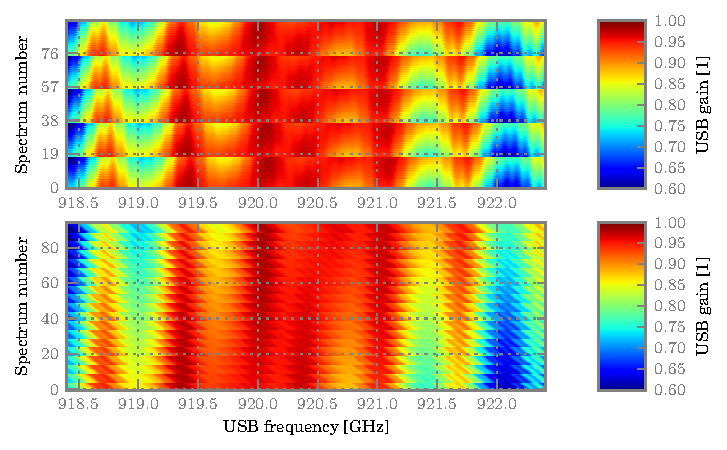
\includegraphics{87_interf_usG}
        \begin{minipage}{.82\linewidth}%
            \caption{USB sky target gain.}
            \label{fig:87_interf_usG}
        \end{minipage}
    \end{subfigure}%

    \begin{subfigure}[t]{\linewidth}
        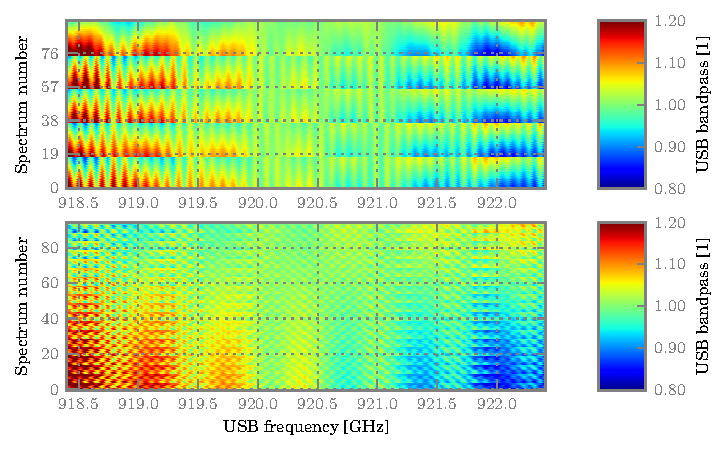
\includegraphics{87_interf_usB}
        \begin{minipage}{.82\linewidth}%
            \caption{USB sky target gain divided by bandpass.}
            \label{fig:87_interf_usB}
        \end{minipage}
    \end{subfigure}%

    \caption{
        Effect of the bandpass calibration on the gain.
        Each plot shows 95 \transition{CO}{8}{7} spectra stacked vertically, sorted
        either by LO then diplexer setting
            (\parensubref{fig:87_interf_usG} and
             \parensubref{fig:87_interf_usB} top)
        or     by diplexer then LO setting
            (\parensubref{fig:87_interf_usG} and
             \parensubref{fig:87_interf_usB} bottom).
        %
        The frequency-dependence of the diplexer causes the
        optical gain~\parensubref{fig:87_interf_usG} to be higher at the center of the
        spectra
        ($\text{red}=1$).
        %
        In~\parensubref{fig:87_interf_usB}, that gain is normalized
        ($\text{green}=1$)
        by being divided by the bandpass as measured from the hot and cold calibration
        loads.
        This approximation corrects the overall first-order effect of the diplexer but
        does not correct the effect of interferences.
        It even introduces short-period ripples that do not exist in~\parensubref{fig:87_interf_usG}.
    }
    \label{fig:87_interf_usGusB}
\end{figure}

\Cref{fig:87_00_00_sky_lsbusbsbr} shows the simulated optical gain for a spectrum of \transition{CO}{8}{7} when the chopper is pointed at the sky.
These curves present several interesting features.
\begin{itemize}[noitemsep,nolistsep]
    \item The widest feature is a bell-shaped (or U-shaped for the LO) curve that spans the entire bandwidth.  It is a product of the diplexer.  Even a perfect diplexer performs optimally at a single frequency.  Its gain degrades as we move away from this frequency and the diplexer starts coupling the mixer to the local oscillator instead.
    \item A ripple of period~$\approx \SI{650}{\mega\hertz}$.
    This matches the length of the cavities formed by the mixers and the rooftop mirrors.
    This is caused by imperfections in the grids (they leak power to the `wrong' polarization) and the rooftop mirrors (a small fraction of the incoming power is reflected without its polarization being rotated).
    \item A ripple of period~$\approx \SI{100}{\mega\hertz}$ that is stronger at the edge of the spectrum and weaker at the center.
    This ripple is caused by the LO--mixer cavity and is modulated by the LO coupling of the diplexer.
    \item A slope in the sideband gain ratio, which reveals a non-optimal diplexer tuning.
\end{itemize}

When the chopper points to the hot or cold calibration load, the non-zero reflectivity of this load introduces more cavities in the system, which creates additional ripples to the gain curves as shown in~\cref{fig:lsbusbsbr_hothot,fig:lsbusbsbr_coldcold}.
The lengths of the mixer--LO, mixer--hot-load and mixer--cold-load cavities are all close to~\SI{1.5}{\meter}, and therefore all produce ripples with periods between~\num{90} and \SI{100}{\mega\hertz}.

The USB gain of the signal for the sky pointing (\cref{fig:lsbusbsbr_skysky} center) is displayed on \cref{fig:87_interf_usG} for the 95 LO and diplexer settings of the \transition{CO}{8}{7} observation.
This illustrates the influence of the LO and diplexer setting on the intensity and the phase of the ripples affecting the line, which is located at~$\approx \SI{921.8}{\giga\hertz}$.

The bandpass calibration of HIFI involves dividing the signal measured on the sky by the signal measured on the calibration loads~(see \cref{sec:intensity_calibration}).
The USB gain of the sky signal divided by the bandpass, as measured on the hot and cold loads, is shown in~\cref{fig:87_interf_usB}.
The comparison of~\cref{fig:87_interf_usG} and~\cref{fig:87_interf_usB} clarifies the effect of the bandpass calibration: the bell-shaped curve caused by the diplexer (red region in the center of~\cref{fig:87_interf_usG}) is canceled by the bandpass division.
In reality, the bandpass corrects more than the variable optical gain, it also corrects the frequency-dependent gain of the IF chain (the electronics between the mixer and the detector).
The cost of the bandpass calibration is the injection into the spectrum of the ripples created by interferences in the mixer--load cavities.

In order to produce these models, we have to assume values for the coefficients of reflection and transmission of the various networks of the system.
In particular, we set the reflectivity of the calibration loads to~\SI{1}{\percent} in power and that of the LO to~\SI{5}{\percent}.
The mixer reflectivity depends on the polarization: it is low in the polarization that it couples but high in the other; we choose \SI{1}{\percent} and \SI{100}{\percent}.
The wires of the grids have a radius of~\SI{1}{\micro\meter} and are separated (axis-to-axis) by~\SI{4}{\micro\meter}; their conductivity is set to~\SI{e7}{\siemens\per\meter}, the order of the conductivity of aluminum.
We assume that~\SI{2}{\percent} of the power incident on the rooftop mirrors is reflected without its polarization rotated.
Finally, we set the LO attenuation to~\SI{-6}{\decibel}.
These values are estimations based on the knowledge of HIFI's optical design~\parencite[][for example]{jellema2003csa}, instrument test results and experimentations with previous models (see~\cref{sec:chapter4}).

Several parameters have not been included in our simulation.
In particular, the phase of the reflection coefficients.
The reflection coefficients of the mixers and local oscillator are likely to have an imaginary part which may depend on the LO~frequency: they are neither perfect conductors not perfect dielectrics.
The electronics of the local oscillator requires different settings for different LO~frequencies; which change the properties of the diode on which the electromagnetic wave reflects.
Likewise, each LO setting pumps the mixers with a specific power level and we can expect the surface of a mixer to reflect differently according to its pumping.
If these imaginary parts vary quickly with frequency, then we can expect the phase and the periods of the corresponding ripples to change in accordingly.


%#############################################################################
\FloatBarrier
\section{Observation}

We scheduled two observations of S140 IRS1 with HIFI.
They are available in the Herschel Science Archive~\parencite{herschelsciencearchive2015} under the following observation identifiers (``obsid''):
\begin{itemize}[noitemsep,nolistsep]
    \item \transition{CO}{8}{7}, obsid 0x50015e1d;
    \item \transition{CO}{9}{8}, obsid 0x50015d89.
\end{itemize}
These observations can be retrieved with HIPE~\parencite{ott2010herschel}, the data processing system and user front-end of HCSS
(Herschel Common Software System, \textcite{riedinger2009making})%
\footnote{
    HCSS and HIPE are joint developments by the Herschel Science Ground Segment Consortium, consisting of ESA, the NASA Herschel Science Center, and the HIFI, PACS and SPIRE consortia.
}%
.

A non-standard observing mode, based on the standard ``dual beam switch spectral scan'', was developped specifically for this observation.
The standard observing modes of HIFI are described in~\textcite{hifiobserversmanual}.

``Dual beam switch'' refers to the choice of the reference source used for subtracting the background radiation: two positions on the sky.
\Cref{tab:on_off_positions} lists the positions of the On and the two Off.
The On position is centered on~IRS1.
The two Off positions are~\SI{3}{\arcmin} away from IRS1 in the north-west and south-east directions.
We assume that there is no \transition{CO}{8}{7} or \transition{CO}{9}{8} emission in the Off positions.
First, these transition have upper-level energies well above the kinetic temperature of the cloud at these positions.
Second, both positions are shielded from the UV radiation emitted by HD~211880 and the three infrared sources.

``Spectral scan'' means that each observation contains spectra taken at different local oscillator frequencies.
Changing the LO~frequency is one way to modulate the interferences in HIFI.

The non-standard aspect of our observing mode is that, for each local oscillator frequency, there are 19 different diplexer settings instead of a single one.
This allows us to modulate interferences for a given LO~frequency.

\Cref{tab:los_and_dacs} lists the five LO~frequencies and the nineteen diplexer actuator currents used for each transition.
Each transition is observed 95~times.
In principle, each LO~frequency corresponds to one and only one ideal diplexer setting
(see~\cref{sec:hifi_diplexers_interferences}).
Consequently, most of the LO/diplexer combinations of our observation are not ideal.
The closest matches for each \ce{CO} transition are indicated by the gray background in~\cref{tab:los_and_dacs}.

\begin{table}[b]
%dataset 11
%334.79607197925145  63.3615103585033      22h19m11.05s  63º21'41.43729"
%334.8260678609779   63.31298895703982     22h19m18.26s  63º18'46.76025"
%334.8259243886195   63.31303201092469     22h19m18.22s  63º18'46.91524"
%334.7956101137214   63.361555679611314    22h19m10.95s  63º21'41.60045"
%
%dataset 15
%334.8263617781845   63.31300182715389     22h19m18.32s  63º18'46.80658"
%334.8563340071168   63.26442869962732     22h19m25.52s  63º15'51.94332"
%334.85622353208436  63.26443044144398     22h19m25.49s  63º15'51.94959"
%334.82593558348606  63.312952587111134    22h19m18.22s  63º18'46.62931"
    \centering
    \begin{tabular}{lll}
        \toprule
        pointing  & right ascension & declination \\
        \midrule
        Off left  & $22^\text{h}19^\text{m}11.0^\text{s}$ & \ang{63;21;41.5}\\
        On        & $22^\text{h}19^\text{m}18.2^\text{s}$ & \ang{63;18;46.8}\\
        Off right & $22^\text{h}19^\text{m}25.5^\text{s}$ & \ang{63;15;51.9}\\
        \bottomrule
    \end{tabular}
    \caption{Equatorial coordinates (mean equinox J2000) of the three pointings used in our observations.}
    \label{tab:on_off_positions}
\end{table}

\begin{table}[b]
    \centering
    \begin{tabularx}{\textwidth}{Xrrrrr}
        \toprule
        transition & \multicolumn{5}{c}{LO~frequencies [\si{\giga\hertz}]} \\
        \midrule
        \Jlevel{8}{7} &  914.4045 &  914.4225 &  914.4450 &                     914.4630 &  \cellcolor{gray!40}914.4810 \\
        \Jlevel{9}{8} & 1029.4830 & 1029.5010 & 1029.5190 & \cellcolor{gray!40}1029.5415 &                    1029.5595 \\
        \bottomrule
        \toprule
        transition & \multicolumn{5}{c}{horizontal diplexer actuator currents [\si{\milli\ampere}]} \\
        \midrule
        \multirow{4}{*}{\Jlevel{8}{7}}
        & 0.503 & 0.499 & 0.493 & 0.488 & 0.481 \\
        & 0.476 & 0.471 & 0.465 & 0.458 & 0.453 \\
        & 0.447 & \cellcolor{gray!40}0.442 & 0.435 & 0.430 & 0.425 \\
        & 0.419 & 0.412 & 0.407 & 0.401 & \\
        \midrule
        \multirow{4}{*}{\Jlevel{9}{8}}
        & 1.336 & 1.332 & 1.325 & 1.318 & 1.313 \\
        & 1.306 & 1.300 & 1.293 & 1.288 & 1.281 \\
        & \cellcolor{gray!40}1.275 & 1.269 & 1.263 & 1.256 & 1.251 \\
        & 1.244 & 1.237 & 1.232 & 1.225 & \\
        \bottomrule
    \end{tabularx}
    \caption{
        Local oscillator frequencies and diplexer actuator currents used for each \ce{CO} transition.
        For each LO~frequency there exist an optimal diplexer current;
        in our observation, the LO and diplexer are often mismatched.
        The cells in gray indicate the values that are the closest to an ideal match.
    }
    \label{tab:los_and_dacs}
\end{table}

The 19 diplexer settings create optical pathlength differences in the interferometer of $\pm1~\text{wavelength}$ around the nominal value.

The 5 LO~frequencies are very close to each other.
They are separated by only \num{18.0} or \SI{22.5}{\mega\hertz}
which corresponds to the smallest possible steps of the tunable LO~frequencies.
For each transition, the LO~frequencies cover a range of~\SI{76.5}{\mega\hertz}.
We have chosen this range in order to sample the interferences created by the mixer--LO, mixer--hot-load and mixer--cold-load cavities.

The LO~frequencies are chosen so that the lines always appear in the upper sideband.
Furthermore, the lines are not placed in the center of the spectra but close to the edge, where the effect of the interferences is stronger.

A hot-cold measurement is taken for each instrumental configuration: each spectrum is calibrated with its own bandpass, measured with the corresponding LO~frequency and diplexer actuator current.





%#############################################################################
\FloatBarrier
\section{Data reduction}
\label{sec:s140_data_reduction}
Our study focuses on spectra provided by the WBS-H backend of HIFI: the acousto-optic WideBand Spectrometer sensitive to the horizontal polarization.
The WBS allows us to see the full bandwidth of the mixers while still resolving our lines.
We choose the horizontal polarization because its system temperature is lower: in Bands~3 and 4, the V mixer is slightly under-pumped and therefore less sensitive (see~\cref{tab:chapter5_tsys}).

\begin{table}
    \centering
    \begin{tabular}{ccc}
        \toprule
        LO~frequency [\si{\giga\hertz}] &
        $T_\text{sys, H}$ [\si{\kelvin}] &
        $T_\text{sys, V}$ [\si{\kelvin}]\\
        \midrule
        \num{914.46}   &   225   &   275 \\ % Tsys_1342192329 0x50003ac9
        \num{1029.52}  &   325   &   425 \\ % Tsys_1342191601 0x500037f1
        \bottomrule
    \end{tabular}
    \caption{
        System temperatures of the H and V mixers at the LO~frequencies of our observation, at the intermediate frequency of our line.
        Source: Herschel Science Archive, calibration observations 0x50003ac9
        and 0x500037f1.
    }
    \label{tab:chapter5_tsys}
\end{table}


%=============================================================================

\subsection{Custom pipeline}

Because the observing mode is not standard, one assumption of the default HIFI data reduction pipeline~\parencite{hifiobserversmanual} is not valid.
It is necessary to rerun the pipeline from Level-0 (raw telemetry) to Level-2 (calibrated spectra) with a custom configuration:
the ``doAverage'' task of the pipeline must be disabled.
Leaving it enabled (the default) averages the spectra taken with different diplexer settings, which is not what we want.



%=============================================================================

\subsection{Temperature scale}
The HIFI pipeline produces spectra with a power scale expressed as an antenna temperature~$T_\text{a}$
(see~\textcite{kutner1981recommendations} for details regarding the various temperature scales used in radioastronomy).
That temperature scale is suitable for extended sources as it assumes that the emission of the source is received not only in the main beam but also in the side lobes.

\begin{figure}
    \centering
    \includegraphics{87_00_00_tmb}
    \caption{
        Spectrum of \transition{CO}{8}{7} shown over its full \SI{4}{\giga\hertz} bandwidth.
    }
    \label{fig:co98_full_bandwidth}
\end{figure}

    % a = 1.22 lambda / D with D = 3.5 and lambda = c_0 / f.
    %   fl =  921.7997000e9 => ll = 0.000325225163341 => al = 0.000113364199793 rad
    %   fu = 1036.9123930e9 => lu = 0.000289120334585 => au = 0.000100779088056 rad
    % To convert to second: sec = 3600*180/pi = 206264.80624709636
    %   al * sec = 23.3830447056765
    %   au * sec = 20.78717907152951
    % To convert to diameter, multiply by distance L = 746 * parsec. (+/-4%)
    % With parsec = 3.086e16 meter
    %   al * L = 2.60982072739e+15 m  (Don't forget, 4% precision)
    %   au * L = 2.32009182242e+15 m
    % Warning, these are diameters.
    % Evgenia uses an inner radius of 2e14 cm = 2e12 m.
    % Her outer radius is 1500 times the inner radius, so 3e15.
    % That does put us pretty much exactly in that area.
    % There, she says that her density gradient for IRS1 goes as r^-0.4, calls it "mild".

Our sources are probably much smaller than our beam size and an absolute calibration of their intensity requires knowing their apparent diameter.
This does not matter for measuring our line ratios:
if the lines originate from the same regions, the ratio cancels their apparent diameter.
For our purpose, the main-beam temperature scale ($T_\text{mb}$) is appropriate.
It assumes that the source fills the main beam but not the sidelobes.

The antenna and main-beam temperatures are related by $T_\text{mb} = T_\text{a} / \eta_\text{mb}$ where $\eta_\text{mb}$ is the main-beam efficiency.
\Textcite{AA_537_A17} provides a table of main-beam efficiencies for each HIFI band.
In addition, each HIFI data product present in the Herschel Science Archive contains a table of main-beam efficiencies that is more accurate and up-to-date.
Interpolating this table for the relevent LO frequencies yields
$\eta_\text{mb}=\num{0.744}$ for \transition{CO}{8}{7} and $\eta_\text{mb}=\num{0.740}$ for \transition{CO}{9}{8}.
\Cref{fig:co98_full_bandwidth} shows one of the 95 spectra of \transition{CO}{8}{7} on the $T_\text{mb}$~scale.

For both transitions, the \ce{CO} line is always relatively narrow ($\approx \SI{100}{\mega\hertz}$) compared to the instantaneous bandwidth of the instrument (\SI{4}{\giga\hertz}), and in the rest of this chapter we will often zoom in on the line.
The 195 spectra that we study are all very similar to the one shown in~\cref{fig:co98_full_bandwidth}.
The spectra of both transitions typically feature:
\begin{itemize}[noitemsep,nolistsep]
    \item a horizontal baseline of $\SI{1.8}{\kelvin}$ due to the difference of black-body emission at the On and the Off positions in the sky,
    \item a noise of standard deviation $\SI{0.2}{\kelvin}$ slightly stronger at the edges of the spectra than in the center.
    \item an emission line of~$\approx \SI{30}{\kelvin}$ located in the highest-frequency quarter of the spectrum.
\end{itemize}



%=============================================================================

\subsection{Diplexer mis-tuning correction}

%-----------------------------------------------------------------------------
\subsubsection{Motivation}
For our experiment, we use the diplexer as a way of modulating the interferences inside the optics of HIFI.
However, for each LO~frequency there exist one and only one diplexer tuning that guarantees ideal couplings and a balanced sideband gain ratio.
By mis-tuning the diplexer, we do modulate the interferences, but we also deteriorate the sideband ratio in a way that is irrelevant for our study.
In this section, we describe how we correct for this degradation of the sideband ratio.

The diplexer units are modules of the HIFI focal plane unit that are used in Bands~3, 4, 6, and 7 for the LO injection~\parencite{jackson2002hifi}.
They are used to align the polarization of the sky and LO signals so that the mixers, which are sensitive to one polarization only, can couple to both optimally.




In normal operations, the diplexer actuator current is adjusted to the LO~frequency by interpolation of a look-up table.
For our observations, we bypass this process and set the diplexer actuator current ourselves.
As a result, the diplexer is not optimally tuned.
This is illustrated in~\cref{fig:diplexer_0503}, for which the diplexer actuator current of~\SI{0.503}{\milli\ampere} for a LO~frequency of~\SI{914.4045}{\giga\hertz} results in an arm length mis-tuned by \SI{158}{\micro\meter}, approximately half a wavelength.
The coupling is not symmetrical (top plot) and the sideband ratio does not equal \num{0.5} everywhere.
This distorts the line profile.
We must correct for it.

\begin{figure}
    \centering
    \includegraphics{diplexer_coupling_0503}
    \caption*{
        Coupling of the mixer by the LO and the sky for a mis-tuned diplexer.
        In this specific case, the coupling is shifted \SI{53}{\mega\hertz} to the left of its optimal position.
    }
    \bigskip
    \includegraphics{diplexer_sbr_0503}
    \caption*{
        Sideband ratio of the mixer--sky coupling for a mis-tuned diplexer.
        The left part of the spectrum is USB-dominated, the right part is LSB-dominated.
        The intensity of the \transition{CO}{8}{7} line is underestimated by about~\SI{10}{\percent}.
    }
    \caption{
    Model of the coupling and the sideband ratio for a mis-tuned diplexer.
    The green vertical lines show the rest frequency of the \transition{CO}{8}{7} transition.
    The LO~frequency is~\SI{914.4045}{\giga\hertz}.
    The difference in length of the two arms of the diplexer is~\SI{12.3826}{\milli\meter}.
    }
    \label{fig:diplexer_0503}
\end{figure}

%-----------------------------------------------------------------------------
\subsubsection{Correcting for the diplexer mis-tuning}
We start by assuming that the diplexer gain is the same for the four pointings of the observation (Source or On, Reference or Off, Hot, Cold):
$G_L$ for the LSB frequency and $G_U$ for the USB frequency that contribute to the same intermediate frequency.
These gains affect the powers from
the source ($S_L$ and $S_U$),
the reference ($R_L$ and $R_U$),
the hot ($H_L$ and $H_U$) and
the cold ($C_L$ and $C_U$).
The calibration equation of HIFI produces $T_\text{mb}$ from the measured powers, which are distorted by the diplexer:
\begin{equation}
    T_\text{mb}
    =
    \Delta T
    \frac{
        (G_L S_L + G_U S_U) - (G_L R_L + G_U R_U)
    }{
        (G_L H_L + G_U H_U) - (G_L C_L + G_U C_U)
    }\text{.}
\end{equation}
In this equation, $\Delta T$ is a scaling factor converting the dimensionless ratio to a temperature.
Without loss of generality, let us assume $R_L = R_U = 0$: there is no emission from the Off.

%...................................................................
\paragraph{Step 1: find the continuum.}
We assume that parts of the spectrum show only a continuum emission and no line.
Furthermore, we assume that the amplitude of the continuum is constant.
The signal in both sidebands equals this constant: $S_L = S_U = B$.
We get
\begin{equation}
    T_\text{mb}
    =
    \Delta T
    \frac{
        (G_L + G_U) B
    }{
        (G_L H_L + G_U H_U) - (G_L C_L + G_U C_U)
    }
\end{equation}
In this equation, $G_L$ and $G_U$ are known: we calculate them from a known diplexer displacement with~\cref{eq:diplexer_coupling_model}.
We also know $H$ and $C$, the emission from the hot and cold calibration loads: we know their physical temperature $T_h$ and $T_c$, their coupling coefficient and Planck's law.
Finally, $\Delta T = T_h - T_c$ is known as well.
We can therefore easily solve this equation for $B$.
Each channel of the spectrum gives a different value for $B$, but if the spectrum is flat, these values are very close to each other.
We simply take their average.

%...................................................................
\paragraph{Step 2: solve for the line.}
We know that our emission lines are located in the upper sideband.
The lower sideband sees only the continuum.
With $B$ the continuum intensity that we just calculated and $L$ the intensity of the line, we have
\begin{equation}
    T_\text{mb}
    =
    \Delta T
    \frac{
        G_L B + G_U (B + L)
    }{
        (G_L H_L + G_U H_U) - (G_L C_L + G_U C_U)
    }\text{,}
\end{equation}
which we solve for $L$.

Note: this equation cannot make the difference between the noise and the astronomical signal.
Any deviation from the baseline enters~$L$.
The intensity of the noise and the line are both `corrected' equally.

%...................................................................
\paragraph{Step 3: recalibrate.}
The previous steps give us the intensities of the continuum and the line before being distorted by the diplexer mis-tuning.
We can choose whether we re-introduce the continuum or if we leave it out.
The two situations are described by the equations
\begin{align}
    T_\text{mb}'
    &=
    \Delta T
    \frac{B+L}{(H_L + H_U) - (C_L + C_U)} \text{\quad with continuum and}
    \\
    T_\text{mb}''
    &=
    \Delta T
    \frac{L}{(H_L + H_U) - (C_L + C_U)} \text{\quad with the line only.}
\end{align}

In the rest of this chapter, we use the $T_\text{mb}''$ scale.

%-----------------------------------------------------------------------------
\subsubsection{Result of the diplexer mis-tuning correction}
\Cref{fig:diplexer_correction} shows the result of correcting the sideband imbalance with this simple method.
The bottom plot for each transition shows the line only, the continuum is removed.

\begin{figure}
    \centering
    \begin{subfigure}[b]{\textwidth}
        \centering
        \includegraphics{correction_87}
        \vspace{-.8em}
        \caption{\transition{CO}{8}{7} spectra before and after sideband correction.}
    \end{subfigure}
    \\
    \bigskip
    \begin{subfigure}[b]{\textwidth}
        \centering
        \includegraphics{correction_98}
        \vspace{-.8em}
        \caption{\transition{CO}{9}{8} spectra before and after sideband correction.}
    \end{subfigure}
    \caption{
        Correction of the sideband imbalance due to mis-tuning the mixer.
    }
    \label{fig:diplexer_correction}
\end{figure}


For both transitions, the spread of the peak intensity is considerably reduced.
\begin{table}
    %87 Before correction 31.5146912873 +/- 1.31935031215
    %87 After  correction 32.3597611286 +/- 0.27093631469
    %98 Before correction 31.2396155249 +/- 1.49534099289
    %98 After  correction 32.7454980568 +/- 0.448444802488
    \centering
    \begin{tabular}{ccc}
        \toprule
        transition & before correction & after correction \\
        \midrule
        \transition{CO}{8}{7} & $\num{31.5} \pm \SI{1.3}{\kelvin}$ &
                                $\num{32.4} \pm \SI{0.3}{\kelvin}$\\
        \transition{CO}{9}{8} & $\num{31.2} \pm \SI{1.5}{\kelvin}$ &
                                $\num{32.7} \pm \SI{0.5}{\kelvin}$\\ 
        \bottomrule
    \end{tabular}
    \caption{Peak intensities before and after correcting for the diplexer mis-tuning.}
\end{table}

Any residual spread is due to either thermal noise, imperfections in the diplexers and interferences in the optics.





%#############################################################################
%\FloatBarrier
\section{Noise simulations}
\label{sec:noise_simulations}
We wish to quantify the influence of the thermal noise on the line profiles.
We model the noise seen on HIFI observations and use that model to generate synthetic spectra.
This mimics an observation in which the same source is observed many times with a fixed LO and diplexer settings.
These synthetic spectra differ only by their noise, not by variations in the optical gain.
We proceed in three steps.
First, construct an ideal spectrum for each transition.
Then, model the thermal noise affecting the real spectra.
Finally, apply the modeled thermal noise to the ideal spectra.



%=============================================================================

\subsection{Ideal spectra}
For our ideal hopefully-noiseless spectra, we choose to average the 95~spectra of each transition.
The averaged spectra are shown in~\cref{fig:corrected_averaged}.
We do not claim that these averaged spectra are closer to the astronomical reality than any individual spectrum: averaging reduces the noise but may leave systematic instrumental effects in the bandpass.

By averaging, we reduce the noise by a factor~$\sqrt{95} \approx 10$ but we do not completely eliminate it.

\begin{figure}
    \centering
    \begin{subfigure}[b]{\textwidth}
        \centering
        \includegraphics{87_avera_corrected_tmb}
        \vspace{-.8em}
        \caption{Average of the 95 \transition{CO}{8}{7} diplexer-corrected spectra.}
    \end{subfigure}
    \\
    \begin{subfigure}[b]{\textwidth}
        \centering
        \includegraphics{98_avera_corrected_tmb}
        \vspace{-.8em}
        \caption{Average of the 95 \transition{CO}{9}{8} diplexer-corrected spectra.}
    \end{subfigure}
    \caption{Average of the spectra corrected for diplexer mix-tuning.}
    \label{fig:corrected_averaged}
\end{figure}

%=============================================================================
\subsection{Thermal noise modeling}
We model the thermal noise with a polynomial in Fourier space.

Using Fourier Transforms to analyze a signal is relatively trivial: signals have an analytic expression, they can be written as function of time or frequency.
The noise does not have an analytic expression: it is a stochastic process that can be described only in statistical terms such as variance.
The noise is not visible on the spectra that we measured, what we have is one very specific instance of an inherently random process, one single state taken out of the infinite%
\footnote{Infinite if we assume that the probability distribution is continuous, but quantum processes ultimately limit this to a finite, albeit overwhelmingly large, state space.}
state space of the system.
Fourier analysis treats that particular state as if it were signal.
We must estimate the properties of the stochastic process from that specific sequence.

The power of a stochastic process is, in statistical term, its variance.
The variance can be a function of frequency, for example the ``pink noise'' or the ``$1/f$ noise'' have different variances at different frequencies.
These can be represented on a ``periodogram'', a graph that plots the ``power spectral density'' (PSD) as a function of a frequency/period/scale.
If we consider a time-varying electric potential in volt,
the unit of the PSD of its noise is \si{\volt\squared\second} or \si{\volt\squared\per\hertz}.
In our case, the data is a temperature as a function of frequency;
the PSD of its noise is in~\si{\kelvin\squared\hertz}.
The estimation of the PSD from a signal is a subtle matter, subject of a significant volume of literature (i.e.\ \textcite{burg1967maximum,percival1993spectral}).

In our situation, an accurate estimation of the PSD is not required.
Our goal is to generate 190~synthetic spectra which present 190~particular noise states.
It is sufficient to know these 190~particular states, one does not need to model accurately the entire state space.
We only need the Fourier Transform of our synthetic spectra to match that of the real data.

Taking spectra of spectra can lead to a confusing terminology.
Furthermore there are at least four Fourier spectra of interest for a single direct spectrum.
\Cref{tab:direct_fourier} clarifies the terminology used in this section.

\begin{table}
    \centering
    \begin{tabular}{llcll}
    \toprule
    \multicolumn{5}{l}{Direct spectrum}\\
    \midrule
    $x$-axis & frequency   & $f$ & $\mathbb{R}$ & [\si{\hertz}]\\
    $y$-axis & temperature & $T$ & $\mathbb{R}$ & [\si{\kelvin}]\\
    \bottomrule
    \\
    \toprule
    \multicolumn{5}{l}{Fourier spectra}\\
    \midrule
    $x$-axis & reciprocal frequency & $t$         & $\mathbb{R}$ & [\si{\per\hertz}]\\
    $y$-axis & complex spectrum     & $z$         & $\mathbb{C}$ & [\si{\kelvin}]   \\
             & phase spectrum       & $\arg(z)$   & $\mathbb{R}$ & [\si{\radian}]   \\
             & amplitude spectrum   & $\abs{z}$   & $\mathbb{R}$ & [\si{\kelvin}]   \\
             & normalized-amplitude spectrum & $\abs{z}/n$& $\mathbb{R}$ & [\si{\kelvin}]   \\
    \bottomrule
    \end{tabular}
    \caption{Definitions and units used in Direct and Fourier space.}
    \label{tab:direct_fourier}
\end{table}

Normalized amplitudes allow the comparison of spectra taken with different sampling rates~$\delta f$ and/or different bandwidths~$\Delta f = n \delta f$ (with $n$ the number of channels in the spectrum) by multiplying them by $\delta f / \Delta f = 1/n$.
We use amplitude and normalized-amplitude spectra where necessary:
amplitude spectra can be converted back to direct space;
normalized-amplitude spectra can be compared.

We do not analyze our noise with energy density or power density spectra.
Energy and power density spectra require raising the amplitude to the power 2, which enhances the contrast between the high- and low-amplitude parts of the spectra.
From our experiments, we determined that fitting the energy or power spectrum requires a polynomial of order $>10$ while an order-6 is sufficient to fit the amplitude.
Furthermore, we need our final result in amplitude so that it can be converted back to the direct domain with an inverse-DFT, making the round-trip between amplitude and power unnecessary.

It is easier to measure the noise on the the baseline than on the lines.
The lines are located in the high-frequency half of the direct spectra (see~\cref{fig:co98_full_bandwidth}), therefore we take the Fourier Transform of the lower-frequency half.
We remove any continuum level from the direct spectrum to minimize the artifacts created by the Discrete Fourier Transform (DFT) algorithm.

Finally, we do not apodize our direct spectra with a window.
Windowing is recommended to reduce the ``leakage'' caused by the truncation of the direct data when we need to accurately quantify the amplitude/energy/power at a given frequency on a correct scale.
We are not interested in the absolute levels of amplitude/energy/power;
we are satisfied when the normalized-amplitude of the synthetic spectrum matches that of the real spectrum, leakage included.

%-----------------------------------------------------------------------------
\subsubsection{Noise model of the ideal spectra}

The noise spectra of our ideal spectra are shown in \cref{fig:noise_model_87}(a)
and~\cref{fig:noise_model_98}(a).
The normalized amplitude is in black and its polynomial model in red.

The small plots inside the larger ones zoom into the region in which we expect interferences to leave traces.
Their $x$-axis gives the period of the ripples caused by interferences.
These spectra peak at two periods:
$\approx\SI{90}{\mega\hertz}$ and $\approx\SI{600}{\mega\hertz}$.

The $\SI{90}{\mega\hertz}$ ripple originates from the mixer--LO, mixer--hot-load and/or mixer--cold load cavities.
These cannot be distinguished at this resolution.

The $\SI{600}{\mega\hertz}$ ripple comes from the mixer--rooftop-mirrors cavities.

The averaging process by which we create the ideal spectra retains these two ripples.
This indicates that their phase varies little over the 95~spectra involved in the average:
they interfere constructively.

The polynomial model ignores these peaks of amplitude density: these regions are deliberately masked before fitting the polynomial.
Indeed, the polynomial must follow the thermal noise only and these peaks are not of thermal origin.

%-----------------------------------------------------------------------------
\subsubsection{Noise model of the real spectra}
\label{sec:noise_model_of_the_real_spectra}

The main sources of noise in HIFI are the mixer, the local oscillator and the telescope dish.
The diplexer setting has an influence on how much LO noise the mixer receives but we calculate that our diplexer settings should change that value by less than one percent.
The LO is responsible for less than~\SI{10}{\percent} of the total system temperature.
We conclude that, for modeling our noise, we should not attempt to ``correct'' its intensity for diplexer mis-tuning.
The noise measured on the original spectra is the correct one.

In this step, we do not take the DFT of an average but the average of DFTs.
Indeed, we do not wish to attenuate the noise of the real spectra by averaging them.
However, we wish to reduce the uncertainty of our polynomial model, which we can achieve by averaging the DFTs.

The normalized-amplitude spectra of the baseline, and their polynomial models, are presented in~%
\cref{fig:noise_model_87}(b) and~\cref{fig:noise_model_98}(b).

The two peaks at~\SI{90}{\mega\hertz} and~\SI{600}{\mega\hertz} that are present on the ideal spectra are also visible on these real spectra.
These peaks are less well-defined because the noise is stronger.

A new feature appears on these spectra: a peak at~\SI{875}{\per\giga\hertz} which corresponds to a period of~$\approx\SI{1.14}{\mega\hertz}$.
This peak is visible on the average of DFTs but not on the DFT of averages.
This indicates that the corresponding ripple interferes destructively during the averaging: its phase changes a lot.
It is unlikely that this feature corresponds to a cavity: the cavity would need to be~\SI{130}{\meter}-long.
We have not determined its origin.
Possible explanations include
\begin{itemize}[noitemsep,nolistsep]
    \item An artifact of the sampling of the WBS:
the even and odd channels of the WBS CCD have different levels of dark currents.
These channels are separated by about~\SI{0.5}{\mega\hertz} and an imperfect calibration of these dark currents could generate a~\SI{1}{\mega\hertz}-period ripple.
    \item An artifact of the regridding done by the HIFI pipeline:
the spectra produced by the WBS have an irregular frequency axis.
The pipeline resamples it onto a regular grid.
This might produce some artifacts at the scale of the channel spacing (\SI{0.5}{\mega\hertz}) or the channel resolution~\SI{1.1}{\mega\hertz}.
\end{itemize}
In any case, this feature is non-thermal and its region is masked during the fit of our polynomial model.

\begin{figure}[p]
    \centering
    \begin{subfigure}[b]{\textwidth}
        \centering
        \includegraphics{noise_dft_87_correctedavg}
        \vspace{-.8em}
        \caption{Noise of the average of 95 \transition{CO}{8}{7} diplexer-corrected spectra.}
        %\label{fig:noise_dft_87_correctedavg}
    \end{subfigure}
    \\
    \bigskip
    \begin{subfigure}[b]{\textwidth}
        \centering
        \includegraphics{noise_dft_87_original}
        \vspace{-.8em}
        \caption{Averaged noise of 95 \transition{CO}{8}{7} original spectra.}
        %\label{fig:noise_dft_87_original}
    \end{subfigure}
    \\
    \bigskip
    \begin{subfigure}[b]{\textwidth}
        \centering
        \includegraphics{noise_dft_87_noisy}
        \vspace{-.8em}
        \caption{Averaged noise of 95 \transition{CO}{8}{7} synthetic noisy spectra.}
        %\label{fig:noise_dft_87_noisy}
    \end{subfigure}
    \caption{Noise modeling of the~\transition{CO}{8}{7} spectra.}
    \label{fig:noise_model_87}
\end{figure}

\begin{figure}[p]
    \centering
    \begin{subfigure}[b]{\textwidth}
        \centering
        \includegraphics{noise_dft_98_correctedavg}
        \vspace{-.8em}
        \caption{Noise of the average of 95 \transition{CO}{9}{8} diplexer-corrected spectra.}
    \end{subfigure}
    \\
    \bigskip
    \begin{subfigure}[b]{\textwidth}
        \centering
        \includegraphics{noise_dft_98_original}
        \vspace{-.8em}
        \caption{Averaged noise of 95 \transition{CO}{9}{8} original spectra.}
    \end{subfigure}
    \\
    \bigskip
    \begin{subfigure}[b]{\textwidth}
        \centering
        \includegraphics{noise_dft_98_noisy}
        \vspace{-.8em}
        \caption{Averaged noise of 95 \transition{CO}{9}{8} synthetic noisy spectra.}
    \end{subfigure}
    \caption{Noise modeling of the~\transition{CO}{9}{8} spectra.}
    \label{fig:noise_model_98}
\end{figure}


%=============================================================================
\FloatBarrier
\subsection{Synthesis of the thermal noise}
We generate artificial noise in the Fourier space and convert it to Direct space with an inverse Discrete Fourier Transform via a technique called ``phase randomization'' \parencite{yamada1991orthonormal}.

The complex spectrum of our synthetic noise is an array of complex numbers $z=\rho \exp(i \theta)$.
The array $\rho=\abs{z}$ is an amplitude spectrum.
The array $\theta=\arg(z)$ is a phase spectrum.

A polynomial model describes a normalized-amplitude spectrum $\abs{z}/n$ with $n$ the number of channels.
Multiplying that model by the appropriate $n$ gives a amplitude spectrum $\rho$.

We use a pseudo-random number generator with a uniform distribution to generate a phase spectrum with values of $\theta \in [0, 2\pi[$.

We call $A$ the noise model of the ideal spectra and $B$ the noise model of the real spectra.
The noise that we need to add to the ideal spectra in order to bring them to $A$ is not
$C=A-B$: noise adds in power, not in intensity.
The addition in power ($C=\sqrt{A^2-B^2}$) does not produce synthetic spectra with a noise of $A$ either: the randomness is too high (or the number of channels too low).
Instead, we determine $C$ by fitting it; the objective function generates hundreds of synthetic spectra at each iteration until the normalized-amplitude spectrum of their noise matches~$A$.

The average noise of our 190 synthetic spectra (95 per transition) can be seen
in~\cref{fig:noise_model_87}(c) and~\cref{fig:noise_model_98}(c).
As desired, it is very similar to the noise observed on the real spectra (middle plots).
In addition, the peaks present on the top and middle spectra have all but disappeared.

We have created synthetic spectra that mimic the noise seen on the real spectra without including their systematic variability.
We can now analyze the line profiles of the real and synthetic spectra.




%#############################################################################
\FloatBarrier
\section{Line profile analysis}



We begin our analysis by measuring the various components constituting the lines profiles of \transition{CO}{8}{7} and \transition{CO}{9}{8} seen by HIFI in S140 IRS1.

We perform the same analysis with two sets of spectra:
the real HIFI spectra corrected for diplexer-mis-tuning (\cref{sec:s140_data_reduction})
and
the synthetic spectra that simulate an observation that is affected only by thermal noise (\cref{sec:noise_simulations}).


%=============================================================================
\FloatBarrier
\subsection{Gaussian fit of the spectra}
\label{sec:chp5_gaussian_model}
\Cref{fig:spectra_transitions} shows the real diplexer-corrected spectra for an arbitrary LO and diplexer setting, one for each transition.
Superimposed on these spectra are the various components of a Gaussian fit.

\begin{figure}
    \centering
    \begin{subfigure}[b]{\textwidth}
        \includegraphics{87_00_00_corrected}
        \vspace{-.8em}
        \caption{\transition{CO}{8}{7}, rest frequency \SI{ 921.7997000}{\giga\hertz}.}
    \end{subfigure}
    \\
    \bigskip
    \begin{subfigure}[b]{\textwidth}
        \includegraphics{98_00_00_corrected}
        \vspace{-.8em}
        \caption{\transition{CO}{9}{8}, rest frequency \SI{1036.9123930}{\giga\hertz}.}
    \end{subfigure}
    \caption{
        HIFI WBS-H spectra of S140 IRS1 for \transition{CO}{8}{7} and \transition{CO}{9}{8}.
        For each transition, the the top plot shows the data in black and the model (simple Gaussian fit) in color, where the full model is the sum of the others; and the bottom plot shows the difference between the data and the full model.
    }
    \label{fig:spectra_transitions}
\end{figure}

\begin{samepage}
We fit three or four components with Gaussian functions:
\begin{itemize}[noitemsep,nolistsep]
    \item a constant horizontal continuum ($c$),
    \item a narrow Gaussian for the core emission ($a_0$, $v_0$, $\sigma_0$),
    \item a broad Gaussian for the outflow emission ($a_1$, $v_1$, $\sigma_1$),
    \item and optionally a third negative Gaussian for a self-absorption
     ($a_2$, $v_2$, $\sigma_2$).
\end{itemize}
\end{samepage}
Both transitions show a self-absorption, but in the case \transition{CO}{9}{8} the self-absorption is barely visible in the noise, which makes it difficult to fit.
For each Gaussian function, $a$ is the amplitude, $v$ the mean and $\sigma$ the standard deviation.

%-----------------------------------------------------------------------------
\subsubsection{Core and outflow velocity}
The outflow is not as collimated as the jet that creates it; shocks, collisions and turbulence create a wide range of velocities inside the outflow.
In comparison, the velocities in the core are more homogeneous.
Through the Doppler effect, a larger velocity range translates into broader lines, which is why the outflow component (blue in~\cref{fig:spectra_transitions} is wider than the core component (in green).

The \ce{CO} lines of S140~IRS1 are blue-shifted;
the core moves towards us with a radial velocity of~\SI{-5}{\kilo\meter\per\second}.
The peak intensity of the outflow is on the blue side of the core: it approaches us at~\SI{-9}{\kilo\meter\per\second}, faster than the core does.
\Textcite{maud2013s140} measure a speed of~\SI{-25}{\kilo\meter\per\second} for the blue \transition{CO}{1}{0} outflow.
We justify the difference by the distance to the core.
Our high-$J$ lines are emitted near the core, the jet had little time to accelerate the \ce{CO} molecules.
On the other hand, the \transition{CO}{1}{0} outflow is observed much farther and has been accelerated by the jet much longer.

The line profiles do not show any evidence of a bimodal distribution of velocities as one could expect from a rotating disk seen edge-on.
We conclude that the emission that we observe does not originate (solely) from the accretion disk orbiting the young stellar object.

%-----------------------------------------------------------------------------
\subsubsection{Missing red outflow}
Since the outflow of IRS1 is bipolar, one would expect a second outflow line on the red side of the core.
The spectra do not show this second outflow component.
The emission of the red outflow
may be weaker due do different density and temperature conditions
or it may be absorbed by the dense circumstellar envelope before reaching the detector.

%-----------------------------------------------------------------------------
\subsubsection{Self-absorption}
The absorption feature seen at~$v_\text{LSR}=\SI{-9}{\kilo\meter\per\second}$ attests that \transition{CO}{8}{7} is not optically thin at all frequencies.
The absorption and outflow components have a similar velocity:
this is a case of self-absorption, in which the photons at the line wings have a smaller re-absorption probability than the photons at the line center.

%-----------------------------------------------------------------------------
\subsubsection{Structure of the residual}
The difference between the data and our fit (``residuals'' on the plots) shows some structure.
In particular, the blue wing of the line is systematically underestimated: the residual at~\SI{-25}{\kilo\meter\per\second} reaches~\SI{0.5}{\kelvin}.
We have attempted to fit the outflow with a second Gaussian component in the hope that it would reveal an emission from the red outflow and increase the velocity of the blue one.
These attempts were unsatisfactory: the fitter converged to an ad hoc solution that fitted the blue tail with a very wide and flat Gaussian and showed no evidence of emission from the red outflow.

The three peaks in the residual show that Gaussian profiles are not a perfect fit for this spectrum.
This structure may be astronomical or it can be an instrumental artifact.

\begin{figure}[b!]
    \centering
    \includegraphics{87_00_00_interf}
    \caption{
        Interference model of HIFI Band~3 applied to a perfectly Gaussian source.
        The interferences introduce ripples the spectrum.
        A Gaussian fit of this spectrum leaves a residual that shows some ripples.
    }
    \label{fig:87_00_00_interf}
\end{figure}

We apply the interference model of Band~3 from~\cref{sec:s141_interf} to an input that is made of three perfect Gaussian.
The result is shown in~\cref{fig:87_00_00_interf}.
The interferences modulate the gains and create ripples on the spectrum, which appear on the residual of its Gaussian fit.


The small-scale structure located at the frequencies of the line could correspond to that seen on the real spectra, only with a different intensity.
If the real small-scale structure is caused by interferences, then our interference model underestimates them, at least for this specific LO and diplexer setting.

The large-scale structure that modulates the wings of the line does not match that of the real spectra: the interference model creates a long negative red tail that does not exist in the real spectra.
Here, our interference model overestimates the amplitude of that ripple.

It is unlikely that the residual structure observed on real data is solely caused by interferences in the optics.
Wavelet analysis (\cref{fig:wavelet}) indicates that the periods of the residual structure do not match that of the ripples caused by interferences in known cavities.
They do not match harmonics of these ripples either, harmonics which are anyway unlikely to matter because of the low reflection coefficients in the cavities.
\Cref{fig:wavelet} shows only two scaleograms\footnote{A scaleogram is to wavelets what a spectrogram is to the short-time Fourier Transform.  The vertical axis of a scaleogram represents scale, that of a spectrogram represents frequency.} out of~190.
These scaleograms vary greatly from one spectrum to another.
Most reveal traces of the expected ripple at~\SI{640}{\mega\hertz} that originates from the mixer--rooftop-mirrors cavities, but the indication of a ripple of period between~\num{90} and \SI{100}{\mega\hertz} centered on the line is unclear.

\begin{figure}[p]
    \centering
    \begin{subfigure}[b]{\textwidth}
        \centering
        \includegraphics[width=\textwidth]{50015e1d_WBS-H-USB_04-16_fit_wavelet}
    \end{subfigure}\\
    \begin{subfigure}[b]{\textwidth}
        \centering
        \includegraphics[width=\textwidth]{50015d89_WBS-H-USB_00-12_fit_wavelet}
    \end{subfigure}
    \caption{
        Scaleogram of the continuous wavelet transform
        of the residual of two spectra after subtraction of their Gaussian fit.
        The wavelet used is a Morlet wavelet with a time/frequency compromise of 10.
        Colors fade on the edges due to the wavelet sampling 0 outside the defined spectrum.
    }
    \label{fig:wavelet}
\end{figure}

Consequently, we claim that the structure that we observe on the residual of the Gaussian fit of our HIFI spectra is, at least in part, of astronomical nature: the observed emission is not Gaussian.




%-----------------------------------------------------------------------------
\subsubsection{Summary}
The geometry of IRS1 presented by~\textcite{maud2013s140} is that of a source seen almost edge-on: a central object circled by an accretion disk that appears very elliptic (elongated in the NE-SW direction), and two large \transition{CO}{1}{0} outflows perpendicular to the disk (SE is blue-shifted, slightly in front of the core, NE is red-shifted, slightly behind the core).
Our HIFI observation of high-$J$ \ce{CO} lines show a different picture: only the blue outflow is visible as one would expect in the case of a face-on geometry.

Both views can be reconciled if we assume that the system is seen almost edge-on but has a dense circumstellar envelope.
The slight inclination of the polar axis is sufficient to cause the extinction of the red outflow but not that of the blue one, which we would not expect from a homogeneous system.
This suggests a considerable increase of the column density of~\ce{CO} caused by a dense layer of gas between the two outflows, which is compatible with the strong density gradient that we expect close to the central object.
If our high-$J$ \ce{CO} lines originate very close to the center of the system,
the envelope absorbs the emission of the red outflow.

Our lines are not everywhere optically thin, as demonstrated by the visible self-absorption on the blue outflow and the total absence of visible red outflow.
This skews the lines profiles.
Gaussian functions fit them imperfectly, which can explain the structure of the residual.
In addition, interferences in the optics of the instrument can bring additional distortions to the line profiles.


%=============================================================================
\FloatBarrier
\subsection{Line statistics}
We apply the Gaussian fit described in the previous section to the 190 spectra of our observation and the 190 synthetic spectra.
With a least-square Levenberg-Marquardt algorithm, we fit the parameters
$c$,
$a_0$, $v_0$, $\sigma_0$,
$a_1$, $v_1$, $\sigma_1$, and optionally
$a_2$, $v_2$ and $\sigma_2$, for each spectrum independently.

From these fits, we can derive velocity-integrated intensities, then velocity-integrated intensity ratios.

%-----------------------------------------------------------------------------
\subsubsection{Gaussian fit results}

\Cref{fig:fit_87} presents a fraction of the result of the Gaussian fit applied to the the real the synthetic spectra; in this case, the \transition{CO}{8}{7} outflow amplitude.
The horizontal axis of each plot corresponds to the spectrum number.
There are 95 spectra for each transition, therefore 95 points on each plot.
The spectra are ordered by LO~frequency first (slow-moving index), then by diplexer setting (fast-moving index); the vertical dotted lines of the grid mark the transition between LO~frequencies.

The error bars on these plots show the uncertainties calculated during the fit.
They are calculated by multiplying the diagonal of the covariance matrix by the noise variance (assumed to be that of the baseline) and taking its square root.

\begin{figure}[bp]
    \centering
    \begin{tabular}{@{}c@{}c@{}}
        \toprule
        \multicolumn{2}{c}{\quad\quad\transition{CO}{8}{7} outflow} \\
        \quad\quad diplexer-corrected & \quad\quad synthetic \\
        \midrule
        \includegraphics{spread_87_outf_ampl_corrected}&
        \includegraphics{spread_87_outf_ampl_noisy}    \\
        \bottomrule
    \end{tabular}\\
    \bigskip
    \begin{tabular}{@{}c@{}c@{}}
        \toprule
        \multicolumn{2}{c}{\quad\quad\transition{CO}{8}{7} core} \\
        \quad\quad diplexer-corrected & \quad\quad synthetic \\
        \midrule
        \includegraphics{spread_87_core_ampl_corrected}&
        \includegraphics{spread_87_core_ampl_noisy}    \\
%        \bottomrule
%    \end{tabular}\\
%    \bigskip
%    \begin{tabular}{@{}c@{}c@{}}
%        \toprule
%        \multicolumn{2}{c}{\quad\quad\transition{CO}{8}{7} core} \\
%        \quad\quad diplexer-corrected & \quad\quad synthetic \\
%        \midrule
        \includegraphics{spread_87_core_iint_corrected}&
        \includegraphics{spread_87_core_iint_noisy}    \\
        \bottomrule
    \end{tabular}
    \caption{
        Line amplitude and integrated intensities determined by Gaussian fit of the
        \transition{CO}{8}{7} spectra.
        \emph{Top}: outflow amplitude.
        \emph{Middle}: core amplitude.
        \emph{Bottom}: core integrated intensity.
        \emph{Left}:  the 95 real HIFI spectra, corrected for irrelevant diplexer mis-tuning.
        \emph{Right}: the 95 spectra with synthetic noise.
    }
    \label{fig:fit_87}
\end{figure}

The distribution of points on~\cref{fig:fit_87} is wider for the real spectra (left) than on the synthetic spectra, which is expected:
the synthetic spectra are affected only by random errors, while the real ones also suffer from the systematic errors introduced by interferences.

The distribution of outflow amplitudes (\cref{fig:fit_87}, top) shows no clear structure and is well described by a normal distribution.
However, the distribution of core amplitudes (\cref{fig:fit_87}, middle) does present some structure:
they cluster around different values for each LO~frequency.
%The same is true for the amplitude the~\transition{CO}{9}{7} outflow.
Obviously the LO~frequency influences the sideband ratio in ways that our diplexer mis-tuning correction does not predict.
Within a LO~frequency, however, the effect of the diplexer is almost drowned in the noise
whose effect is Gaussian.
Overall, the Gaussian fit parameters (amplitude, width, central velocity) of the real and synthetic spectral lines follow a Gaussian distribution.

When the amplitude and the standard deviation of a Gaussian are known, it is easy to compute the area under that Gaussian, called ``integrated intensity'':
\begin{equation}
    \int_{-\infty}^{+\infty} a \mathrm{e}^{- \frac{(x-v)^2}{2 \sigma^2}}\,\mathrm{d}x
    =
    a \abs{\sigma} \sqrt{2\pi}
    \text{.}
    \label{eq:gaussian_integral}
\end{equation}
We integrate the Gaussian fits of the lines over all velocities to produce velocity-integrated intensities in~\si{\kelvin \kilo\meter\per\second}.
As~\cref{fig:fit_87} shows, any structure present on the amplitude plot (middle) disappears when it is combined with the error on the line width (bottom) by~\cref{eq:gaussian_integral}.





%-----------------------------------------------------------------------------
\FloatBarrier
\subsubsection{Velocity-integrated intensity ratio}
\label{sec:line_ratios}
With 95 integrated intensities per transition, there are $95 \times 95 = 9025$ possible line ratios for the core and as many for the outflow.

We calculate the ratios of \transition{CO}{8}{7} over \transition{CO}{9}{8}.
We propagate the uncertainties using
\begin{equation}
    \frac{a \pm \sigma_a}{b \pm \sigma_b}
    =
    \frac{a}{b} \pm \frac{a}{b}\sqrt{(\sigma_a / a)^2 + (\sigma_b / b)^2}
    = c \pm \sigma_c
    \text{.}
\end{equation}
Each of the 9025 line ratios has a normal distribution $c \pm \sigma_c$.
\Cref{fig:ratio_core} shows the average mean and average uncertainty of the line ratio for the core component of the real HIFI data.
The profile is similar for the outflow and the synthetic data.
The average means and uncertainties are summarized in \cref{tab:line_ratios}.

\begin{figure}[b]
    \centering
    \includegraphics[width=\textwidth]{ratios_core_corrected}
    \caption{
        Average of the 9025 distributions of integrated intensity ratios
        for the core component of the diplexer-corrected spectra.
        $\text{mean}=1.0102$, $\text{FWHM}=0.0931$, $\sigma=0.0395$.
    }
    \label{fig:ratio_core}
\end{figure}
\begin{table}[b]
%                        left      right    mean        -         +      fwhm
%    corrected    core   0.9615 .. 1.0546   1.0102   -0.0487   +0.0444   0.0931
%        noisy    core   0.9831 .. 1.0397   1.0113   -0.0282   +0.0285   0.0566
%    corrected outflow   0.9797 .. 1.0266   1.0029   -0.0232   +0.0236   0.0469
%        noisy outflow   0.9859 .. 1.0158   1.0016   -0.0158   +0.0142   0.0299
    \centering
    \begin{tabular}{lcc}
        \toprule
                & diplexer-corrected   & synthetic \\
        \midrule
        core    & $1.010 \pm 0.046$ & $1.011 \pm 0.028$ \\
        outflow & $1.003 \pm 0.023$ & $1.002 \pm 0.015$ \\
        \bottomrule
    \end{tabular}
    \caption{
        Velocity-integrated intensity ratios of
        \transition{CO}{8}{7} over \transition{CO}{9}{8}.
    }
    \label{tab:line_ratios}
\end{table}


From the left column of \cref{tab:line_ratios} we conclude that for this HIFI observation, the calibration uncertainty
is~\SI{4.6}{\percent} for the core
and~\SI{2.3}{\percent} for the outflow.

The uncertainties are smaller for the synthetic spectra:
	\SI{2.8}{\percent} for the core
and~\SI{1.5}{\percent} for the outflow.
The ratio of the synthetic uncertainties over the real uncertainties is~\SI{60}{\percent}.
In other words,
\begin{itemize}
    \item \SI{60}{\percent} of the uncertainty measured on the real data can be attributed to random errors.
    \item The remaining \SI{40}{\percent} come from systematic errors introduced by
          interferences in the optics,
          intrinsic sideband gain ratio of the mixer,
          or the unexplained~\SI{1.14}{\mega\hertz} ripple mentioned
          in~\cref{sec:noise_model_of_the_real_spectra}.
\end{itemize}
Longer integration times could reduce the random uncertainties but would have no effect on the systematic ones.






%#############################################################################
\FloatBarrier
\section{\Radex{} modeling}



%=============================================================================
\subsection{Introduction and parameters}
In the previous section, we have derived the integrated intensity ratio of
\transition{CO}{8}{7} and \transition{CO}{9}{8} of S140~IRS1.
We use the computer program \radex{}%
\footnote{
    \Radex{} is publicly available at the following address:\\
    \url{http://www.sron.rug.nl/~vdtak/radex/index.shtml}.
}
to determine the volume number density and the kinetic temperature of~\ce{H2} from this line ratio.

\Radex{}~\parencite{vandertak2007radex} solves radiative transfer equations for a spherical homogeneous isothermal molecular cloud without large-scale velocity field.
\Radex{} does not assume Local Thermal Equilibrium~(LTE).
The LTE hypothesis states that the excitation temperature $T_\text{ex}$ and the kinetic temperature $T_\text{kin}$ are equal: the energy level population follows the Boltzmann distribution.
The LTE contition is rarely met in the interstellar medium where the densities are low:
the radiative decays compete with collisions and~$T_\text{ex}<T_\text{kin}$, a situation called ``subthermal excitation''~\parencite{vandertak2011radiative}.
For the level population, \radex{} assumes a statistical equilibrium: the sum of the collisional and radiative (de-)excitation rate for each level should be zero.
To solve the radiative transfer, \radex{} uses the escape-probability method first introduced by~\textcite{sobolev1960}.

\Radex{} computes the velocity-integrated intensity of molecular lines resulting from the collisions of a molecule (\ce{CO} for us) with a partner (\ce{H2} in our case).
In addition to tables describing the frequencies, Einstein coefficients, energy levels and collision rates of the molecular transitions, \radex{} requires the line width, the background radiation temperature, the kinetic temperature and volume number density of~\ce{H2}, and the abundance of~\ce{CO} given as a column density.
\Cref{tab:radex_input} lists the input parameters of our model.
\Radex{} calculates the default ortho/para spin ratio of~\ce{H2} by assuming that \transition{H2}{1}{0} is thermalized at the kinetic temperature.

\begin{table}
    \centering
    \begin{tabular}{lrl}
        \toprule
        parameter & value & unit \\
        \midrule
        molecule                         & \ce{^{12}C^{16}O} & \\
        collision partner                & \ce{H2}  & \\
        low frequency                    &  921.78  & \si{\giga\hertz} \\
        high frequency                   & 1036.91  & \si{\giga\hertz} \\
        ortho/para ratio of~\ce{H2}      & default  & \\
        background radiation temperature & 2.73     & \si{\kelvin}                \\
        line width (core)                &  4.98    & \si{\kilo\meter\per\second} \\
        line width (outflow)             & 14.34    & \si{\kilo\meter\per\second} \\
        \ce{H2} volume number density    & $10^{4.5}$ to $10^8$ & \si{\per\centi\meter\cubed} \\
        Kinetic temperature              & \numrange{20}{600}  & \si{\kelvin} \\
        \ce{CO} column density           & $10^{17}$ to $10^{19}$ & \si{\per\centi\meter\squared} \\
        \bottomrule
    \end{tabular}
    \caption{Parameters used in our \radex{} models.}
    \label{tab:radex_input}
\end{table}

For S140, a realistic number column density for \ce{CO} is~\SI{e19}{\per\centi\meter\squared}.
We also explore column densities of \num{e17} and \SI{e18}{\per\centi\meter\squared} which are realistic for \ce{C^{18}O} and \ce{^{13}CO}, respectively.

\Radex{} takes a single line width for the two transitions.
We set it to the average of the two line widths, which is not a problem for the core component but less justified for the outflow where they differ by~\SI{6}{\percent}
(see~\cref{tab:line_widths}).

\begin{table}
    % Linewidth
    % Corrected data:
    %     87 core 4.95989473684 +/- 0.0678930232342
    %     98 core 4.99625263158 +/- 0.0818054133354
    %     87 outf 14.7908421053 +/- 0.152892553658
    %     98 outf 13.8824210526 +/- 0.254130988974
    % Noisy (synthetic noise):
    %     87 core 4.96398947368 +/- 0.049699622944
    %     98 core 4.99835789474 +/- 0.0585537837852
    %     87 outf 14.7727368421 +/- 0.0790262062498
    %     98 outf 13.8842105263 +/- 0.126104208765
    %
    % Error propagation on a sum:
    %     c = a + b
    %     dc = sqrt(da^2+db^2)
    % I use that to compute the average of the linewidths that I can feed to RADEX.
    %
    % Corrected:
    %     avg core  4.97807368421 +/- 0.05315446419364808
    %     avg outf 14.33663157895 +/- 0.1482891537849007
    % Noisy:
    %     avg core  4.98117368421 +/- 0.038401165725599144
    %     avg outf 14.3284736842  +/- 0.0744100341729572
    \centering
    \begin{tabular}{lrrrr}
        \toprule
                & \transition{CO}{8}{7} & \transition{CO}{9}{8} &
                \multicolumn{1}{c}{average} &
                \multicolumn{1}{c}{$\abs{\text{difference}}$} \\
        \midrule
        core    & $ 4.96 \pm 0.07$  & $ 5.00 \pm 0.08$  & $ 4.98 \pm 0.05$ & $0.04 \pm 0.11$\\
        outflow & $14.79 \pm 0.15$  & $13.88 \pm 0.25$  & $14.34 \pm 0.15$ & $0.91 \pm 0.30$\\
        \bottomrule
    \end{tabular}
    \caption{
        Line widths (\textsc{fwhm}) in \si{\kilo\meter\per\second} of the core and outflow components of
        \transition{CO}{8}{7} and \transition{CO}{9}{8}.
    }
    \label{tab:line_widths}
\end{table}



%=============================================================================
\FloatBarrier
\subsection{Results}
\Cref{fig:radex_core,fig:radex_outf} present the line ratios that \radex{} predicts as a function of the temperature and density of~\ce{H2} for several column densities of~{CO}.
The contours follow the mean and the full-width at half-maximum of the line ratio distributions derived in~\cref{sec:line_ratios}:
the outer contours correspond to the total uncertainty and the inner contours to the thermal-noise uncertainty only.

\begin{figure}
    \centering
    \begin{tabular}{cc}
        \toprule
        $N_\text{\ce{CO}}$ [\si{\per\centi\meter\squared}]
        &
        core velocity-integrated intensity ratio
        \\
        \midrule
        $10^{17}$ &
        \begin{minipage}{9.5cm}
            \includegraphics[width=\linewidth]{radex_grid_core_n170_t00273}
        \end{minipage}
        \\
        $10^{18}$ &
        \begin{minipage}{9.5cm}
            \includegraphics[width=\linewidth]{radex_grid_core_n180_t00273}
        \end{minipage}
        \\
        $10^{19}$ &
        \begin{minipage}{9.5cm}
            \includegraphics[width=\linewidth]{radex_grid_core_n190_t00273}
        \end{minipage}
        \\
        \bottomrule
    \end{tabular}%
    \caption{\Radex{} predictions of the integrated intensity line ratio \transition{CO}{8}{7}/\transition{CO}{9}{8} in the core of IRS1 as a function of the volume number density of molecular hydrogen and its kinetic temperature, for four column densities of~\ce{CO}.}
    \label{fig:radex_core}
\end{figure}


\begin{figure}
    \centering
    \begin{tabular}{cc}
        \toprule
        $N_\text{\ce{CO}}$ [\si{\per\centi\meter\squared}]
        &
        outflow velocity-integrated intensity ratio\\
        \midrule
        $10^{17}$ &
        \begin{minipage}{9.5cm}
            \includegraphics[width=\linewidth]{radex_grid_outf_n170_t00273}
        \end{minipage}
        \\
        $10^{18}$ &
        \begin{minipage}{9.5cm}
            \includegraphics[width=\linewidth]{radex_grid_outf_n180_t00273}
        \end{minipage}
        \\
        $10^{19}$ &
        \begin{minipage}{9.5cm}
            \includegraphics[width=\linewidth]{radex_grid_outf_n190_t00273}
        \end{minipage}
        \\
        \bottomrule
    \end{tabular}%
    \caption{\Radex{} predictions of the integrated intensity line ratio \transition{CO}{8}{7}/\transition{CO}{9}{8} in the outflow of IRS1 as a function of the volume number density of molecular hydrogen and its kinetic temperature, for four column densities of~\ce{CO}.}
    \label{fig:radex_outf}
\end{figure}

In all cases, a line ratio of~\num{1.01} indicates temperatures above~\SI{200}{\kelvin}.
This result could be predicted simply by considering that the upper-level energies
of~\transition{CO}{8}{7} and \transition{CO}{9}{8} are~\SI{200}{\kelvin} and~\SI{250}{\kelvin} (\cref{table:co_transition_frequencies}).
This confirms the assumption that we made in~\cref{sec:s140irs1} regarding the angular size of the emitting region: 
we seem to be probing a warm region of the molecular cloud, a region close to the young stellar object at the center of IRS1.

In addition to a lower-limit on the temperature, these plots give a lower-limit of the density: $n_\text{\ce{H2}} > \SI{e5}{\per\centi\meter\cubed}$.
According to~\textcite{goldsmith2001}, at densities above $10^{4.5} \si{\per\centi\meter\cubed}$, the dust and the gas are collisionally coupled.
This suggests that the dust temperature is also of the order of~\SI{200}{\kelvin} in that region, in which case out background temperature of~\SI{273}{\kelvin} may be underestimated.
We have run our \radex{} analysis with background temperatures up to~\SI{100}{\kelvin} and confirmed that the influence of the background temperature on the interpretation of our line ratio is negligible.

For number volume densities of \ce{H2} above~\SI{e6}{\per\centi\meter\cubed}, our line ratio can constitute a useful tracer of temperature.
For low ($<10^{18}$) number column densities of \ce{CO}, the uncertainty on the line ratio translates linearly into an uncertainty on the temperature (although the distribution may be skewed).
However, this same uncertainty makes it absolutely unusable at higher column densities.



%=============================================================================
\FloatBarrier
\subsection{Discussion}

The number column density of~\ce{CO} in the direction of S140 IRS1 has been estimated to~\SI{3e19}{\per\centi\meter\squared}~\parencite{poelman2006line,koumpia2015}.
In this domain, the lines of~\transition{CO}{8}{7} and~\transition{CO}{9}{8} are optically thick, as evidenced by the self-absorption feature observed on the line profile in~\cref{fig:spectra_transitions}.
\Radex{} does not take into account the variation of optical depth along the profile of the line \parencite{langevelde2004} which makes these lines sub-optimal for the study of~S140~IRS1 with \radex{}.
In order to continue their study one should use more detailed models (see \cite{zadelhoff2002} for a list), which often converge much slower.

A recent study \parencite{koumpia2015} using techniques similar to ours (\radex{} modeling of HIFI spectra of \transition{CO}{9}{8}, \transition{C^{18}O}{9}{8} and~\transition{^{13}CO}{10}{9} of S140~IRS1) concludes that the temperature of the gas is approximately~\SI{50}{\kelvin} near the core.
This contrasts with our lower-limit estimate of~\SI{200}{\kelvin}.
One explanation for this discrepancy is that this study involves low-$J$ \ce{CO} lines: the kinetic temperature of~\SI{50}{\kelvin} is derived from the ratios of~\transition{CO}{1}{0} and~\transition{CO}{2}{1}, and the higher-$J$ data provides additional constraints.
With upper-energy levels of~\num{5.53} and~\SI{16.6}{\kelvin}, \transition{CO}{1}{0} and~\transition{CO}{2}{1} are visible in cold regions of the cloud, far away from its hot central object, their emission fills the beam.
Combining high and low-$J$ transitions without modeling the temperature gradient can result in a slightly over-estimated large-scale temperature (a minor concern for their study) or a greatly under-estimated temperature of the small-scale core.

If we compare our observation to the PDR model presented in the same article (spherical PDR, inner-radius $n_\text{\ce{H2}}=\SI{e5}{\per\centi\meter\cubed}$, radiation of~100~Drain fields), we find that our temperature of~\SI{200}{\kelvin} originates within~\SI{20}{\astronomicalunit} of the central star.
This places us near the inner radius of the accretion disk~\parencite{maud2013resolving}.

More detailed PDR models can take into account the clumpy nature of S140 reported by~\textcite{poelman2006line}.
This is a refinement over the simple gradient of temperature: there are regions of lower density which allow the UV radiation to penetrate farther into the molecular cloud, creating hotter regions at a greater distance from the core.

An alternative to complex models is to keep using \radex{} with other transition lines.
Isotopes of~\ce{CO} such as \ce{^{13}CO} or \ce{C^{18}O} are less abundant than \ce{CO}.
Consequently their lines can remain optically thin even at high column densities, allowing~\radex{} to perform more optimally.
However, a lower abundance also implies a lower signal-to-noise ratio and therefore a longer integration time.
That longer integration time would certainly lower the noise but would have no effect on the modulation of the optical gain of the detector by interferences; one would trade a well known uncertainty for another, much more difficult to handle.


%#############################################################################
\FloatBarrier
\section{Conclusion}
We observed S140 IRS1 with HIFI and measured the intensities of its~\transition{CO}{8}{7} and \transition{CO}{9}{8} lines.
The line profiles show evidence two sources of emission:
a core and an outflow.

Each line was observed 95 times, with 95 different optical configurations of HIFI.
The optical configuration influences the line profiles.
A statistical analysis of these 190 spectra allowed us to compute the uncertainties on the line velocity-integrated intensity ratios of \transition{CO}{8}{7} over \transition{CO}{9}{8}.
The ratio is $1.01 \pm 0.04$ for the core and $1.01 \pm 0.02$ for the outflow.

In order to quantify the uncertainties due to the thermal noise and that due to non-thermal effects such as interferences in the optical cavities of HIFI, we modeled the thermal noise and created synthetic spectra.
The line ratios measured on these synthetic spectra have a smaller uncertainty than the line ratios measured on the real spectra.
In our study, only \SI{60}{\percent} of the uncertainty on the line ratio is due to thermal effects; the remaining \SI{40}{\percent} have a systematic origin.
The systematic uncertainty on our line ratios is~\SI{2.4}{\percent}.

Sources of systematic uncertainties include
interferences in the optics,
an intrinsic sideband gain imbalance of the mixer
and an unexplained~\SI{1.4}{\mega\hertz} oscillation of the baseline.
We lacked the signal-to-noise, the spectral resolution and the number of equations to properly constrain the many free parameters of an interference model of HIFI.
Nevertheless, we have shown that even low coefficients of reflection are sufficient to explain all the systematic uncertainty that we observed.

The lines that we observed are narrow ($< \SI{100}{\mega\hertz}$), of the order of the period of the shortest ripple ($\approx~\SI{90}{\mega\hertz}$) caused by interferences in HIFI.
In consequence, the ripples are almost undetectable on these spectra, they do not create clear sinusoidal distortions of the line profile, they merely shift the amplitude or velocity of the line.
The continuum being low, its modulation by interferences is drown in the noise.
Consequently, the spectra show no obvious evidence of being affected by interferences
and the astronomer could be mislead into trusting the measurement beyond the irreducible~\SI{2.4}{\percent} of accuracy.

We used \radex{} to predict the line ratios that we expect from a molecular cloud as a function of its density, kinetic temperature and \ce{CO} abundance.
In the specific case of S140 IRS1, the lines of \transition{CO}{8}{7} and \transition{CO}{9}{8} are optically thick, which makes this line ratio useless as a tracer of temperature or density.
However, if the column density of \ce{CO} were lower, the uncertainty on the line ratio would translate almost linearly into an uncertainty on the gas kinetic temperature.

Despite these uncertainties, we estimate that the emission of \transition{CO}{8}{7} and \transition{CO}{9}{8} in S140 IRS1 originates from a warm ($T_\text{kin}> \SI{200}{\kelvin}$) and dense ($n_\text{\ce{H2}} > \SI{e5}{\per\centi\meter\cubed}$) region,
possibly within~\SI{20}{\astronomicalunit} of the young stellar object if we neglect the clumpiness of the cloud, but not from the accretion disk itself.


\todo[inline]{
In~\cref{sec:s141_interf} we simulated the interferences in optics of HIFI for values that we considered ``reasonable''.
In particular, we used coefficients of reflection that are particularly low: only~\SI{1}{\percent} in power, which means that a single round trip in a cavity results in an attenuation by $0.0001$.
Despite these low reflections, our interference model predicts ripples that are stronger than the ones observed on our data.
Nevertheless, we cannot claim that the reflection coefficients that we used in our model are too high:
when the mixer folds the LSB gain on top of the USB gain, the LSB ripple interferes with the USB ripple (\vref{fig:lo_scan_of_ripple}).
As a result, we lack constraints to properly model the interferences in the optics of HIFI.
}


%#############################################################################
\section*{Acknowledgements}
I would like to thank my many supervisors for their suggestions, support and feedback during the writing of this chapter.
In no particular order:
John Pearson, who suggested using S140 to constrain the imaginary part of the reflection coefficients in the HIFI FPU;
Floris van der Tak, whose familiarity with S140 and \radex{} made him indispensable all along;
Marc Verheijen, whose astronomical expertise is related but different, allowing him to evaluate my work from a more objective point of view;
and finally Peter Roelfsema, who on many occasion helped me bridge the gap between engineering and astronomy.

In addition, I especially wish to express my gratitude to David Teyssier, who wrote the non-standard observing mode that we use in our observations;
to Ian Avruch, who worked under a high time pressure to set up the specific observation parameters and submit them to the Mission Operation Center for the last calibration campaign of the HIFI mission;
and to Evgenia Koumpia, for her expertise of S140 which kept my data analysis on the right track.
%#############################################################################
%\clearpage
%\printbibliography[heading=subbibliography]
%\end{refsection}


\backmatter

\cleardoublepage
\addcontentsline{toc}{chapter}{Index}
\printindex

\cleardoublepage
\addcontentsline{toc}{chapter}{Bibliography}
%\bibliographystyle{plain}
\printbibliography

\end{document}
